%%%%%%%%%%%%%%%%%%%%%%%%%%%%%%%%%%%%%%%%%%%%%%%%%%%%%%%%%%%%%%%%%%%%%%%%%%%%%%%%
% \documentclass[12pt,papel,twoside]{ibtesis}
\documentclass[12pt,screen,twoside,pagebackref]{IBTesis}
%\documentclass[12pt,screen,twoside,pagebackref]{IBTesis}
% \documentclass[12pt,papel,singlespace,oneside]{ibtesis}
% \documentclass[12pt,papel,preprint,singlespace,oneside]{ibtesis}


%%%%%%%%%%%%%%%%%%%%% Paquetes extra %%%%%%%%%%%%%%%%%%%%%%%%%%%%%%%%%%%%%%%%%%%
% Por conveniencia: aqu\'{\i} puede cargar todos los paquetes y definir los comandos 
% que necesite
\usepackage{IBExtra}
%%%%%%%%%%%%%%%%%%%%%%%%%%%%%%%%%%%%%%%%%%%%%%%%%%%%%%%%%%%%%%%%%%%%%%%%%%%%%%%%
%%%%%%%%%%%%%%%%%%%%% Informacion sobre la tesis %%%%%%%%%%%%%%%%%%%%%%%%%%%%%%%
\title{Simulaci\'on num\'erica del fen\'omeno de ebullici\'on empleando el m\'etodo de lattice Boltzmann}
\author{Ezequiel O. Fogliatto}
\director{Dr.~Federico~E.~Teruel}
\codirector{Dr.~Alejandro~Clausse}
\carrera{Tesis Carrera de Doctorado en Ciencias de la Ingenier\'ia}
\grado{Doctorando}
\laboratorio{Departamento de Mec\'anica Computacional -- Centro At\'omico Bariloche}
\jurado{Dr.~J.~J.~Jurado (Instituto Balseiro) \\ 
Dr.~Segundo Jurado (Universidad Nacional de Cuyo)\\ 
Dr.~J.~Otro Jurado (Univ. Nac. de LaCalle)\\
Dr.~J.~L\'{o}pez Jurado (Univ. Nac. de Mar del Plata)\\
Dr.~U.~Amigo (Instituto Balseiro, Centro At\'{o}mico Bariloche)}
\palabrasclave{formato de Tesis, Lineamientos de escritura, Instituto Balseiro}
\keywords{Thesis format, Templates, Instituto Balseiro}
% Si queremos poner la fecha manualmente:
% \date{Diciembre de 2099}

%%%%%%%%%%%%%%%%%%%%%%%%%%%%%%%%%%%%%%%%%%%%%%%%%%%%%%%%%%%%%%%%%%%%%%%%%%%%%%%%
%\titlepagefalse % Si no quiere compilar la portada descomente esta linea
%\includeonly{apendices} % Compilar s\'{o}lo estos archivos 
\graphicspath{{Imagenes/}} % Lugar donde encontrar las figuras generales (se puede poner uno en cada cap{\'{\i}}tulo)
%%%%%%%%%%%%%%%%%%%%%%%%%%%%%%%%%%%%%%%%%%%%%%%%%%%%%%%%%%%%%%%%%%%%%%%%%%%%%%%%


\begin{document}

% Dentro del environment 'preliminary' va:
% la dedicatoria, resumen, abstract, indices

\begin{preliminary}

% Escriba su dedicatoria
\dedicatoria{
A mi familia
}

%%% \'{I}ndices %%%%

%\begin{abreviaturas}
%
%\end{abreviaturas}
\printnomenclature[2cm]

\tableofcontents                %\'{I}ndice

\listoffigures                  %Figuras

\listoftables                   %Tablas

\include{resumen}

\end{preliminary}



\chapter{Introducci\'on}

Prueba de citas: \cite{fogliatto_simulation_2019}

\chapter{Fundamentos de lattice Boltzmann}
\label{chap:fundamentos}

El origen del m\'etodo de lattice Boltzmann est\'a directamente vinculado a los aut\'omatas celulares, una discretizaci\'on del espacio con celdas individuales que conviven en un estado particular, y que actualizan su estado en cada paso de tiempo de acuerdo a reglas que tienen en cuenta el estado de las celdas vecinas. El estudio sistem\'atico de los aut\'omatas celulares inspir\'o, a trav\'es de los LGCA (\emph{lattice gass cellular automaton}), una de las primeras aplicaciones en la simulaci\'on de fluidos. La evoluci\'on continua del m\'etodo, que implic\'o una transformaci\'on de la mec\'anica booleana a otra de caracter\'isticas continuas, con la consecuente eliminaci\'on de ruido estad\'istico y de la falta de invariancia de Galileo, deriv\'o en la concepci\'on moderna de LB.
\nomenclature[A]{LB}{Lattice Boltzmann}

De manera simult\'anea, a partir de los trabajos de Luo \cite{luo_unified_1998} y Lallemand y Luo \cite{lallemand_theory_2000}, se demostr\'o que el m\'etodo de LB puede derivarse de la ecuaci\'on de Boltzmann continua, y por lo tanto corresponde a una discretizaci\'on especial de la misma. La aplicaci\'on de t\'ecnicas multiescala como la expansi\'on de Chapman-Enskog, desarrolladas para analizar la ecuaci\'on de Boltzmann original, facilit\'o el descubrimiento del v\'inculo formal con la din\'amica macrosc\'opica reproducida.

Este \'ultimo camino aporta una base s\'olida para comprender, utilizar y expandir el m\'etodo de LB como t\'ecnica num\'erica de resoluci\'on de ecuaciones diferenciales en derivadas parciales. Por lo tanto, en el presente cap\'itulo se detallan las caracter\'isticas principales de esta idea, mostrando c\'omo es posible obtener una ecuaci\'on de lattice Boltzmann a partir de la ecuaci\'on de Boltzmann continua. Por simplicidad, los conceptos desarrollados est\'an principalmente relacionados con el an\'alisis de modelos hidrodin\'amicos e isot\'ermicos, pero contienen los fundamentos matem\'aticos necesarios para comprender los modelos detallados en los cap\'itulos siguientes. Para mayores detalles, se recomienda la consulta de los libros de Kr\"uger \cite{kruger_lattice_2017} y Succi \cite{succi_lattice_2018}.
\newpage

\section{Naturaleza cin\'etica del m\'etodo}
\label{sec:kinetic}
La descripci\'on matem\'atica de la din\'amica de fluidos se basa tradicionalmente en la hip\'otesis de un medio continuo, con escalas temporales y espaciales suficientemente mayores que las asociadas a la naturaleza atom\'istica subyacente. En este contexto, suelen encontrarse referencias a descripciones microsc\'opicas, mesosc\'opicas o macrosc\'opicas. La descripci\'on microsc\'opica, por un lado, hace referencia a una descripci\'on molecular, mientras que la macrosc\'opica involucra una visi\'on continua completa, con cantidades tangibles como densidad o velocidad del fluido. Por otro lado, entre ambas aproximaciones se encuentra la teor\'ia cin\'etica mesosc\'opica, la cu\'al no describe el movimiento de part\'iculas individuales, sino de distribuciones o colecciones representativas de dichas part\'iculas.
\par
La variable fundamental de la teor\'ia cin\'etica se conoce como funci\'on de distribuci\'on de part\'iculas (en ingl\'es \emph{particle distribution function} o PDF), que puede verse como una generalizaci\'on de la densidad $\rho$ y que a su vez tiene en cuenta la velocidad microsc\'opica de las part\'iculas \bxi{}. Por lo tanto, mientras que $\rho(\bm{x},t)$ representa la densidad de masa en el espacio f\'isico, la funci\'on de distribuci\'on \fvar{} corresponde a la densidad de masa tanto en el espacio f\'isico como en el espacio de velocidades.
\nomenclature[A]{\fdp{}}{Funci\'on de distribuci\'on de part\'iculas o \emph{particle distribution function}}
\nomenclature[N]{$\rho$}{Densidad}
\nomenclature[N]{$E$}{Energ\'ia total}
\nomenclature[N]{$\bm{u}$}{Velocidad macrosc\'opica}
\nomenclature[N]{$\bm{x}$}{Coordenada espacial}
\nomenclature[N]{$t$}{Tiempo}
\nomenclature[N]{$\xi$}{Velocidad microsc\'opica de part\'iculas}
\par
La funci\'on de distribuci\'on $f$ se relaciona con variables macrosc\'opicas como densidad $\rho$ y velocidad $\bm{u}$ a trav\'es de momentos, es decir, integrales de $f$ con funciones de peso dependientes de \bxi{} sobre todo el espacio de velocidades. En particular, la densidad de masa macrosc\'opica puede obtenerse como el momento de orden cero, es decir:
\begin{equation}
	\rho(\bm{x},t) = \int f(\bm{x},\bm{\xi},t) \, \mbox{d}^3 \xi,
\end{equation}
en el cual se considera la contribuci\'on de part\'iculas con todas las velocidades posibles en la posici\'on $\bm{x}$ a tiempo $t$. Por otro lado, la densidad de impulso y las densidades de energ\'ia total ($E$) e interna ($e$) pueden determinarse mediante momentos de primer y segundo orden:
\begin{equation}
	\rho(\bm{x},t) \bm{u}(\bm{x},t) = \int \bm{\xi} f(\bm{x},\bm{\xi},t) \, \mbox{d}^3 \xi,
\end{equation}
\begin{equation}
	\rho(\bm{x},t) E(\bm{x},t) = \dfrac{1}{2} \int |\bm{\xi}|^2 f(\bm{x},\bm{\xi},t) \, \mbox{d}^3 \xi,
\end{equation}
\begin{equation}
	\rho(\bm{x},t) e(\bm{x},t) = \dfrac{1}{2} \int |\bm{\xi}-\bm{u}|^2 f(\bm{x},\bm{\xi},t) \, \mbox{d}^3 \xi.
\end{equation}


\subsection{Funci\'on de distribuci\'on de equilibrio}
En el an\'alisis original realizado para gases diluidos y monoat\'omicos, Maxwell \red{cita} menciona que cuando un gas permanece sin perturbaciones por un per\'iodo de tiempo suficientemente largo, la funci\'on de distribuci\'on \fvar{} alcanza una distribuci\'on de equilibrio \feqvar{} (\emph{equilibrium distribution function} o EDF por sus siglas en ingl\'es), que es isotr\'opica en el espacio de velocidades en torno a $\bm{\xi} = \bm{u}$. En este caso, si se toma un marco de referencia que se desplaza con velocidad $\bm{u}$, entonces dicha \edf{} puede expresarse como $f^{eq}(\bm{x},|\bm{v}|,t)$. Por otro lado, si se supone que la \edf{} puede expresarse de forma separable como producto de funciones unidimensionales:
\nomenclature[A]{EDF}{Funci\'on de distribuci\'on de equilibrio o \emph{equilibrium distribution function}}

\begin{equation}
	f^{eq}(|\bm{v}|^2) = f^{eq}(v_x^2 + v_y^2 + v_z^2)=f_{1D}^{eq}(v_x^2) \, f_{1D}^{eq}(v_y^2) \, f_{1D}^{eq}(v_z^2),
\end{equation}
entonces puede demostrarse que dicha distribuci\'on queda definida como:

\begin{equation}
	f^{eq}(\bm{x},|\bm{v}|^2,t) = \mbox{e}^{3a}\mbox{e}^{b|\bm{v}|^2}.
\end{equation}
Como las colisiones de part\'iculas monoat\'omicas conservan masa, impulso y energ\'ia, pueden encontrarse las constantes $a$ y $b$ imponiendo que $f^{eq}(\bm{x},|\bm{v}|,t)$ posea los mismos momentos que $f(\bm{x},|\bm{v}|,t)$. De esta manera, se puede etablecer una expresi\'on expl\'icita para la \edf{}:
\begin{equation}
	f^{eq}(\bm{x},|\bm{v}|,t) 
	= \rho \left( \dfrac{3}{4\pi e} \right)^{3/2} \mbox{e}^{-3|\bm{v}|^2/(4e)}
	= \rho \left( \dfrac{1}{2\pi RT} \right)^{3/2} \mbox{e}^{-|\bm{v}|^2/(2RT)}.
\end{equation}

En este caso se utiliz\'o la relaci\'on de gases ideales
\begin{equation}
	\rho e = \frac{3}{2}\rho RT=\frac{3}{2}p,
\end{equation}
donde $R$ es una constante, $p$ representa a la presi\'on y $T$ a la temperatura macrosc\'opica del fluido.
\nomenclature[N]{$R$}{Constante de gases ideales}
\nomenclature[N]{$T$}{Temperatura macrosc\'opica}
\nomenclature[N]{$p$}{Presi\'on}


\subsection{La ecuaci\'on de Boltzmann}
\label{sec:ec_boltz}
La funci\'on de distribuci\'on \fvar{} establece propiedades tangibles de un fluido a trav\'es de sus diferentes momentos. Asimismo, es posible determinar una ecuaci\'on que permita modelar su evoluci\'on en el espacio f\'isico, de velocidades, y el tiempo. En el an\'alisis siguiente, se omitir\'a la dependencia de $f$ con $(\bm{x}, \bm{\xi}, t)$ por claridad.
\par
Como $f$ es una funci\'on de la posici\'on $\bm{x}$, de la velocidad de las part\'iculas \bxi{}, y del tiempo $t$, la derivada total de $f$ respecto al tiempo resulta:

\begin{equation}
	\dfrac{df}{dt} = \left( \dfrac{\partial f}{\partial t} \right) \dfrac{dt}{dt}
	               + \left( \dfrac{\partial f}{\partial x_{\beta}} \right) \dfrac{dx_{\beta}}{dt}
	               + \left( \dfrac{\partial f}{\partial \xi_{\beta}} \right) \dfrac{d\xi_{\beta}}{dt}.
\end{equation}

Este diferencial total puede reescribirse usando la definici\'on de la velocidad de las part\'iculas ($dx_{\beta}/dt = \xi_{\beta}$), e incorporando una fuerza volum\'etrica $\bm{F}$ determinada por la segunda ley de Newton mediante $d\xi_{\beta}/dt = F_{\beta}/\rho$. Si se utiliza la notaci\'on tradicional $\Omega (f) = df/dt$ para el diferencial total respecto al tiempo se obtiene una expresi\'on para describir la evoluci\'on de $f$, conocida como ecuaci\'on de Boltzmann:

\begin{equation}
	\dfrac{\partial f}{\partial t}  +  \xi_{\beta} \dfrac{\partial f}{\partial x_{\beta}}            +  \dfrac{F_{\beta}}{\rho} \dfrac{\partial f}{\partial \xi_{\beta}} =\Omega(f).
	\label{eq:boltz}
\end{equation}

La \eq{eq:boltz} puede verse como una ecuaci\'on de advecci\'on para $f$, donde los dos primeros t\'erminos del miembro izquierdo corresponden a la advecci\'on de $f$ con la velocidad de part\'iculas \bxi{}, mientras que el tercero representa el efecto de las fuerzas externas sobre la FDP. Por otro lado, el miembro derecho contiene un t\'ermino de fuente conocido como operador de colisi\'on, que representa la redistribuci\'on local de $f$ debido a colisiones entre las propias part\'iculas. Estas colisiones conservan masa, momento y energ\'ia, lo que se traduce en restricciones para los momentos de $\Omega$:
\begin{subequations}
	\begin{align}
		\int \Omega(f) \, \mbox{d}^3 \xi = 0 \\
		\int \bm{\xi} \, \Omega(f) \, \mbox{d}^3 \xi = \bm{0} \\		
		\int |\bm{\xi}|^2 \, \Omega(f) \, \mbox{d}^3 \xi = 0 	
	\end{align}
	\label{eq:omega_restrict}
\end{subequations}


\subsection{Ecuaciones de conservaci\'on macrosc\'opicas}
\label{sec:cons_macro}
Las ecuaciones de conservaci\'on de propiedades macrosc\'opicas pueden obtenerse como momentos de la ecuaci\'on de Boltzmann, es decir, multiplicando la \eq{eq:boltz} por funciones de \bxi{} e integrando sobre todo el espacio de velocidades. Para simplificar este an\'alisis, es necesario introducir previamente una notaci\'on general para los distintos momentos de $f$:

\begin{subequations}
	\begin{equation}
		\Pi_0 = \int f \, \mbox{d}^3 \xi = \rho
	\end{equation}
	\begin{equation}
		\Pi_{\alpha} = \int \xi_{\alpha} f \, \mbox{d}^3 \xi = \rho u_{\alpha}
	\end{equation}
	\begin{equation}
		\Pi_{\alpha \beta} = \int \xi_{\alpha} \xi_{\beta} f \, \mbox{d}^3 \xi
	\end{equation}
	\begin{equation}
		\Pi_{\alpha \beta \gamma} = \int \xi_{\alpha} \xi_{\beta} \xi_{\gamma} f \, \mbox{d}^3 \xi
	\end{equation}
	\label{eq:f_moments}
\end{subequations}

La ecuaci\'on m\'as simple de obtener corresponde a la de conservaci\'on de masa. Integrando la \eq{eq:boltz} en el espacio de velocidades, y usando las \eqs{eq:omega_restrict}{eq:f_moments}, se obtiene:

\begin{equation}
	\dfrac{\partial \rho}{\partial t} + \dfrac{\partial (\rho u_{\beta})}{\partial x_{\beta}} = 0.
\end{equation}

De manera similar, multiplicando la \eq{eq:boltz} por $\xi_{\alpha}$ e integrando en el espacio de velocidades se obtiene la ecuaci\'on de conservaci\'on de impulso lineal:

\begin{equation}
	\dfrac{\partial \rho u_{\alpha}}{\partial t} + \dfrac{\partial \Pi_{\alpha \beta}}{\partial x_{\beta}} = F_{\alpha},
	\label{eq:mom_flux}
\end{equation}
donde $\Pi_{\alpha \beta}$ se define como el tensor de flujo de impulso. Si se descompone la velocidad de las part\'iculas como $\bm{\xi} = \bm{u} + \bm{v}$, entonces la \eq{eq:mom_flux} puede reescribirse como

\begin{equation}
	\dfrac{\partial \rho u_{\alpha}}{\partial t} 
	+ \dfrac{\partial (\rho u_{\alpha} u_{\beta})}{\partial x_{\beta}} = 
	\dfrac{\partial \sigma_{\alpha \beta}}{\partial x_{\beta}} + F_{\alpha}.
	\label{eq:impulso}
\end{equation}
donde $\sigma_{\alpha \beta}$ representan un tensor de tensiones:

\begin{equation}
	\sigma_{\alpha \beta} = -\int v_{\alpha} v_{\beta} f \, \mbox{d}^3 \xi
\end{equation}

Finalmente, puede seguirse un procedimiento similar para encontrar una ecuaci\'on macrosc\'opica de conservaci\'on de energ\'ia. Multiplicando la \eq{eq:boltz} por $\xi_{\alpha} \xi_{\beta}$ e integrando en el espacio de velocidades se obtiene:

\begin{equation}
	\dfrac{\partial \rho E}{\partial t} + \dfrac{1}{2} \dfrac{\Pi_{\alpha\alpha\beta}}{\partial x_{\beta}} = F_{\beta} u_{\beta}.
	\label{eq:energy_flux}
\end{equation}

Por otro lado,  si se descompone el momento como en la ecuaci\'on de conservaci\'on de impulso y usando la \eq{eq:impulso} multiplicada por $u_{\alpha}$, la \eq{eq:energy_flux} puede reescribirse como:

\begin{equation}
	\dfrac{\partial \rho e}{\partial t} + \dfrac{(\rho u_{\beta} e)}{\partial x_{\beta}} = \sigma_{\alpha\beta} \dfrac{\partial u_{\alpha}}{\partial x_{\beta}} - \dfrac{\partial q_{\beta}}{\partial x_{\beta}},
\end{equation}
donde el flujo de calor $\bm{q}$ est\'a definido por el momento

\begin{equation}
	q_{\beta} = \dfrac{1}{2} \int v_{\alpha} v_{\alpha} v_{\beta} f \, \mbox{d}^3 \xi
\end{equation}


En este punto es interesante destacar que si bien la convervaci\'on de masa queda definida exactamente, las ecuaciones de impulso y energ\'ia dependen de la forma de $f$, que todav\'ia no es conocida. Por ejemplo, en el caso particular en que $f \simeq f^{eq}$, las ecuaciones de conservaci\'on se convierten en las ecuaciones de Euler para impulso y energ\'ia:

\begin{subequations}
	\begin{equation}
	 	\dfrac{\partial \rho u_{\alpha}}{\partial t} 
	  + \dfrac{\partial (\rho u_{\alpha} u_{\beta})}{\partial x_{\beta}} 
	  =	-\dfrac{\partial p}{\partial x_{\alpha}} + F_{\alpha} ,	
	\end{equation}
	\begin{equation}
		\dfrac{\partial \rho e}{\partial t} 
	  + \dfrac{(\rho u_{\beta} e)}{\partial x_{\beta}} 
	  = -p \dfrac{\partial u_{\beta}}{\partial x_{\beta}}.
	\end{equation}
	\label{eq:macro_euler}	
\end{subequations}

Este hecho muestra que los procesos macrosc\'opicos de disipaci\'on viscosa y difusi\'on de calor se encuentran directamente vinculados a la desviaci\'on de $f$ respecto de su valor de equilibrio, y constituye un concepto fundamental en la comprensi\'on de la forma final de la t\'ecnica num\'erica. 



\section{Discretizaci\'on del espacio de velocidades} 
El desarrollo mostrado en la \se{sec:kinetic} destaca la posibilidad de representar adecuadamente el comportamiento de un fluido usando una funci\'on de distribuci\'on \fvar{}. Sin embargo, dicha distribuci\'on se encuentra definida en un espacio con 7 dimensiones, es decir, 3 coordenadas espaciales, 3 para el espacio de velocidades, y una para el tiempo, de modo que la resoluci\'on de ecuaciones en este espacio multidimensional involucra un esfuerzo computacional considerable. Por otro lado, es necesario considerar que este enfoque no es siempre justificable, porque en definitiva son los momentos de la ecuaci\'on de Boltzmann (integrales en el espacio de velocidades) los que conducen a ecuaciones macrosc\'opicas de conservaci\'on de masa, impulso y energ\'ia. 
\par 
Estas caracter\'isticas originaron la b\'usqueda de versiones simplificadas de la ecuaci\'on de Boltzmann que no sacrifiquen el comportamiento macrosc\'opico, es decir, de sus momentos. Entre estas alternativas es posible encontrar las expansiones en base al n\'umero de Mach \cite{he_lattice_1997} o en series de Hermite \cite{shan_kinetic_2006}. Si bien ambas conducen a la misma representaci\'on de Navier-Stokes, la representaci\'on en series de Hermite presenta una base matem\'atica m\'as s\'olida, y es la que se detallar\'a a continuaci\'on.
\par
La idea fundamental de la espansi\'on usando polinomios de Hermite consiste en simplificar la \edf{} $f^{eq}$ y discretizar el espacio de velocidades, pero manteniendo las leyes de conservaci\'on macrosc\'opicas. En particular, como $f^{eq}$ tiene una forma exponencial conocida, puede ser expresada a trav\'es de la funci\'on generatriz de estos polinomios (tambi\'en exponencial), mientras que los momentos de masa e impulso son representados como integrales de $f^{eq}$ multiplicadas por los polinomios de Hermite. Estas caracter\'isticas permiten, por un lado, encontrar una expresi\'on reducida de $f^{eq}$ a trav\'es de una suma truncada de polinomios de Hermite, mientras que se conservan adecuadamente los primeros momentos. Por otro lado, esta representaci\'on permite evaluar dichos momentos mediante sumas discretas donde el integrando est\'a evaluado en coordenadas espec\'ificas $\bm{\xi}_i$, llamadas absisas. Estas t\'ecnicas pueden extenderse a la representaci\'on de la funci\'on de distribuci\'on $f$.


\subsection{Adimensionalizaci\'on}
Antes de proceder con la discretizaci\'on de $f$ y $f^{eq}$ en series de Hermite, es conveniente reescribir las ecuaciones governantes de forma adimensional, con el objetivo de simplificar los pasos siguientes.
\par
La funci\'on de distribuci\'on \fvar{} representa la densidad de masa en el espacio f\'isico tridimensional y en el espacio de velocidades, tambi\'en tridimensional. Por lo tanto, las unidades de $f$ en el SI son:
\begin{equation}
	[f] = \mbox{kg} \times \dfrac{1}{\mbox{m}^3} \times \dfrac{1}{(\mbox{m/s})^3} = \dfrac{\mbox{kg} \, \mbox{s}^3}{\mbox{m}^6}.
\end{equation}

Las propiedades de un fluido pueden analizarse en t\'erminos de una longitud caracter\'istica $l$, una velocidad caracter\'istica $V$ y una densidad caracter\'istica $\rho_0$. Si se denota con * a las cantidades adimensionales, entonces es posible escribir los operadores diferenciales adimensionales como:
\begin{equation}
\dfrac{\partial}{\partial t^*} = \dfrac{l}{V}\dfrac{\partial}{\partial t}, \qquad
\dfrac{\partial}{\partial x^*} = l\dfrac{\partial}{\partial x}, \qquad
\dfrac{\partial}{\partial \xi^*} = V\dfrac{\partial}{\partial \xi}.
\end{equation}
\nomenclature[N]{$l$}{Longitud caracter\'istica}
\nomenclature[N]{$V$}{Velocidad caracter\'istica}
\nomenclature[N]{$\rho_0$}{Densidad caracter\'istica o de referencia}

Esto lleva a escribir a la forma adimensional de la ecuaci\'on de Boltzmann en $d$ dimensiones:
\begin{equation}
	\dfrac{\partial f^*}{\partial t^*}  
	+  \xi^*_{\alpha} \dfrac{\partial f^*}{\partial x^*_{\alpha}} 
	+  \dfrac{F^*_{\alpha}}{\rho^*} \dfrac{\partial f^*}{\partial \xi^*_{\alpha}} =\Omega^*(f^*),
	\label{eq:boltz_adim}
\end{equation}
donde $f^* = fV^d/\rho_0$, $\bm{F}^* = \bm{F}l/(\rho_0 V^2)$, $\rho^2 = \rho/\rho_0$ y $\Omega^*= \Omega l V^2 / \rho_0$. Siguiendo el mismo procedimiento, la funci\'on de equilibrio adimensional resulta:
\begin{equation}
	f^{eq*}	= \left( \dfrac{\rho^*}{2\pi \theta^*} \right)^{d/2} \mbox{e}^{-(\bm{\xi}^* - \bm{u}^*)^2/(2\theta^*)}
\end{equation}

En este caso, $\theta^*$ corresponde a la temperatura adimensional $\theta^*=RT/V^2$. En las secciones siguientes se trabajar\'a exclusivamente con cantidades adimensionales, omitiendo el super\'indice * por claridad.


\subsection{Expansi\'on en series de Hermite}
Las bases de la teor\'ia cin\'etica muestran que el operador de colisi\'on preserva ciertos momentos de la funci\'on de distribuci\'on, lo que a su vez implica que los momentos de $f^{eq}$ y $f$ deben coincidir:
\begin{subequations}
	\begin{align}
		\int f(\bm{x},\bm{\xi},t) \, \mbox{d}^3 \xi &=& \int f^{eq}(\rho, \bm{u},\theta,\bm{\xi}) \, \mbox{d}^3 \xi &=& \rho(\bm{x},t)\\
		\int f(\bm{x},\bm{\xi},t) \bm{\xi}\, \mbox{d}^3 \xi &=& \int f^{eq}(\rho, \bm{u},\theta,\bm{\xi}) \bm{\xi}\, \mbox{d}^3 \xi &=& \rho(\bm{x},t)\bm{u}(\bm{x},t)\\
		\int f(\bm{x},\bm{\xi},t) \dfrac{|\bm{\xi}|^2}{2} \, \mbox{d}^3 \xi &=& \int f^{eq}(\rho, \bm{u},\theta,\bm{\xi}) \dfrac{|\bm{\xi}|^2}{2} \, \mbox{d}^3 \xi &=& \rho(\bm{x},t)E(\bm{x},t)\\		
		\int f(\bm{x},\bm{\xi},t) \dfrac{|\bm{\xi}-\bm{u}|^2}{2} \, \mbox{d}^3 \xi &=& \int f^{eq}(\rho, \bm{u},\theta,\bm{\xi}) \dfrac{|\bm{\xi}-\bm{u}|^2}{2} \, \mbox{d}^3 \xi &=& \rho(\bm{x},t)e(\bm{x},t)		
	\end{align}
	\label{eq:cons_moments}	
\end{subequations}

Las cantidades conservadas de la \eq{eq:cons_moments} pueden obtenerse como integrales de $f$ o $f^{eq}$ en el espacio de velocidades. Por lo tanto, la expansi\'on en series de Hermite contribuye a transformar esas integrales continuas en sumas discretas evaluadas en puntos espec\'ificos del espacio de velocidades.
\par
Los polinomios de Hermite se definen en un espacio $d$-dimensional como: \cite{shan_kinetic_2006,grad_kinetic_1949}
\begin{equation}
	\bm{H}^{(n)} (\bm{x})= (-1)^n\dfrac{1}{\omega (\bm{x})} \bm{\nabla}^{(n)}\omega(\bm{x}),
\end{equation}
donde $\omega(\bm{x})$ es una funci\'on generatriz:
\begin{equation}
	\omega(\bm{x}) = \dfrac{1}{(2\pi)^{d/2}}\mbox{e}^{-\bm{x}^2/2}
\end{equation}

Tanto $\bm{H}^{(n)}$ como $\bm{\nabla}^{(n)}$ son tensores de rango $n$, de modo que sus $d^n$ componentes pueden expresarse como $H^{(n)}_{\alpha_1 \ldots \alpha_n}$ y $\nabla^{(n)}_{\alpha_1 \ldots \alpha_n}$, donde $\{\alpha_1 \ldots \alpha_n\}$ son \'indices comprendidos entre $1$ y $d$. Para el caso particular de una dimensi\'on, los polinomios se reducen a
\begin{equation}
	H^{(n)}(x)=(-1)^{(n)} \dfrac{1}{\omega(x)} \dfrac{d^n}{dx^n}\omega(x), \qquad 
	\omega(x) = \dfrac{1}{\sqrt{2\pi}}\mbox{e}^{-x^2/2}
\end{equation}

Los polinomios de Hermite son ortogonales respecto a la funci\'on de peso $\omega(\bm{x})$ y constituyen una base completa en $\Re^n$ \cite{wiener_fourier_1989}, de modo que es posible representar cualquier funci\'on $f(\bm{x})$ suficientemente suave mediante:
\begin{equation}
	f(\bm{x}) = \omega(\bm{x}) \sum_{n=0}^{\infty}\dfrac{1}{n!}\bm{a}^{(n)} \cdot \bm{H}^{(n)}(\bm{x}), \qquad 
	\bm{a}^{(n)} = \int f(\bm{x})\bm{H}^{(n)}(\bm{x}) d^nx
\end{equation}

Esta propiedad permite aplicar la expansi\'on en series de Hermite a la \edf{} en el espacio de velocidades
\begin{subequations}
	\begin{equation}
		f^{eq}(\rho, \bm{u}, \theta, \bm{\xi}) = \omega(\bm{\xi}) \sum_{n=0}^{\infty}\dfrac{1}{n!}\bm{a}^{(n)eq}(\rho, \bm{u}, \theta) \cdot \bm{H}^{(n)}(\bm{\xi})
	\end{equation}
	\begin{equation}
		\bm{a}^{(n)eq}(\rho, \bm{u}, \theta) = \int f^{eq}(\rho, \bm{u}, \theta, \bm{\xi})\bm{H}^{(n)}(\bm{\xi}) \mbox{d}^d \xi
	\end{equation}
	\label{eq:feq_hermite}
\end{subequations}

En particular, puede verse que la \edf{} tiene la misma forma funcional que la funci\'on generatriz $\omega(\bm{x})$:
\begin{equation}
	f^{eq}(\rho, \bm{u}, \theta, \bm{\xi}) = \dfrac{\rho}{\theta^{d/2}} \, \omega \left( \dfrac{\bm{\xi} - \bm{u}}{\sqrt{\theta}} \right),
\end{equation}
de modo que el c\'alculo de los coeficientes $\bm{a}^{(n)}$ puede simplificarse mediante:
\begin{equation}
	\bm{a}^{(n)eq} = \rho \int \omega(\bm{\eta})\bm{H}^{(n)}(\sqrt{\theta}\bm{\eta} - \bm{u}) \mbox{d}^d \eta,
\end{equation}
donde $\bm{\eta} = (\bm{\xi} - \bm{u})/\sqrt{\theta}$. El c\'alculo de estas integrales puede realizarse directamente, de modo que los primeros coeficientes resultan:
\begin{subequations}
	\begin{align}
		a^{(0),eq}          &= \rho              \\ 
		a^{(1),eq}_{\alpha} &= \rho u_{\alpha}   \\
		a^{(2),eq}_{\alpha\beta} &= \rho \left[ u_{\alpha} u_{\beta} + (\theta-1)\delta_{\alpha\beta} \right]   \\
		a^{(3),eq}_{\alpha\beta\gamma} &= \rho \left[ u_{\alpha} u_{\beta} u_{\gamma} + (\theta-1)(\delta_{\alpha\beta}u_{\gamma} + \delta_{\beta\gamma}u_{\alpha} + \delta_{\gamma\alpha}u_{\beta}) \right].
	\end{align}
	\label{eq:eq_coeffs}
\end{subequations}

A partir de la \eq{eq:eq_coeffs} puede observarse que los coeficientes de la serie de Hermite est\'an directamente relacionados con las principales cantidades conservadas. En esta l\'inea, puede demostrarse que existe una relaci\'on similar para los coeficientes de la expansi\'on en series de Hermite de la funci\'on de distribuci\'on $f$:
\begin{subequations}
	\begin{align}
		a^{(0),eq} &= \int f^{eq} \mbox{d}^d \xi  &= \rho  &= \int f \mbox{d}^d \xi &= a^{(0)}   \\ 
		a^{(1),eq}_{\alpha} &= \int \xi_{\alpha}f^{eq} \mbox{d}^d \xi  &= \rho u_{\alpha}  &= \int \xi_{\alpha}f \mbox{d}^d \xi &= a^{(1)}_{\alpha}   \\ 		
		\dfrac{a^{(2),eq}_{\alpha\alpha}+\rho d}{2} &= \int \dfrac{|\bm{\xi}|^2}{2} f^{eq} \mbox{d}^d \xi  &= \rho E  &= \int \dfrac{|\bm{\xi}|^2}{2} f \mbox{d}^d \xi &= \dfrac{a^{(2)}_{\alpha\alpha}+\rho d}{2}
	\end{align}
\end{subequations}

La representaci\'on adecuada de las leyes de conservaci\'on macrosc\'opica puede alcanzarse con pocos t\'erminos de las series de Hermite, aunque se ha observado que la inclusi\'on de t\'erminos de mayor orden contribuyen a mejorar la precisi\'on y estabilidad del m\'etodo num\'erico final \cite{dhumieres_multiple-relaxation-time_2002}. De esta forma, la representaci\'on en serie de $f^{eq}$ con s\'olo $N=3$ t\'erminos puede aproximarse por:
\begin{equation}
\begin{aligned}
	f^{eq} &\approx \omega(\bm{\xi}) \sum_{n=0}^{N=3} \dfrac{1}{n!}\bm{a}^{(n),eq} \cdot \bm{H}^{(n)}(\bm{\xi}) \\
	&\approx \omega(\bm{\xi}) \rho \left[ 1 + \xi_{\alpha}u_{\alpha} + \left( u_{\alpha}u_{\beta}+(\theta-1)\delta_{\alpha\beta} \right)\left(\xi_{\alpha}\xi_{\beta} - \delta_{\alpha\beta}\right) \right] \\
	&\approx \omega(\bm{\xi}) \rho \hat{Q}(\bm{u}, \theta, \bm{\xi}),
\end{aligned}
\end{equation}

donde $\hat{Q}(\bm{u}, \theta, \bm{\xi})$ es un polinomio multidimensional.



\subsection{Discretizaci\'on de la funci\'on de distribuci\'on de equilibrio}

La expansi\'on de la \edf{} \feqvar{} en series de Hermite es apropiada, ya que la forma funcional de $f^{eq}(\bm{\xi})$ es similar a la de la funci\'on generatriz $\omega(\bm{\xi})$, y los primeros coeficientes de la serie est\'an directamente relacionados con los principales momentos conservados (densidad, velocidad y energ\'ia). Por otro lado, el empleo de polinomios de Hermite permite calcular integrales de determinadas funciones utilizando la evaluaci\'on de dicha funci\'on en un intervalo discreto de puntos (abscisas), mediante la regla conocida como cuadratura de Gauss-Hermite. En particular, esta t\'ecnica permite calcular exactamente ciertas integrales de polinomios mediante:
\begin{equation}
	\int \omega(\bm{x}) P^{(N)}(\bm{x})\mbox{d}^dx = \sum_{\alpha=1}^{n} w_{\alpha} P^{(N)}(\bm{x}_{\alpha}),
\end{equation}
donde $P^{(N)}$ es un polinomio de grado $N$, $n$ es al menos $n=(N+1)/2$, y $w_{\alpha}$ son pesos asociados a las abscisas $\bm{x}_{\alpha}$. En este caso, cada componente del punto multidimensional $\bm{x}_{\alpha}$, es decir, $x_{\alpha_{\beta}}$ con $\beta=1\ldots d$, es una ra\'iz del polinomio de Hermite unidimensional $H^{n}(x_{\alpha _{\beta}})=0$. De esta forma, la cuadratura de Gauss-Hermite puede usarse para reescribir los coeficientes de la serie de $f^{eq}$ mediante un conjunto discreto de velocidades $\{ \bm{\xi}_{\alpha} \}$:
\begin{equation}
	\bm{a}^{(n),eq} = \int f^{eq}(\bm{\xi}) \bm{H}^{(n)}(\bm{\xi}) \mbox{d}^d \xi 
	= \rho \sum_{\alpha=1}^q w_{\alpha} Q(\bm{\xi}_{\alpha})\bm{H}^{(n)}(\bm{\xi}_{\alpha}).
\end{equation}

Esta discretizaci\'on lleva a describir $q$ cantidades $f_{\alpha}^{eq}(\bm{x},t)$, correspondientes a la \edf{} evaluada en la velocidad $\bm{\xi}_i$. Por lo tanto, podemos reemplazar a la funci\'on continua $f^{eq}(\bm{\xi})$ por un conjunto discreto $\{ f_{\alpha}^{eq} \}$:
\begin{equation}
	f_{\alpha}^{eq} = w_{\alpha} \rho \left[ 1 + \xi_{{\alpha}\beta}u_{\beta} + \dfrac{1}{2}\left( u_{\beta}u_{\gamma}+(\theta-1)\delta_{\beta\gamma} \right)\left(\xi_{{\alpha}\beta}\xi_{{\alpha}\gamma} - \delta_{\beta\gamma}\right) \right]
\end{equation}
\par
El conjunto ${f_{\alpha}^{eq}}$ es continuo en espacio y tiempo, y satisface las mismas leyes de conservaci\'on para los primeros tres momentos de $f^{eq}(\bm{\xi})$. Finalmente, asumiendo un comportamiento isot\'ermico ($\theta = 1$) y reescribiendo las velocidades de las part\'iculas como
\begin{equation}
	\bm{e}_{\alpha} = \dfrac{\bm{\xi}_{\alpha}}{\sqrt{3}},
\end{equation}
es posible escribir una forma final para la distribuci\'on de equilibrio discreta:
\begin{equation}
	f_{\alpha}^{eq} = w_{\alpha} \rho \left[ 1 + \dfrac{e_{\alpha \beta}u_{\beta}}{c_s^2} + \dfrac{u_{\beta}u_{\gamma}(e_{\alpha \beta}e_{{\alpha}\beta}-c_s^2\delta_{\beta\gamma})}{2c_s^4} \right]
	\label{eq:feq}
\end{equation}
donde adem\'as se defini\'o convenientemente a la constante $c_s$, llamada velocidad del sonido.


\subsection{Discretizaci\'on de la funci\'on de distribuci\'on}
El procedimiento aplicado para aproximar la dependencia de $f^{eq}$ en el espacio de velocidades $\bm{\xi}$ tambi\'en puede ser usado con la funci\'on de distribuci\'on $f$:
\begin{equation}
	\bm{a}^{(n)}(\bm{x},t) = \int f(\bm{x}, \bm{e}, t) \bm{H}^{(n)}(\bm{e}) \, \mbox{d}^d e \approx \sum_{{\alpha}=1}^q f_{\alpha}(\bm{x},t)\bm{H}^{(n)}(\bm{e}_{\alpha})
\end{equation}

Ahora se tiene un conjunto de $q$ funciones $f_{\alpha}(\bm{x},t)$ relacionadas con las velocidades discretas $\bm{e}_{\alpha}$, tambi\'en conocidas como velocidades de grilla. Usando este conjunto es posible reescribir la ecuaci\'on de Boltzmann, pero esta vez discreta en el espacio de velocidades:
\begin{equation}
	\partial_t f_{\alpha} + e_{\alpha\beta} \partial_{\beta} f_{{\alpha}} = \Omega(f_{\alpha}), \qquad {\alpha}=1,\ldots, q.
	\label{eq:boltz_disc_vel}
\end{equation}
Los momentos macrosc\'opicos se pueden calcular usando sumas discretas:
\begin{subequations}
	\begin{equation}
		\rho        = \sum_{\alpha} f_{\alpha}          = \sum_{\alpha} f_{\alpha}^{eq},
	\end{equation}
	\begin{equation}
		\rho \bm{u} = \sum_{\alpha} f_{\alpha}\bm{e}_{\alpha}  = \sum_{\alpha} f_{\alpha}^{eq}\bm{e}_{\alpha}.
	\end{equation}
\end{subequations}


\subsection{Conjunto discreto de velocidades}
La descomposici\'on de las funciones de distribuci\'on usando series de Hermite mostr\'o que el espacio de velocidades puede ser discretizado, pero hasta este punto no se estableci\'o de qu\'e manera. Los conjuntos de velocidades $\{\bm{e}_{\alpha}\}$ admisibles deben cumplir dos propiedades fundamentales; por un lado, presentar una resoluci\'on suficiente que permita capturar los fen\'omenos f\'isicos deseados, y por otro contener la menor cantidad de componentes posibles para reducir el costo computacional involucrado en su uso.
\par 
Tradicionalmente, los conjuntos de velocidades suelen identificarse con la notaci\'on D$d$Q$q$ introducida por Qian \cite{qian_lattice_1992}, donde $d$ corresponde al n\'umero de dimensiones espaciales y $q$ a la cantidad de velocidades discretas. Estos conjuntos quedan determinados por las velocidades $\{\bm{e}_{\alpha}\}$, los pesos $\{w_{\alpha}\}$ y la velocidad del sonido $c_s^2$. Si bien existen numerosos mecanismos para construir conjuntos de velocidades con las propiedades deseadas, la alternativa m\'as sencilla y directa consiste en evaluar la isotrop\'ia rotacional de los tensores de grilla \cite{guo_lattice_2013,frisch_lattice_1987}, es decir, de aquellos momentos con factores de peso $\{w_{\alpha}\}$. Esta simetr\'ia implica que los tensores de grilla de hasta orden 5 satisfagan:
\begin{subequations}
	\begin{align}
	\sum_{\alpha} w_{\alpha} &= 1 \\
	\sum_{\alpha} w_{\alpha} e_{\alpha\beta} &= 0 \\
	\sum_{\alpha} w_{\alpha} e_{\alpha\beta} e_{{\alpha}\gamma} &= c_s^2 \delta_{\beta\gamma} \\
	\sum_{\alpha} w_{\alpha} e_{\alpha\beta} e_{{\alpha}\gamma} e_{{\alpha}\delta} &= 0 \\
	\sum_{\alpha} w_{\alpha} e_{\alpha\beta} e_{{\alpha}\gamma} e_{{\alpha}\epsilon} e_{{\alpha}\mu} &= c_s^4(\delta_{\beta\gamma}\delta_{\epsilon\mu} + \delta_{\beta\epsilon}\delta_{\gamma\mu} + \delta_{\beta\mu}\delta_{\gamma\epsilon}) \\
	\sum_{\alpha} w_{\alpha} e_{\alpha\beta} e_{{\alpha}\gamma} e_{{\alpha}\epsilon} e_{{\alpha}\mu} e_{{\alpha}\nu} &= 0.
	\end{align}
	\label{eq:tensores_grilla}	
\end{subequations}

Una vez establecidas estasrestricciones, el procedimiento habitual consiste en definir el conjunto de velocidades discretas, y posteriormente determinar $\{w_{\alpha}\}$ y $c_s^2$. La dimensi\'on de $\{ \bm{e}_{\alpha}\}$ depender\'a de la cantidad de restricciones de la \eq{eq:tensores_grilla} que quieran satisfacerse simult\'aneamente: para resolver adecuadamente ecuaciones macrosc\'opicas como Navier-Stokes se necesita cumplir con los primeros 6 tensores de grilla, mientras que para ecuaciones de advecci\'on-difusi\'on lineales, alcanza con satisfacer los primeros 4.
\par
La \eq{eq:boltz_disc_vel} suele discretizarse grillas espaciales regulares de espaciado $\delta_x$, y en intervalos de tiempo regulares $\delta_t$, por lo que resulta conveniente elegir el conjunto de velocidades $\{ \bm{e}_{\alpha} \}$ de modo que conecten exclusivamente nodos vecinos. De esta forma surgen los modelos de grilla tradicionales como D2Q9 y D3Q15, cuyas propiedades se resumen en la \tb{tab:DdQq} y se muestran esquem\'aticamente en la \fig{fig:DdQq}.

\begin{table}[ht]
	\centering
    \begin{tabular}{c c c c}
	    \toprule
        \bf Modelo & $\{\bm{e}_{\alpha}\}$ & $\{w_{\alpha}\}$ & $c_s^2$ \\
        \midrule
%        \multirow{2}{*}{D1Q3} & (0)      & 2/3 & \multirow{2}{*}{1/$\sqrt{3}$} \\
%                              & ($\pm$1) & 1/6 &  \\                 
        \midrule
        \multirow{3}{*}{D2Q9} & (0,0) & 4/9 & \multirow{3}{*}{1/$\sqrt{3}$} \\
                              & ($\pm$1,0), (0,$\pm$1) & 1/9 &  \\
                              & ($\pm$1,$\pm$1) & 1/36 &  \\                              
        \midrule
        \multirow{3}{*}{D3Q15} & (0,0,0) & 2/9 & \multirow{3}{*}{1/$\sqrt{3}$} \\
                               & ($\pm$1,0,0), (0,$\pm$1,0), (0,0,$\pm$1) & 1/9 &  \\
                               & ($\pm$1,$\pm$1,$\pm$1) & 1/72 &  \\         
        \bottomrule
	\end{tabular}
	\caption{Definici\'on de los principales conjuntos de velocidades de grilla.}
	\label{tab:DdQq}
\end{table}  

\begin{figure}[ht]
	\centering
    \begin{subfigure}[t]{0.45\textwidth}
        \centering
        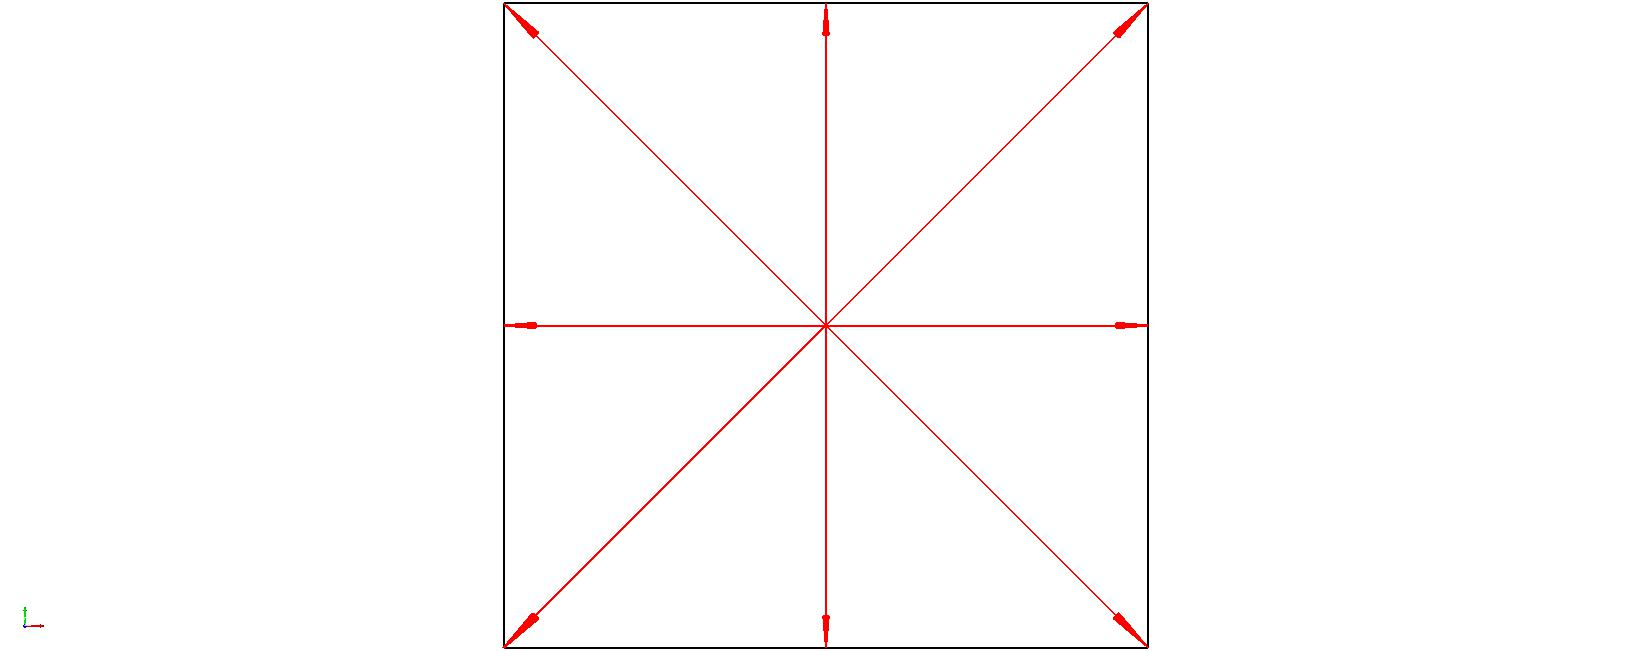
\includegraphics[width=0.95\textwidth]{D2Q9}
        \caption{D2Q9}
    \end{subfigure}
    \begin{subfigure}[t]{0.45\textwidth}
        \centering
        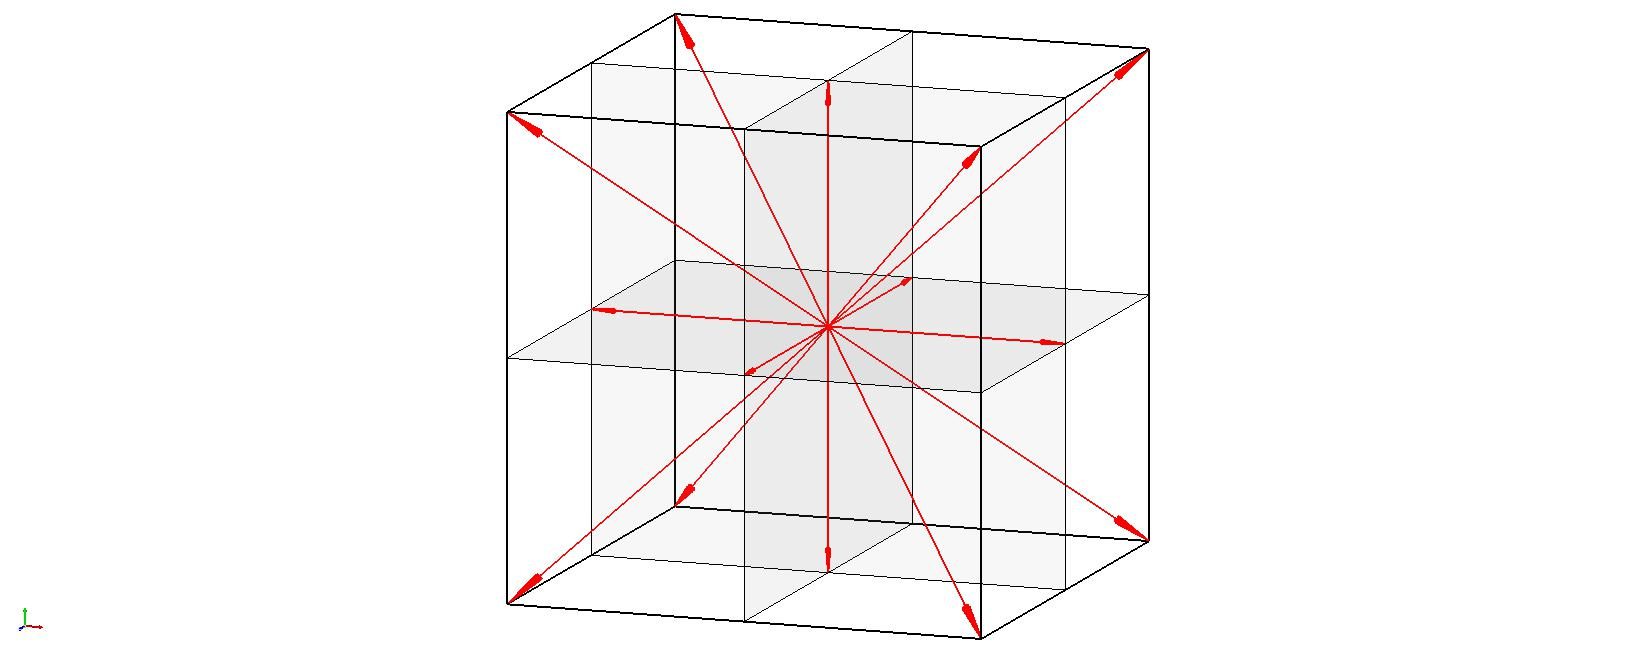
\includegraphics[width=0.95\textwidth]{D3Q15}
        \caption{D3Q15}
    \end{subfigure}    	
	\caption{Velocidades de grilla en los modelos D2Q9 y D3Q15.}
	\label{fig:DdQq}
\end{figure}
\FloatBarrier


\section{Discretizaci\'on del espacio y tiempo}  
Hasta este punto, s\'olo se aplic\'o la discretizaci\'on de la ecuaci\'on de Boltzmann en el espacio de velocidades. El paso final hacia la ecuaci\'on de lattice Boltzmann (en ingl\'es \emph{lattice Boltzman equation} o LBE) debe completarse con la discretizaci\'on del espacio y tiempo.
\nomenclature[A]{LBE}{Ecuaci\'on de lattice Boltzmann (\emph{lattice Boltzmann equation})}
\nomenclature[A]{EDP}{Ecuaci\'on diferencial en derivadas parciales}
\nomenclature[A]{EDO}{Ecuaci\'on diferencial ordinaria}
\par 
La ecuaci\'on de Boltzman discreta (\eq{eq:boltz_disc_vel}) es una ecuaci\'on diferencial en derivadas parciales (EDP) de primer orden y parab\'olica. Una de las t\'ecnicas m\'as usadas en la resoluci\'on de este tipo de ecuaciones es aquella que se conoce como m\'etodo de las caracter\'isticas, que consiste en parametrizar las variables independientes de la EDP para transformarla en una ecuaci\'on diferencial ordinaria (EDO). En este caso, es posible expresar la soluci\'on de \ref{eq:boltz_disc_vel} como $f_{\alpha}=f_{\alpha}(\bm{x}(\zeta),t(\zeta))$, donde $\zeta$ parametriza una trayectoria en el espacio. De esta manera, la \eq{eq:boltz_disc_vel} puede reescribirse usando un diferencial total:
\begin{equation}
	\dfrac{df}{d\zeta} = \dfrac{\partial f}{\partial t}\dfrac{\partial t}{\partial \zeta} + \dfrac{\partial f}{\partial x_{\beta}}\dfrac{\partial x_{\beta}}{\partial \zeta} = \Omega_{\alpha}(\bm{x}(\zeta),t(\zeta))
	\label{eq:zeta_total}
\end{equation}

Por inspecci\'on, debe cumplirse
\begin{equation}
	\dfrac{\partial t}{\partial \zeta} = 1, \qquad
	\dfrac{\partial x_{\beta}}{\partial \zeta} = e_{\alpha\beta}.
\end{equation}
de modo que las soluciones $f_{\alpha}$ siguen una trayectoria dada por $\bm{x}=\bm{x}_0 + \bm{e}_{\alpha}t$, donde $\bm{x}_0$ es una constante arbitraria. Si se considera la trayectoria que pasa a trav\'es del punto $(\bm{x}_0,t_0)$, con $t(\zeta=0)=t_0$ y $\bm{x}(\zeta=0)=\bm{x}_0$, entonces la integraci\'on de la \eq{eq:zeta_total} en un intervalo temporal $\delta_t$ resulta:
\begin{equation}
	f_{\alpha}(\bm{x}_0+\bm{e}_{\alpha}\delta_t,t_0+\delta_t)-f_{\alpha}(\bm{x}_0,t_0)=\int_0^{\delta_t}\Omega_{\alpha}(\bm{x}_0+\bm{e}_{\alpha}\zeta,t_0+\zeta) \, \mbox{d}\zeta.
\end{equation}

Como el punto $(\bm{x}_0,t_0)$ es arbitrario, la integraci\'on puede generalizarse como:
\begin{equation}
	f_{\alpha}(\bm{x}+\bm{e}_{\alpha}\delta_t,t+\delta_t)-f_{\alpha}(\bm{x},t)=\int_0^{\delta_t}\Omega_{\alpha}(\bm{x}+\bm{e}_{\alpha}\zeta,t+\zeta) \, \mbox{d}\zeta.
	\label{eq:elb_integral}
\end{equation}

A partir de la integraci\'on de la \eq{eq:elb_integral} resulta expl\'icito el acople entre la discretizaci\'on espacial y temporal, y se refuerza la practicidad de emplear conjuntos de velocidades que, en un intervalo de tiempo $\delta_t$, se vinculen con las posiciones vecinas en la grilla espacial.
S\'olo resta integral el t\'ermino derecho de la \eq{eq:elb_integral}. Empleando el m\'etodo de Euler expl\'icito, puede obtenerse finalmente la forma popular de la \lbe{}:
\begin{equation}
	f_{\alpha}(\bm{x}+\bm{e}_{\alpha}\delta_t,t+\delta_t)-f_{\alpha}(\bm{x},t)=\delta_t \, \Omega_{\alpha}(\bm{x},t).
	\label{eq:elb}
\end{equation}

La aproximaci\'on de Euler empleada conduce a una representaci\'on de primer orden en la discretizaci\'on de espacio y tiempo. Sin embargo, puede demostrarse que si se realiza dicha integraci\'on mediante el m\'etodo trapezoidal \cite{he_discrete_1998}, y aplicando una redefinici\'on adecuada de la funci\'on de distribuci\'on discreta, es posible obtener una ecuaci\'on igual a (\ref{eq:elb}). Por lo tanto, es posible afirmar que la \eq{eq:elb} constituye una aproximaci\'on de segundo orden tambi\'en en espacio y tiempo.



\section{Operadores de colisi\'on}

Desde un punto de vista cin\'etico, el operador de colisi\'on original de Boltzmann s\'olo es aplicable a simulaciones de gases, ya que \'unicamente considera colisiones binarias entre mol\'eculas. Incluso con estas suposiciones, la descripci\'on formal de este operador es complicada.
\par 
Afortunadamente, el operador de colisi\'on puede simplificarse significativamente en usos pr\'acticos, ya que no es necesario reproducir con exactidud la interacci\'on microsc\'opica de las \fdp{} para determinar el comportamiento macrosc\'opico de un fluido, sino que s\'olo es necesario analizar las cantidades conservadas o momentos. De esta manera, el operador de colisi\'on puede construirse artificialmente, sujeto a las restricciones de conservaci\'on de los momentos adecuados.


\subsection{Operador BGK}

La expresi\'on m\'as sencilla y popular del operador de colisi\'on est\'a basada en la propuesta de Bhatnagar-Gross-Krook (BGK), y considera una relaci\'on lineal entre la funci\'on de distribuci\'on y su versi\'on de equilibrio:
\begin{equation}
	\Omega_{\alpha} = -\dfrac{f_{\alpha} - f_{\alpha}^{eq}}{\tau}.
\end{equation}

Con esta suposici\'on, este operador puede interpretarse como la representaci\'on de la tendencia de $f_{\alpha}$ a alcanzar su estado de equilibrio despu\'es de un tiempo $\tau$. Como se mostr\'o en la \se{sec:cons_macro}, la desviaci\'on de $f$ respecto a su valor de equilibrio est\'a vinculada a propiedades macrosc\'opicas como viscosidad o difusividad t\'ermica y, en consecuencia, al factor de relajaci\'on $\tau$.

Esta aproximaci\'on del operador de colisi\'on funciona en muchos casos, y ha contribuido a expandir la popularidad de la t\'ecnica gracias a la capacidad de reproducir ecuaciones de continuidad con un \'unico factor de relajaci\'on. Sin embargo, esta simplicidad  est\'a asociada a problemas de precisi\'on y estabilidad, que muchas veces s\'olo puede resolverse con incrementos significativos en la resoluci\'on de grilla.


\subsection{Operador MRT}

La aproximaci\'on BGK no es el \'unico mecanismo v\'alido para representar el operador de colisi\'on. Una mejora directa surge de considerar tasas de colisi\'on diferentes para cada componente de la funci\'on de distribuci\'on, $\Omega_{\alpha} = -\Lambda_{\alpha}(f_{\alpha} - f_{\alpha}^{eq})$, lo que da origen a la familia de operadores de colisi\'on de relajaci\'on m\'ultiple \cite{lallemand_theory_2000} (MRT o \emph{multiple relaxation times} por sus siglas en ingl\'es). En este caso, las restricciones de conservaci\'on no se cumplen si los factores de relajaci\'on son diferentes, por lo que es necesario realizar un paso adicional, y considerar la relajaci\'on individual de momentos de la velocidad. De esta manera, la principal diferencia con el operador BGK radica en que la relajaci\'on al estado de equilibrio se realiza en el llamado espacio de momentos, y la resoluci\'on de la \lbe{} se completa volviendo al espacio de poblaciones original.
\nomenclature[A]{MRT}{Tiempo de relajaci\'on m\'ultiple (\emph{multiple relaxation times})}
\nomenclature[A]{SRT}{Tiempo de relajaci\'on simple (\emph{simple relaxation time})}

Los momentos fueron introducidos como sumatorias de la \fdp{} pesada con los polinomios de Hermite. Siguiendo una definici\'on similar, es posible establecer que el momento $m_k$ puede obtenerse en un espacio D$d$Q$q$ a trav\'es de una matriz de transformaci\'on $\bm{M}$ de dimensi\'on $q \times q$:
\begin{equation}
	m_k = \sum_{\alpha=0}^{q-1}M_{k\alpha}f_{\alpha}, \qquad  k=0,\cdots, q-1.
\end{equation}

Esta expresi\'on para los momentos puede reescribirse en notaci\'on vectorial usando:
\begin{equation}
	\begin{gathered}
		\bm{m}=\bm{Mf}, \\
		\bm{m} = (m_0, \cdots, m_{q-1})^T, \\
		\bm{f} = (f_0, \cdots, f_{q-1})^T.
	\end{gathered}
\end{equation}

La idea pricipal detr\'as del operador MRT radica en relajar momentos (en lugar de poblaciones) con tasas individuales. Si la matriz de transformaci\'on $\bm{M}$ se elige adecuadamente, estos los momentos $m_k$ pueden corresponder directamente con los momentos hidrodin\'amicos, como densidad o impulso lineal. Si bien existen numerosas alternativas para construir esta matriz, la m\'as com\'un se basa en definir las filas de $\bm{M}$ usando un conjunto de vectores ortogonales. Como cada fila de $\bm{M}$ produce el mapeo de $f$ a un momento espec\'ifico, es posible tomar los vectores asociados a la densidad y densidad de impulso, y completar el conjunto ortogonal mediante el proceso de Gram-Schmidt. De esta forma, es posible asegurar que los vectores son linealmente independientes y, por lo tanto, $\bm{M}^{-1}$ existe.

La aplicaci\'on del procedimiento de ortogonalizaci\'on genera la siguiente matriz para el espacio D2Q9:
\begin{equation}
	\bm{M}=
	\begin{bmatrix}
	 1 &  1 &  1 &  1 &  1 & 1 &  1 &  1 &  1 \\
	-4 & -1 & -1 & -1 & -1 & 2 &  2 &  2 &  2 \\
	 4 & -2 & -2 & -2 & -2 & 1 &  1 &  1 &  1 \\
	 0 &  1 &  0 & -1 &  0 & 1 & -1 & -1 &  1 \\
	 0 & -2 &  0 &  2 &  0 & 1 & -1 & -1 &  1 \\
	 0 &  0 &  1 &  0 & -1 & 1 &  1 & -1 & -1 \\
	 0 &  0 & -2 &  0 &  2 & 1 &  1 & -1 & -1 \\
	 0 &  1 & -1 &  1 & -1 & 0 &  0 &  0 &  0 \\
	 0 &  0 &  0 &  0 &  0 & 1 & -1 &  1 & -1 \\
	\end{bmatrix}
	\label{eq:MRT_M_D2Q9}
\end{equation} 


mientras que para D3Q15 resulta:
\newpage

\setcounter{MaxMatrixCols}{15}
\begin{equation}
	\bm{M}=
	\begin{bmatrix}
	 1  &  1 &  1 &  1 &  1 & 1 &  1 &  1 &  1 & 1 & 1 & 1 & 1 & 1 & 1 \\
	 -2 & -1 & -1 & -1 & -1 & -1 & -1 & 1 & 1 & 1 & 1 & 1 & 1 & 1 & 1 \\
 	 16 & -4 & -4 & -4 & -4 & -4 & -4 & 1 & 1 & 1 & 1 & 1 & 1 & 1 & 1 \\
 	 0 & 1 & -1 & 0 & 0 & 0 & 0 & 1 & -1 & 1 & -1 & 1 & -1 & -1 & 1 \\
 	 0 & -4 & 4 & 0 & 0 & 0 & 0 & 1 & -1 & 1 & -1 & 1 & -1 & -1 & 1 \\
 	 0 & 0 & 0 & 1 & -1 & 0 & 0 & 1 & -1 & 1 & -1 & -1 & 1 & 1 & -1 \\
 	 0 & 0 & 0 & -4 & 4 & 0 & 0 & 1 & -1 & 1 & -1 & -1 & 1 & 1 & -1 \\
 	 0 & 0 & 0 & 0 & 0 & 1 & -1 & 1 & -1 & -1 & 1 & 1 & -1 & 1 & -1 \\
 	 0 & 0 & 0 & 0 & 0 & -1 & 4 & 1 & -1 & -1 & 1 & 1 & -1 & 1 & -1 \\
 	 0 & 2 & 2 & -1 & -1 & -1 & -1 & 0 & 0 & 0 & 0 & 0 & 0 & 0 & 0 \\
 	 0 & 0 & 0 & 1 & 1 & -1 & -1 & 0 & 0 & 0 & 0 & 0 & 0 & 0 & 0 \\
 	 0 & 0 & 0 & 0 & 0 & 0 & 0 & 1 & 1 & 1 & 1 & -1 & -1 & -1 & -1 \\
 	 0 & 0 & 0 & 0 & 0 & 0 & 0 & 1 & 1 & -1 & -1 & -1 & -1 & 1 & 1 \\
 	 0 & 0 & 0 & 0 & 0 & 0 & 0 & 1 & 1 & -1 & -1 & 1 & 1 & -1 & -1 \\
 	 0 & 0 & 0 & 0 & 0 & 0 & 0 & 1 & -1 & -1 & 1 & -1 & 1 & -1 & 1 \\
	\end{bmatrix}
	\label{eq:MRT_M_D3Q15}
\end{equation} 

Una vez que se conoce la matriz de transformaci\'on $\bm{M}$ s\'olo resta reescribir la \lbe{} para incorporar la relajaci\'on individual de los momentos asociados. La \lbe{} con operador BGK puede escribirse de forma vectorial como:
\begin{equation}
	\bm{f}(\bm{x}+\bm{e}_{\alpha}\delta_t, t+\delta_t) - \bm{f}(\bm{x},t) = -\Lambda \left[ \bm{f}(\bm{x},t) - \bm{f}^{eq}(\bm{x},t) \right],
\end{equation}
donde $\bm{\Lambda} = \Lambda \bm{I}$. En este caso, el operador de colisi\'on permanece inalterado si se introduce una matriz identidad $\bm{I}=\bm{M}^{-1}\bm{M}$:
\begin{equation}
	\begin{aligned}
		\bm{f}(\bm{x}+\bm{e}_{\alpha}\delta_t, t+\delta_t) - \bm{f}(\bm{x},t) &= -\bm{M}^{-1}\bm{M} \Lambda \left[ \bm{f}(\bm{x},t) - \bm{f}^{eq}(\bm{x},t) \right] \\
		&= -\bm{M}^{-1} \Lambda \bm{M} \left[ \bm{f}(\bm{x},t) - \bm{f}^{eq}(\bm{x},t) \right] \\
		&= -\bm{M}^{-1} \Lambda \left[ \bm{M}\bm{f}(\bm{x},t) - \bm{M}\bm{f}^{eq}(\bm{x},t) \right] \\
		&= -\bm{M}^{-1} \Lambda \left[ \bm{m}(\bm{x},t) - \bm{m}^{eq}(\bm{x},t) \right] .	
	\end{aligned}
\end{equation}

Con esta idea, resulta natural extender la definici\'on de $\bm{\Lambda}$ para incorporar la relajaci\'on individual de cada momento usando
\begin{equation}
	\bm{\Lambda}=diag(\Lambda_0, \cdots, \Lambda_{q-1}).
\end{equation}

De esta forma, el uso de un operador de colisi\'on MRT involucra un mapeo del espacio de poblaciones al espacio de momentos usando una matriz de transformaci\'on $\bm{M}$. Si $\bm{M}$ se elige adecuadamente, este proceso permite realizar la relajaci\'on de los momentos hidrodin\'amicos de manera individual, para luego volver a ser transformados al espacio de poblaciones original.




\section{La expansi\'on de Chapman-Enskog}
\label{sec:chapman}

En la \se{sec:ec_boltz} se muestra que existe un v\'inculo directo entre la ecuaci\'on de Boltzmann, los primeros momentos de la \fdp{} y las ecuaciones de conservaci\'on asociadas a la descripci\'on continua de un fluido. Sin embargo, la convergencia hacia una \lbe{} surge como producto de numerosas aproximaciones y simplificaciones, por lo que es necesario evaluar el comportamiento de la forma discreta de la ecuaci\'on de Boltzmann para justificar su uso como t\'ecnica num\'erica de resoluci\'on de mec\'anica de fluidos.

Un m\'etodo robusto para estudiar la relaci\'on entre la \lbe{} discreta y las ecuaciones hidrodin\'amicas recuperadas se conoce con el nombre de an\'alisis de Chapman-Enskog. Esta metodolog\'ia toma su nombre de los matem\'aticos Sydney Chapman y David Enskog, qui\'enes desarrollaron t\'ecnicas para encontrar ecuaciones macrosc\'opicas a partir de la ecuaci\'on de Boltzmann con el operador de colisi\'on original \cite{chapman_mathematical_1970}. Esencialmente, este an\'alisis consiste en una expansi\'on o perturbaci\'on de $f_{\alpha}$ en torno a la distribuci\'on de equilibrio $f_{\alpha}^{eq}$, utilizando el n\'umero de Knudsen (Kn) como par\'ametro de expansi\'on. Como se detalla en la \se{sec:cons_macro}, si $f \simeq f^{eq}$ entonces es posible recuperar las ecuaciones de Euler. Por lo tanto, cualquier comportamiento diferente al de estas ecuaciones est\'a vinculado a los t\'erminos de no-equilibrio, es decir, a aquellas desviaciones de la distribuci\'on de equilibrio que se explicitan con la expansi\'on de Chapman-Enskog.
\nomenclature[N]{Kn}{N\'umero de Knudsen}

T\'ipicamente, la expansi\'on de $f_{\alpha}$ se realiza usando el par\'ametro $\varepsilon^n$ para indicar los t\'erminos de orden Kn$^n$. De esta manera, los componentes de la \fdp{} discreta se escriben como:
\begin{equation}
	f_{\alpha} = \sum_{n} \varepsilon^{n} f_{\alpha}^{(n)},
	\label{eq:f_che_gral}
\end{equation}
donde $f_{\alpha}^{(0)} = f_{\alpha}^{eq}$. Como destaca Kr\"uger \cite{kruger_lattice_2017}, un concepto central de esta perturbaci\'on implica que, en una ecuaci\'on perturbada, cada orden en Kn forma una ecuaci\'on semi-independiente. De esta manera, cada ecuaci\'on posee un v\'inculo con el orden siguiente y este v\'inculo s\'olo incorpora t\'erminos de correcci\'on, por lo que simplemente es necesario evaluar una cantidad reducida de \'ordenes. 

El camino cl\'asico usado para completar el an\'alisis de expansi\'on consiste en expresar las componentes de una \lbe{} como funciones definidas en $(\bm{x},t)$, y aplicar la expansi\'on a las \fdp{} y a los operadores diferenciales. Si se preservan los t\'erminos correspondientes a los primeros \'ordenes de $\varepsilon$, es posible separar la ecuaci\'on expandida en un conjunto de ecuaciones correspondientes a cada escala. De esta manera, tomando momentos a cada ecuaci\'on y luego recombinando, es posible encontrar cu\'ales son las ecuaciones macrosc\'opicas recuperadas. En particular, esta metodolog\'ia permite demostrar que si se implementa la \lbe{} de la \eq{eq:elb}, con operador de colisi\'on BGK y distribuci\'on de equilibrio dada por la \eq{eq:feq}, entonces las variables macrosc\'opicas $\rho$ y $\bm{u}$ satisfacen:
\begin{subequations}
	\begin{equation}
		\dfrac{\partial \rho}{\partial t}  + \nabla \cdot (\rho \bm{u})=0
	\end{equation}
	\begin{equation}
	\dfrac{\partial (\rho \bm{u})}{\partial t}  + \nabla \cdot (\rho \bm{u}\bm{u})=-\nabla \cdot (\rho c_s^2 \bm{I}) + \nabla \cdot [\rho \nu (\nabla \bm{u}+\nabla \bm{u}^T)]
	\end{equation}
\end{subequations}

Este conjunto de ecuaciones, similar a Navier-Stokes, contiene un t\'ermino de presi\'on asociado a una ecuaci\'on de estado (\emph{equation of state} o EOS por sus siglas en ng\'es), y presenta una viscosidad cinem\'atica que est\'a relacionada con el factor de relajaci\'on:
\begin{equation}
	\nu = c_s^2 \left( \tau - \dfrac{\delta_t}{2} \right).
\end{equation}

La aplicaci\'on de este an\'alisis y la evaluaci\'on de sus resultados no es directa ni trivial. Sin embargo, en la bibliograf\'ia existen numerosos ejemplos del uso de esta t\'ecnica en el an\'alisis de las formas m\'as sencillas de ecuaciones de Boltzmann discretas \cite{kruger_lattice_2017, succi_lattice_2001, succi_lattice_2018, guo_lattice_2013}. Por otro lado, en los Cap\'itulos \ref{chap:modelo2D} y \ref{chap:modelo3D} se muestra, de manera detallada, c\'omo es el procedimiento necesario para efectuar el an\'alisis de Chapman-Enskog sobre ecuaciones con operador de colisi\'on MRT y t\'erminos de fuente.

% por lo que resulta conveniente ejemplificar su uso mediante el an\'lisis de una de las expresiones m\'as sencillas de lattice Boltzmann:, una \lbe{} con operador BKG, sin t\'erminos de fuerza y con una distribuci\'on de equilibrio dada por la \eq{eq:feq}. En este caso, el m\'etodo se resume como:
%\begin{subequations}
%	\begin{equation}
%		f_{\alpha}(\bm{x}+\bm{e}_{\alpha}\delta_t,t+\delta_t)-f_{\alpha}(\bm{x},t)= -\dfrac{1}{\tau} \left[ f_{\alpha}(\bm{x},t) - f^{eq}_{\alpha}(\bm{x},t) \right] \delta_t
%		\label{eq:chex_lbe}
%	\end{equation}
%	\begin{equation}
%		f_{\alpha}^{eq} = w_{\alpha} \rho \left[ 1 + \dfrac{e_{\alpha \beta}u_{\beta}}{c_s^2} + \dfrac{u_{\beta}u_{\gamma}(e_{\alpha \beta}e_{{\alpha}\beta}-c_s^2\delta_{\beta\gamma})}{2c_s^4} \right]
%	\end{equation}
%	\begin{equation}
%		\rho = \sum_{\alpha} f_{\alpha}
%	\end{equation}
%	\begin{equation}
%		\rho = \sum_{\alpha} \bm{e}_{\alpha} f_{\alpha}
%	\end{equation}
%\end{subequations}
%
%El primer paso del an\'alisis de Chapman-Enskog consiste en expresar todos los t\'erminos de la \lbe{} en funciones definidas en $(\bm{x},t)$. En particular, mediante un desarrollo en serie de Taylor de dos variables es posible escribir \cite{qian_lattice_1992}:
%\begin{equation}
%	f_{\alpha} (\bm{x} + \bm{e}_{\alpha}\delta_t, t+\delta_t) = \sum_{k=0}^{\infty}  \dfrac{1}{k!} D_{\alpha}^{(k)} f_{\alpha} (\bm{x},t) \delta_t^{2},
%\end{equation}
%donde $D_{\alpha}^{(k)}=(\partial_t + \bm{e}_{\alpha} \cdot \nabla)^k$. Eliminando la dependencia $(\bm{x},t)$ por claridad, la \eq{eq:chex_lbe} puede reescribirse conservando los t\'erminos de orden $O(\delta_t^2)$:
%\begin{equation}
%	\delta_t D_{\alpha}f_{\alpha} + \dfrac{\delta_t^2}{2}D_{\alpha}^2 f_{\alpha} = -\dfrac{1}{\tau} (f_{\alpha} - f_{\alpha}^{eq}).
%	\label{eq:f_taylor_gral}
%\end{equation}
%
%Por otro lado, el an\'alisis multiescala no s\'olo implica expandir $f_{\alpha}$ en potencias de $\varepsilon$, sino que adem\'as es necesario expandir las escalar temporales y espaciales. En este caso es suficiente considerar $t = \varepsilon t_1 + \varepsilon^2 t_2$ y $x_{\beta}=\varepsilon x_{\beta_1}$, de modo que las derivadas parciales correspondientes resultan:
%
%\begin{subequations}
%
%	\begin{equation}
%		\dfrac{\partial}{\partial t} = \varepsilon \dfrac{\partial}{\partial t_1} + 	\varepsilon^2 \dfrac{\partial}{\partial t_2}
%	\end{equation}
%	\begin{equation}
%		\dfrac{\partial}{\partial x_{\beta}} = \varepsilon \dfrac{\partial}{\partial x_{\beta_1}}
%	\end{equation}
%	\label{eq:escalas_che_gral}
%\end{subequations}
%
%Si se reemplazan las expansiones dadas por las \eqs{eq:f_che_gral}{eq:escalas_che_gral} en la \eq{eq:f_taylor_gral}, y se conservan \'unicamente los t\'erminos de expansi\'on hasta orden $\varepsilon^2$, se obtiene:
%\begin{equation}
%	\varepsilon D_{\alpha}^{(1)} f_{\alpha}^{(0)} +
%    \varepsilon^2 D_{\alpha}^{(1)} f_{\alpha}^{(1)} + 
%    \varepsilon^2 \dfrac{\partial}{\partial t_1} f_{\alpha}^{(0)} 
%    + \dfrac{\delta_t}{2} \varepsilon^2 D_{\alpha}^{(1)^2} f_{\alpha}^{(0)} = 	-\dfrac{1}{\tau \delta_t}( f_{\alpha}^{(0)} + \varepsilon f_{\alpha}^{(1)} + \varepsilon^2 f_{\alpha}^{(2)} - f_{\alpha}^{eq}).
%\end{equation}
%
%En esta ecuaci\'on, el operador $D^{(1)}$ contiene las derivadas en las primeras escalas, es decir $D_{\alpha}^{(1)} = \partial_{t_1} + \bm{e}_{\alpha} \cdot \nabla_1$. Como se mencion\'o previamente, uno de los conceptos principales de este tipo de an\'alisis implica que cada escala de expansi\'on puede evaluarse mediante una ecuaci\'on semi-independiente. Por lo tanto, si se separa en potencias de $\varepsilon$ es posible generar un conjunto de ecuaciones paa cada escala:
%
%\begin{subequations}
%	\begin{align}
%		\varepsilon^0: && f_{\alpha}^{(0)} = f_{\alpha}^{eq} \label{eq:eps_0_gral}\\
%		\varepsilon^1: &&  D_{\alpha}^{(1)} f_{\alpha}^{(0)} = -\dfrac{1}{\tau \delta_t} f_{\alpha}^{(1)} \label{eq:eps_1_gral}\\
%		\varepsilon^2: && \left( 1 - \dfrac{1}{2 \tau} \right) D_{\alpha}^{(1)} f_{\alpha}^{(1)} + \dfrac{\partial}{\partial t_2} f_{\alpha}^{(2)} =  -\dfrac{1}{\tau \delta_t} f_{\alpha}^{(2)} \label{eq:eps_2_gral}
%	\end{align}
%\end{subequations}



\section{Lattice Boltzmann como m\'etodo num\'erico}

La representaci\'on discreta de la ecuaci\'on de Boltzmann y sus principales momentos, junto con la construcci\'on adecuada de un operador de colisi\'on artificial, constituyen una t\'ecnica que permite, en principio, simular el comportamiento de fluidos. Por otro lado, la incorporaci\'on del an\'alisis de Chapman-Enskog permite verificar formalmente cu\'al es el comportamiento hidrodin\'amico macrosc\'opico, de modo que se logra alcanzar un conjunto de caracter\'isticas que permiten clasificar a LB como un m\'etodo num\'erico para mec\'anica de fluidos.

A diferencia de las t\'ecnicas tradicionales, con LB no se resuelven directamente las ecuaciones diferenciales de inter\'es, sino que su soluci\'on se obtiene de manera indirecta, es decir, a partir de la soluci\'on de otro tipo de ecuaciones. En este caso, se realiza el transporte de una \fdp{} en una grilla regular, con momentos discretos que est\'an asociados a propiedades macrosc\'opicas del fluido. Si bien existen numerosas variantes del m\'etodo, desarrolladas para incorporar caracter\'isticas particulares de cada tipo de flujo, o aspectos num\'ericos como precisi\'on y estabilidad, la integraci\'on de la ecuaci\'on de Boltzmann mediante el m\'etodo de caracter\'isticas da origen al algoritmo t\'ipico de LB, como se ejemplifica con el operador BGK:
\begin{equation}
	\underbrace{ \phantom{\dfrac{1}{\tau}} f_{\alpha}(\bm{x}+\bm{e}_{\alpha}\delta_t, t+\delta_t)}_{\mbox{advecci\'on}} = 
	\underbrace{ f_{\alpha}(\bm{x},t) -\dfrac{1}{\tau} \left[ f_{\alpha}(\bm{x},t) - f_{\alpha}^{eq}(\bm{x},t) \right]\delta_t}_{\mbox{colisio\'n}}
\end{equation}

Como se muestra en la ecuaci\'on, la implementaci\'on num\'erica de una \lbe{} contiene dos partes claramente identificables. Por un lado, la relajaci\'on de cada componente (o de los diferentes momentos en un operador MRT), tiene lugar durante el proceso conocido como colisi\'on. Durante esta etapa, t\'ipicamente se realizan operaciones locales sobre la \fdp{}, es decir, empleando informaci\'on de variables definidas en $(\bm{x},t)$. Despu\'es de esta instancia, las componentes de la \fdp{} se asocian a un estado conocido como post-colisi\'on, usualmente denotado como $f_{\alpha}^*$. 

La segunda etapa del algoritmo LB general, conocida como advecci\'on o \emph{streaming}, consiste en el desplazamiento de las componentes de post-colisi\'on hacia los nodos vecinos. Como se muestra esquem\'aticamente en la \fig{fig:lb_str_col}, cada componente $f_{\alpha}^*$ debe reposicionarse en el nodo vecino conectado por la velocidad de grilla corespondiente.

\begin{figure}[htb]
    \centering
    \begin{subfigure}[t]{0.45\textwidth}
        \centering
        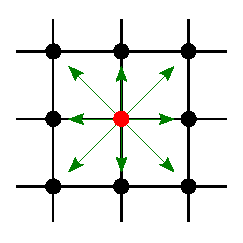
\includegraphics[width=0.95\textwidth]{colision}
        \caption{Colisi\'on}        
    \end{subfigure}
    \begin{subfigure}[t]{0.45\textwidth}
        \centering
        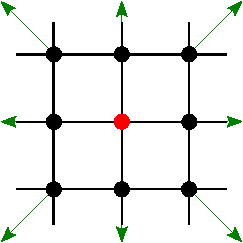
\includegraphics[width=0.95\textwidth]{streaming}
        \caption{Advecci\'on}        
    \end{subfigure}
    \caption{Representaci\'on esquem\'atica de las etapas principales de la soluci\'on de una \lbe{}.}
    \label{fig:lb_str_col}
\end{figure}
%\FloatBarrier

Durante el desarrollo de la etapa de colisi\'on es necesario involucrar a las variables macrosc\'opicas definidas a tiempo $t$, a trav\'es de la funci\'on de distribuci\'on o t\'erminos de fuente adicionales. Como esta informaci\'on es requerida numerosas veces durante un mismo paso de tiempo, es conveniente definir (computacionalmente) expl\'icitamente a las variables macrosc\'opicas y actualizar los valores de cada nodo s\'olo una vez por paso de tiempo. Con esta alternativa se construye el algoritmo general para la resoluci\'on de una \lbe{}, con los pasos que se resumen en el esquema de la \fig{fig:lb_algo}. Este mecanismo de resoluci\'on es el empleado en el desarrollo de esta tesis.
\begin{figure}[ht]
	\centering
	\begin{tikzpicture}[node distance = 2.5cm, auto]
    		% nodes
		\node [block] (init) {Inicializaci\'on \\ $\rho_i$, $\bm{u}_i$, \\ $f=f^{eq}(\rho_i,\bm{u}_i)$};
	    \node [block, below of=init] (col) {Colisi\'on \\ $f^* = \Omega(f)$};
	    \node [block, below of=col] (adv) {Advecci\'on};
	    \node [block, below of=adv] (cdb) {Condiciones de contorno};
	    \node [block, below of=cdb] (macro) {Actualizaci\'on \\ $\rho$, $\bm{u}$};
	    \node [decision, below of=macro] (decide) {?`Tiempo final?};
    	    \node [block, below of=decide, node distance=3cm] (fin) {Fin};
	    
	    % Edges
	    \path [line] (init) -- (col);
	    \path [line] (col) -- (adv);
	    \path [line] (adv) -- (cdb);
	    \path [line] (cdb) -- (macro);
	    \path [line] (macro) -- (decide);
	    \path [line] (decide) -- node {s\'i} (fin);
	    \path [line] (decide) -- +(-3,0) |- node [near start, sloped, above] {no. $t + \delta_t$} (col);	
	\end{tikzpicture}	
	\caption{Algoritmo LB general}
	\label{fig:lb_algo}
\end{figure}
\FloatBarrier



En la \fig{fig:lb_algo} se muestra un paso adicional (y fundamental) del algoritmo, que consiste en la implementaci\'on de condiciones de contorno. Despu\'es del paso de advecci\'on, los nodos ubicados sobre la frontera del dominio computacional contienen componentes que no pueden ser actualizadas, ya que no existen nodos vecinos en ciertas direcciones. En el caso de LB, esta informaci\'on puede reconstruirse con m\'etodos espec\'ificos para obtener el comportamiento hidrodin\'amico deseado, como restricciones en el valor de las variables macrosc\'opicas sobre paredes, condiciones peri\'odicas o de flujo saliente. En los cap\'itulos siguientes se aborda en detalle la incorporaci\'on de \'estos m\'etodos al algoritmo.

En su conjunto, LB es un m\'etodo que permite obtener la soluci\'on de ecuaciones de conservaci\'on sin necesidad de abordarlas directamente. La integraci\'on de la ecuaci\'on de Boltzmann mediante el m\'etodo de las caracter\'isticas conduce a una \lbe{} expl\'icita, y que presenta una convergencia de segundo orden en las coordenadas espaciales y temporal. Este resultado impacta significativamente en la eficiencia computacional del m\'etodo, ya que no es necesario resolver costosos sistemas de ecuaciones, como el correspondiente a la ecuaci\'on de Poisson para la presi\'on en los m\'etodos tradicionales. Por otro lado, el paso de advecci\'on simplifica el tratamiento de los t\'erminos convectivos no lineales de la ecuaci\'on de conservaci\'on de impulso. De esta manera se obtiene una t\'ecnica cuyo costo computacional global depende linealmente del n\'umero de nodos de la grilla, y con un algoritmo que facilita su implementaci\'on en sistemas de procesamiento distribuido. 

Sin embargo, esta aparente simplicidad tiene su precio. La mayor\'ia de los modelos LB presentan restricciones significativas de estabilidad, lo que limita su utilizaci\'on en la simulaci\'on de flujos con, por ejemplo, baja viscosidad. Si bien los operadores de colisi\'on MRT presentan rangos de estabilidad sensiblemente superiores a los BGK, a\'un sigue siendo insuficiente para determinadas aplicaciones. Por otro lado, el v\'inculo entre la \lbe{} y las ecuaciones macrosc\'opicas no siempre es sencillo de cuantificar. La expansi\'on de Chapman-Enskog est\'a basada en un an\'alisis asint\'otico, de modo que los resultados de las simulaciones pueden mostrar efectos de los t\'erminos de orden superior no considerados. Estas caracter\'isticas negativas deben ser consideradas al momento de aplicar la t\'ecnica, pero si su uso es factible, las limitaciones son ampliamente compensadas por la eficiencia y simplicidad del m\'etodo.


\section{Conclusiones}

El m\'etodo de lattice Boltzmann ha evolucionado hasta convertirse en una herramienta robusta y fiable para la simulaci\'on num\'erica de mec\'anica de fluidos. Desde un punto de vista formal, LB puede entenderse como un camino para resolver una ecuaci\'on de Boltzmann: en lugar de discretizar directamente aquellas ecuaciones de inter\'es, el m\'etodo propone transportar una funci\'on de distribuci\'on en una grilla regular, considerando que los momentos (en el espacio de fases) de esta \fdp{} est\'an asociados a las principales magnitudes hidrodin\'amicas de las ecuaciones macrosc\'opicas de inter\'es, como densidad, velocidad o temperatura. A trav\'es de t\'ecnicas de expansi\'on multiescala, como el an\'alisis de Chapman-Enskog, es posible verificar que una adecuada elecci\'on de grilla espacial, velocidades discretas del espacio de fases, y operador de colisi\'on, pueden ser combinadas adecuadamente para obtener la soluci\'on de ecuaciones de conservaci\'on de t\'ipicas de mec\'anica de fluidos. 

\chapter{Simulaci\'on de flujo multif\'asico}

\section{Lattice Boltzmann para flujo multif\'asico}
En sinton\'ia con el crecimiento de la mec\'anica de fluidos computacional, fueron desarroll\'andose numerosos m\'etodos num\'ericos macrosc\'opicos destinados a resolver las ecuaciones de Navier-Stokes en flujos multif\'asicos \cite{scardovelli_direct_1999}. Entre los m\'etodos m\'as populares, pueden destacarse el de \textbf{front-tracking}, el m\'etodo Volume of Fluid (VOF) y el m\'etodo level set. A pesar de la amplia difusi\'on adquirida, y de la demostrada capacidad para resolver con precisi\'on diversos escenarios con flujos multif\'asicos, estas t\'ecnicas tradicionales contin\'uan presentando limitaciones que dificultan el modelado de problemas complejos con transferencia de calor, como ebullici\'on y condensaci\'on. En particular, el m\'etodo de \textbf{front-tracking} generalmente no permite simular adecuadamente procesos de coalescencia y ruptura de una interfase \cite{scardovelli_direct_1999,liu_three-dimensional_2012}. La aplicaci\'on de VOF y level set suele requerir pasos de reconstrucci\'on o reinicializaci\'on de la interfase, que pueden no ser f\'isicos y complejos de implementar \cite{liu_three-dimensional_2012}. Adem\'as, suelen originarse inestabilidades num\'ericas en el uso de VOF o level set para simular flujos dominados por tensi\'on superficial en geometr\'ias complejas \cite{scardovelli_direct_1999}.
\par
En comparaci\'on con otros m\'etodos computacionales, el MLB presenta ventajas adicionales para la simulaci\'on de flujos complejos. Por un lado, la naturaleza mesosc\'opica con base en la teor\'ia cin\'etica molecular permite generar modelos con s\'olidos fundamentos termodin\'amicos. Por otro lado, es posible incorporar directamente el uso de ecuaciones de estado en la resoluci\'on de Navier-Stokes en escala macrosc\'opica, lo que a su vez elimina la necesidad de resolver una ecuaci\'on de Poisson para la presi\'on. Finalmente, la mayor\'ia de los modelos son sencillos de programar, y la naturaleza local de las operaciones involucradas facilita la explotaci\'on de arquitecturas con paralelismo masivo, como las unidades de procesamiento gr\'afico (GPU).
\par 
Las mencionadas caracter\'isticas han motivado el desarrollo de esquemas para flujo multif\'asico desde los or\'igenes del m\'etodo. A pesar de que se ha conformado un enorme universo de modelos diferentes, la gran mayor\'ia de estas alternativas pueden agruparse dentro de cuatro categor\'ias principales: color-gradient \cite{liu_three-dimensional_2012,gunstensen_lattice_1991}, pseudopotential \cite{shan_lattice_1993,shan_simulation_1994,chen_critical_2014}, free-energy \cite{swift_lattice_1996,inamuro_galilean_2000} y phase-field \cite{he_lattice_1999,liang_phase-field-based_2014}. 

\subsection*{Color-gradient}
El m\'etodo color-gradient fue introducido por Gunstensen et al. \cite{gunstensen_lattice_1991}, como una versi\'on mejorada del modelo LGA multif\'asico de Rothman y Keller \cite{rothman_immiscible_1988}. En este modelo las fases se denotan con diferentes colores, y la interacci\'on entre part\'iculas, responsable de la separaci\'on de fases, es modelada con gradientes locales de color asociado a la diferencia de densidad entre ambas fases. Tomando como ejemplo un sistema de dos fases, el modelo color-gradient original usa dos tipos de funciones de distribuci\'on, $f_{ri}$ y $f_{bi}$, para representar a los fluidos rojo y azul respectivamente. La distribuci\'on total de la mezcla $f_i = f_{ri}+f_{bi}$ evoluciona como:
\begin{equation}
	f_i(\bm{x}+\bm{e}_i\delta_t,t+\delta_t) - f_i(\bm{x},t) = \Omega_i^c + \Omega_i^p,
\end{equation}
donde $\Omega_i^c$ denota los efectos de colisi\'on y $\Omega_i^p$ se encuentra relacionado con la tensi\'on interfacial. En este caso, las densidades y velocidades para cada fase se definen como
\begin{equation}
	\begin{gathered}
	\rho_k = \sum_i f_{ki}, \qquad \rho_k\bm{u}_k = \sum_i \bm{e}_if_{ki}, \qquad k=r,b, \\
	\rho = \rho_r + \rho_b, \qquad \rho\bm{u} = \rho_r\bm{u}_r + \rho_b\bm{u}_b.
	\end{gathered}
\end{equation}

Si bien es posible emplear un operador LBGK para $\Omega_i^c$, el t\'ermino $\Omega_i^p$ se calcula empleando un par\'ametro de orden que tiene en cuenta la diferencia de densidad entre fases. Despu\'es de la colisi\'on, las funciones de distribuci\'on parciales son sometidas a un paso de ajuste de color antes del streaming. Estos pasos adicionales del algoritmo contribuyen a producir inestabilidades num\'ericas, a la vez que reducen de forma dr\'astica la eficiencia computacional por paso de tiempo \cite{guo_lattice_2013}.

\subsection*{Free-energy}
El m\'etodo free-energy fue propuesto originalmente por Swift et al. \cite{swift_lattice_1996}, y presenta un punto de partida asociado a consideraciones termodin\'amicas b\'asicas. La idea detr\'as de estos m\'etodos consiste en derivar una funci\'on de distribuci\'on de equilibrio adecuada, de forma que el momento de segundo orden correspondiente incluya un tensor de presi\'on termodin\'amico no ideal. En particular, este tensor se deriva a partir de la energ\'ia libre de un fluido asociado a una ecuaci\'on de estado de Van der Waals, y puede escribirse como:
\begin{equation}
	P^{'}_{\alpha\beta}=p\delta_{\alpha\beta}+\kappa\dfrac{\partial \rho}{\partial x_{\alpha}}\dfrac{\partial \rho}{\partial x_{\beta}}
\end{equation}
donde $\kappa$ es una constante asociada al valor de tensi\'on superficial en la interfase. Para lograr la recuperaci\'on de este tensor, Swift et al. sugirieron el uso de una ELB con operador de colisi\'on LBGK
\begin{equation}
	f_i(\bm{x}+\bm{e}_i\delta_t,t+\delta_t) - f_i(\bm{x},t) = -\dfrac{1}{\tau}\left[ f_i - f_i^{eq}(\rho, \bm{u}, \nabla\bm{u}) \right],
\end{equation}
mientras que la distribuci\'on de equilibrio satisface las siguientes restricciones:
\begin{equation}
	\sum_i f_i^{eq} = \rho, \qquad \sum_i \bm{e}_if_{i}=\rho\bm{u}, \qquad
	\sum_i \bm{e}_i\bm{e}_if_{i}= \bm{P}^{'}+\rho\bm{u}\bm{u}
	\label{eq:free_energy+rest}
\end{equation}

De forma similar a lo que ocurre con el modelo est\'andar para flujos de una \'unica fase, $f^{eq}$ puede escribirse como un polinomio de $\bm{u}$:
\begin{subequations}
	\begin{equation}
		f_i^{eq}=A + B(\bm{e}_i \cdot \bm{u}) + C u^2 + D(\bm{e}_i \cdot \bm{u})^2 + G:\bm{e}_i\bm{e}_i, \qquad i\neq 0,
	\end{equation}
	\begin{equation}
		f_i^{eq}=A_0 + C_0 u^2, \qquad i = 0.
	\end{equation}
\end{subequations}

Los coeficientes de $f_i^eq$ para una grilla bidimensional pueden obtenerse empleando las restricciones de la \eq{eq:free_energy+rest}:
\begin{equation}
	\begin{gathered}
		A_0 = \rho - 6 A, \qquad C_0 = -\rho, \\
		A = \dfrac{1}{3}(p_0-\kappa \rho \nabla^2 \rho), \qquad B = \dfrac{\rho}{3}, \qquad C = -\dfrac{\rho}{6}, \qquad  D = \dfrac{2\rho}{3},  \\
		G_{xx} = -G_{yy} = \dfrac{\kappa}{3}\left[ \left(\dfrac{\partial \rho}{\partial x}\right)^2 - \left(\dfrac{\partial \rho}{\partial y}\right)^2 \right], \qquad G_{xy}=\dfrac{2\kappa}{3}\dfrac{\partial \rho}{\partial x} \dfrac{\partial \rho}{\partial y}.
	\end{gathered}
\end{equation}

De esta forma, las ecuaciones macrosc\'opicas recuperadas usando el m\'etodo de Swift resultan:
\begin{equation}
	\dfrac{\partial \rho}{\partial t} + \nabla \cdot (\rho \bm{u}) = 0,
\end{equation}
\begin{align}
	\dfrac{\partial \rho \bm{u}}{\partial t} + \nabla \cdot (\rho \bm{uu}) =& -\nabla p_0 + \nu \nabla^2 (\rho \bm{u})+\nabla[\lambda \nabla \cdot (\rho \bm{u})]		\\
	&-\left( \tau - \dfrac{1}{2} \right)\dfrac{\partial p_0}{\partial \rho} \delta_t \nabla \cdot [\bm{u}\nabla \rho + (\nabla \rho)\bm{u}],
\end{align}
donde 
\begin{equation}
	\nu = \dfrac{\delta_t}{4}\left( \tau - \dfrac{1}{2} \right), \qquad \lambda = \delta_t\left( \tau - \dfrac{1}{2} \right)\left( \dfrac{1}{2} - \dfrac{\partial p_0}{\partial \rho}\right)
\end{equation}

\textcolor{red}{Falta decir q\'ue es $p_0$.}

Las primeras versiones asociadas a esta familia sufrieron la falta de invariancia galileana debido a la recuperaci\'on de t\'erminos que no est\'an relacionados con Navier-Stokes, originados por la misma incorporaci\'on del tensor de presi\'on en la distribuci\'on de equilibrio \cite{kuzmin_multi-relaxation_2008}. Para recuperar esta invarianza es necesario, por lo tanto, incorporar t\'erminos de correcci\'on en la funci\'on de distribuci\'on de equilibrio. Este tipo de adaptaciones son similares a aquellas adoptadas por las versiones posteriores de los m\'etodos dentro de la familia color-gradient, y usualmente constituyen fuentes adicionales de inestabilidad num\'erica al incorporar t\'erminos como $\bm{u}\nabla\rho$ y $\bm{u}\cdot\nabla\rho$.

\subsection*{Phase-field}
Esta categor\'ia representa a los modelos basados en la teor\'ia de phase-field, es decir, aquellos en los que la din\'amica de la interfase se encuentra descripta por un par\'ametro de orden regido por una ecuaci\'on de Cahn-Hilliard o similar \cite{jacqmin_calculation_1999}. Esta aproximaci\'on a la simulaci\'on de flujos multif\'asicos con LB tiene su contraparte equivalente dentro de las t\'ecnicas tradicionales de CFD para modelos de interfase difusa, como el de Ding et. al \cite{ding_diffuse_2007}.

La versi\'on original de He at al. \cite{he_lattice_1999} hace uso de dos funciones de distribuci\'on, $g$ y $f$, para recuperar las ecuaciones de Navier-Stokes y una del tipo Cahn-Hilliard para la evoluci\'on de la interfase respectivamente. Usando operadores de colisi\'on LBGK, las ecuaciones corresponden a:
\begin{equation}
	g_i(\bm{x}+\bm{e}_i\delta_t,t+\delta_t) - g_i(\bm{x},t) = -\dfrac{1}{\tau_1}\left[ g_i(\bm{x},t) - g_i^{eq}(\bm{x},t) \right] + S_i(\bm{x},t)\delta_t,
	\label{eq:he_g_eq}
\end{equation}
\begin{equation}
	f_i(\bm{x}+\bm{e}_i\delta_t,t+\delta_t) - f_i(\bm{x},t) = -\dfrac{1}{\tau_2}\left[ f_i(\bm{x},t) - f_i^{eq}(\bm{x},t) \right] + S_i^{'}(\bm{x},t)\delta_t,
\end{equation}
donde la viscosidad cinem\'atica se recupera mediante $\nu=(c_s^2)(\tau_1-0.5)\delta_t$, $\tau_2$ se relaciona con la mobilidad de la ecuaci\'on de Cahn-Hilliard, y $S_i$, $S_i^{'}$ son t\'erminos de fuente. Las funciones de distribuci\'on de equilibrio se definen mediante:
\begin{equation}
	g_i^{eq} = w_i\left[ p + \rho c_s^2 \left( \dfrac{e_{i\alpha}u_{\alpha}}{c_s^2}  + \dfrac{e_{i\alpha}u_{\alpha}e_{i\beta}u_{\beta}}{2c_s^4} - \dfrac{u_{\alpha}u_{\alpha}}{2c_s^2} \right)  \right]
\end{equation}
\begin{equation}
	f_i^{eq} = w_i \phi \left[ 1 +  \dfrac{e_{i\alpha}u_{\alpha}}{c_s^2}  + \dfrac{e_{i\alpha}u_{\alpha}e_{i\beta}u_{\beta}}{2c_s^4} - \dfrac{u_{\alpha}u_{\alpha}}{2c_s^2}  \right]
\end{equation}
donde $p$ corresponde a la presi\'on hidrodin\'amica. $\phi$ es el par\'ametro de orden que se utiliza, por ejemplo, para determinar la distribuci\'on de densidad:
\begin{equation}
	\rho(\phi) = \rho_g + \dfrac{\phi - \phi_g}{\phi_l - \phi_g}(\rho_l - \rho_g)
\end{equation}

En este caso, los sub\'indices $l$ y $g$ corresponden a las fases l\'iquida y gaseosa respectivamente. Las variables macrosc\'opicas del modelo de He et al. se calculan como:
\begin{equation}
	\begin{gathered}
		\phi = \sum_i f_i \\
		p = \sum_i g_i - \dfrac{\delta_t}{2} u_{\beta} \dfrac{\partial(p - \rho c_s^2)}{\partial x_{\beta}} \\
		\rho u_{\alpha}c_s^2 = \sum_i e_{i\alpha}g_i + \dfrac{\delta_t}{2}c_s^2 F_{\alpha}
	\end{gathered}
	\label{eq:he_macro_variables}
\end{equation}
donde $F_{\alpha}$ representa las fuerzas externas, incluyendo las asociadas a la tensi\'on interfacial. La expansi\'on de Chapman-Enskog de las Ecs.~\eqref{eq:he_g_eq}-\eqref{eq:he_macro_variables} muestra que las ecuaciones macrosc\'opicas recuperadas resultan:
\begin{equation}
	\begin{gathered}
		\dfrac{\partial (\rho \bm{u})}{\partial t} + \nabla \cdot (\rho \bm{uu})  = -\nabla p  + \nu \nabla \cdot \left[ \rho (\nabla\bm{u} + \nabla \bm{u}^T) \right] + \bm{F} \\
		\dfrac{\partial \phi}{\partial t} + \nabla \cdot (\phi \bm{}u) = \dfrac{1}{2} \left( 1 - \dfrac{1}{2\tau_2} \right) \nabla^2 (p - c_s^2 \phi)
	\end{gathered}
\end{equation}

\subsection*{Pseudopotential}
El m\'etodo pseudopotencial, que podr\'ia considerarse como la t\'ecnica m\'as sencilla para simular flujos multif\'asicos, fue propuesta por Shan y Chen \cite{shan_lattice_1993,shan_simulation_1994}. En este m\'etodo, las interacciones entre part\'iculas fluidas son imitadas mediante un potencial interpart\'icula, de modo que la separaci\'on de fases ocurre autom\'aticamente, sin mecesidad de recurrir a t\'ecnicas para capturar o reconstruir interfases. Este potencial es el responsable de inducir un tensor de presi\'on no ideal, diferente al del m\'etodo free-energy. La simplicidad conceptual y la elevada eficiencia computacional convirtieron a este m\'etodo en uno de los m\'as pupulares, habiendo sido utilizado con \'exito en la resoluci\'on de diversos problemas.
\par 
La ELB propuesta por Shan y Chen conserva la estructura est\'andar de los modelos de \'unica fase con operador LBGK:
\begin{equation}
	f_i(\bm{x}+\bm{e}_i\delta_t,t+\delta_t) - f_i(\bm{x},t)= -\dfrac{1}{\tau}\left[ f_i(\bm{x},t) - f_i^{eq}(\rho,\bm{u}^{eq}) \right],
\end{equation}
donde $\bm{u}^{eq}$ se conoce como velocidad de equilibrio. En este modelo, los principales momentos quedan definidos por:
\begin{equation}
	\sum_i f_i = \rho, \qquad	\sum_i \bm{e}_if_i = \rho \bm{u}^* .
\end{equation}

En este caso, la velocidad $\bm{u}^*$ es utilizada para calcular $\bm{u}^{eq}$ y la velocidad real del fluido
\begin{equation}
	\bm{u}^{eq} = \bm{u}^* + \dfrac{\bm{F}\tau}{\rho}, \qquad \bm{u} = \bm{u}^* + \dfrac{\bm{F}\delta_t}{2\rho}
\end{equation}

El modelo original de Shan y Chen introduce el uso de una fuerza de interacci\'on entre part\'iculas vecinas definida como:
\begin{equation}
	\bm{F}_{int}(\bm{x},t) = -G\psi(\bm{x},t)\sum_i w_i \psi(\bm{x}+\bm{e}_i,t)\bm{e}_i
\end{equation}
donde $G$ es un par\'ametro que controla la intensidad de la fuerza de interacci\'on y $\psi$ es un potencial dado por:
\begin{equation}
	\psi(\rho) = \rho_0 \left[ 1-\mbox{e}^{-\frac{\rho}{\rho_0}} \right],
\end{equation}
donde $\rho_0$ es una constante arbitraria.

A pesar de la evoluci\'on y mejora de los diversos modelos multif\'asicos desde sus or\'igenes, siguen existiendo diferencias significativas en las capacidades de simulaci\'on de problemas multif\'asicos din\'amicos, sobre todo cuando las relaciones de densidad entre fases ($\rho_l/\rho_g$) son elevadas. Como se menciona en el trabajo de Li et al. \cite{li_lattice_2016}, estas limitaciones pueden deberse a diferentes causas. Por un lado, existen diferencias en las cantidades f\'isicas que deben ser evualuadas a trav\'es de la interfase l\'iquido-vapor; por ejemplo densidad en el modelo free-energy y potencial en pseudopotential. Por otro lado, c\'omo se mencion\'o previamente, las familias color-gradient y free-energy necesitan correcciones adicionales para recuperar adecuadamente el comportamiento de Navier-Stokes, y como estos t\'erminos dependen expl\'icitamente del gradiente de densidad, suelen convertirse en fuentes de inestablidad num\'erica \cite{leclaire_unsteady_2014,leclaire_enhanced_2013,huang_simulations_2013}. Este hecho origina que los modelos color-gradient y free-energy encuentren severas limitaciones al momento de simular flujos con elevada relaci\'on de densidades y alto n\'umero de Reynolds, a pesar de los \'exitos observados en casos est\'aticos o cuasi-est\'aticos.

A diferencia de color-gradient y free-energy, los modelos multif\'asicos agrupados dentro de las familias phase-field y pseudopotential han sido aplicados exitosamente en la simulaci\'on de problemas con elevada relaci\'on de densidades y n\'umero de Reynolds modederados, como impacto y colisi\'on de droplets \cite{li_lattice_2013,lee_stable_2005} e incluso aplicaciones sencillas de transferencia de calor con cambio de fase \cite{safari_consistent_2014,markus_pool_2012,gong_lattice_2015}. En este \'ultimo aspecto es d\'onde la familia de modelos pseudopotential presenta su mayor virtud: como se describe en las secciones siguientes, el potencial de interacci\'on puede modificarse para incorporar ecuaciones de estado arbitrarias, de modo que los procesos asociados a la transferencia de masa entre fases quedan determinados exclusivamente por  dicha ecuaci\'on. Adem\'as, a diferencia de los modelos phase-field, si se elije una ELB adecuada para recuperar macrosc\'opicamente una ecuaci\'on de energ\'ia, entonces no es necesario reconstruir la interfase para estimar la fuente de masa en la ecuaci\'on de impulso correspondiente \cite{safari_consistent_2014,safari_extended_2013}. De esta forma, los modelos LB para flujos multif\'asicos basados en la familia pseudopotential permiten conservar la simplicidad y eficiencia computacional representativa de este m\'etodo, a\'un en la simulaci\'on de flujos complejos.


\section{El modelo pseudopotential}
Originalmente, Shan y Chen introdujeron una interacci\'on no local entre part\'iculas fluidas, definiendo a la fuerza experieanentada por las part\'iculas en la posici\'on $\bm{x}$ respecto aquellas en $\bm{x}'$ como:
\begin{equation}
	\bm{F}(\bm{x},\bm{x}') = -\tilde{G}(|\bm{x}-\bm{x}'|)\psi(\bm{x})\psi(\bm{x'})(\bm{x}-\bm{x}'),
	\label{eq:fint_green}
\end{equation}
donde $\tilde{G}$ es una funci\'on de Green y $\psi$ una masa efectiva que depende de la densidad local. La estructura de la fuerza dada por la \eq{eq:fint_green} fue dise\~nada adecuadamente por Shan y Chen, ya que si bien este acoplamiento entre masas efectivas no conserva el impulso local durante el proceso de colisi\'on, puede demostrarse que conserva el impulso total y, por lo tanto, no introduce impulso neto al sistema \cite{shan_simulation_1994}. La fuerza de interacci\'on total actuando sobre las part\'iculas en $\bm{x}$ resulta:
\begin{equation}
	\bm{F}(\bm{x}) = -\psi(\bm{x}) \sum \tilde{G}(|\bm{x}-\bm{x}'|)\psi(\bm{x}')(\bm{x}-\bm{x}')
\end{equation}

En un espacio discreto puede considerarse que cada nodo interact\'ua con $N$ vecinos, y si se asume que esta interacci\'on es isotr\'opicam es decir $\tilde{G} = \tilde{G}(|\bm{e}_{\alpha}|)$, entonces puede expresarse a la fuerza de interacci\'on discreta como:
\begin{equation}
	\bm{F}_i = -G\psi(\bm{x})c_s^2 \sum_{\alpha=1}^N \omega(|\bm{e}_{\alpha}|^2)\psi(\bm{x}+\bm{e}_{\alpha}\delta_t)\bm{e}_{\alpha},
	\label{eq:f_int}
\end{equation}
donde $G$  es la magnitud de la interacci\'on y $\{\omega(|\bm{e}_{\alpha}|^2)\}$ son coeficientes asociados a la discretizaci\'on isotr\'opica de $\bm{F}$. Estos pesos son diferentes de 	aquellos empleados en la funci\'on de distribuci\'on de equilibrio est\'andar (\eq{eq:feq}).

La expansi\'on en serie de Taylor de la \eq{eq:f_int} muestra que los t\'erminos dominantes est\'an dados por \cite{shan_pressure_2008}:
\begin{equation}
	\bm{F}_i=-G\left[ c_s^2 \psi \nabla \psi + \dfrac{c_s^4}{2} \psi \nabla (\nabla^2 \psi)  + \ldots \right]
	\label{eq:f_int_taylor}
\end{equation}

Por lo tanto, a pesar de su aparente simplicidad, esta fuerza de interacci\'on es capaz de incorporar elementos de fluidos no ideales, como una ecuaci\'on de estado relacionada con el primer t\'ermino del miembro derecho de la \eq{eq:f_int_taylor}, y el efecto de tensi\'on superficial relacionado con el segundo t\'ermino.

\begin{itemize}
	\item Ecuaci\'on recuperada
	Origen del nombre pseudopotential
\end{itemize}


\subsection{Ecuaciones de estado y la regla de construcci\'on de Maxwell}

\textcolor{red}{En la secci\'on anterior} se mostr\'o que los modelos pseudopotential permiten recuperar, a nivel macrosc\'opico, una ecuaci\'on de conservaci\'on de impulso lineal en donde se identifica un tensor de presi\'on que depende de la masa reducida o potencial de interacci\'on. De esta manera, la elecci\'on de un potencial de interacci\'on determina directamente la dependencia de la presi\'on de equilibrio con propiedades macrosc\'opicas del fluido, como densidad y temperatura, constituyendo una ecuaci\'on de estado para el fluido simulado. 

La expresi\'on para este potencial no es \'unico, y es evidente que su elecci\'on est\'a ligada al comportamiento de cada fase. Por lo tanto, antes de evaluar el efecto de este potencial en el resultado de la aplicaci\'on de un modelo pseudopotencial, es necesario remarcar cu\'ales son los v\'inculos entre flujos multif\'asicos y ecuaciones de estado termodin\'amicas.

El an\'alisis de un sistema multif\'asico, como agua l\'iquida y vapor de agua, busca responder aspectos termodin\'amicos fundamentales sobre la condici\'on de equilibrio l\'iquido-vapor. En particular, es necesario establecer una relaci\'on entre las densidades de la fase l\'iquida ($\rho_l$) y de la fase gaseosa o de vapor ($\rho_g$), as\'i como la dependencia de la presi\'on con estas densidades. Este requerimiento f\'isico de mantener una coexistencia de fases impone una restricci\'on adicional en la ecuaci\'on de estado, es decir, en la ley que describe la compleja interdependencia entre la presi\'on $p$, los vol\'umenes molares $v$ (o densidades, ya que $v \propto 1/\rho$), y la temperatura $T$. 

Las ecuaciones de estado m\'as conocidas tienen su origen en la teor\'ia cin\'etica de gases \cite{blundell_concepts_2006}. El modelo de gases reales m\'as utilzado es el de van der Waals (vdW), el cual resulta a su vez el m\'as simple pero que permite incorporar dos ingredientes cruciales: interacciones moleculares y mol\'eculas de tama\~no distinto de cero. La ecuaci\'on de estado de van der Waals es:
\begin{equation}
	\left( p + \dfrac{a}{v^2} \right) \left( v-b \right) = RT,
\end{equation}
donde $p$ es la presi\'on termodin\'amica, $T$ la temperatura, $R$ la constante universal de gases, y $v$ el volumen molar, es decir, el volumen ocupado por 1 mol de mol\'eculas del gas. En esta ecuaci\'on, la constante $a$ parametriza la intensidad de interacci\'on entre mol\'eculas, mientras que la constante $b$ incorpora el efecto del tama\~no finito de las mismas. Si $a$ y $b$ son nulos, la ecuaci\'on de vdW se reduce a la de gases ideales, es decir, $pv = RT$. Adem\'as, este comportamiento tambi\'en se recupera en el l\'imite de densidades muy bajas ($v \gg b$ y $v \gg \sqrt{a/\rho}$). Por otro lado, cuando la densidad es alta y $v$ se aproxima a $b$, el valor de presi\'on $p$ diverge.

\begin{figure}[ht]
	\centering
	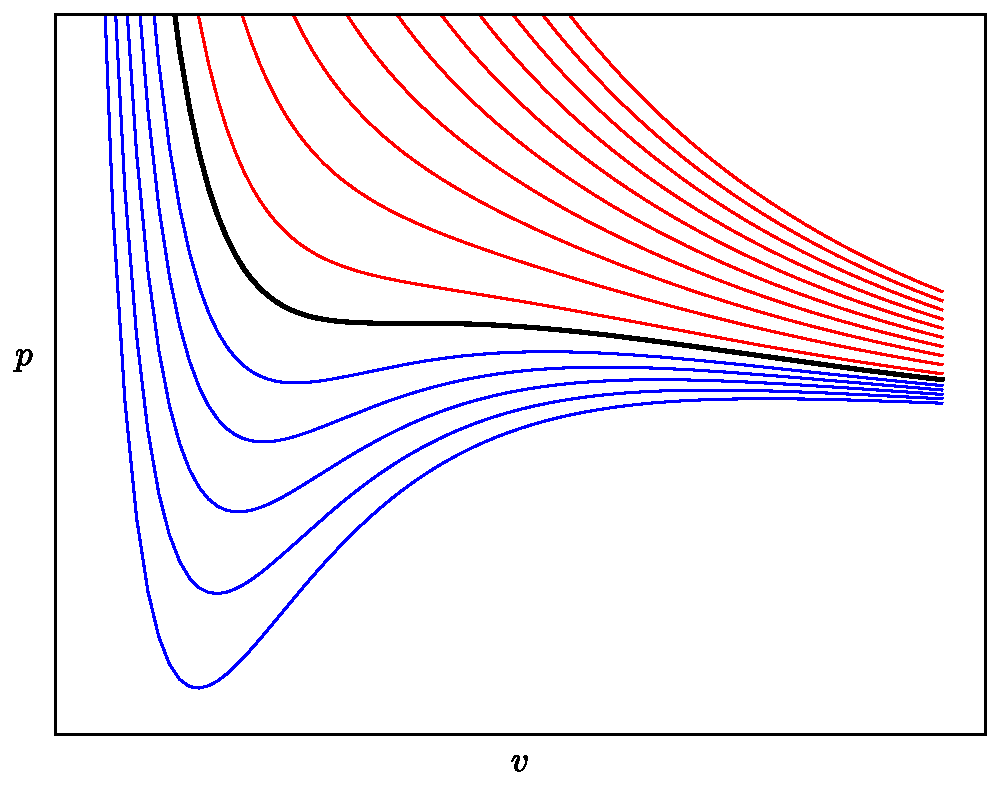
\includegraphics[width=0.75\textwidth]{Pseudopotential/vdW_isoth}
	\caption{Diagrama $p-v$ para la ecuaci\'on de van der Waals. Se destacan las isotermas supercr\'iticas (rojo), cr\'itica (negro) y subcr\'iticas (azul).}
	\label{fig:vdW_isoth}
\end{figure}

La \fig{fig:vdW_isoth} ejemplifica el comportamiento de la ecuaci\'on de van der Waals, donde cada l\'inea corresponde a una isoterma. A medida que la temperatura desciende, las isotermas pasan de un comportamiento similar a un gas ideal, en la esquina superior derecha de la figura, a exhibir un comportamiento en forma de S con un m\'inimo y un m\'aximo locales, en la esquina inferior izquierda. De acuerdo a esas isotermas, existen tres valores de densidad asociadas a una misma presi\'on. Sin embargo, en esa zona de S existe una regi\'on donde $(\partial v / \partial \rho)_T$ es positiva, y por lo tanto se tiene compresibilidad negativa, lo que implica que esa regi\'on es inestable frente a perturbaciones de presi\'on \cite{blundell_concepts_2006}.
La temperatura a partir de la cual se produce este cambio de comportamiento se conoce como temperatura cr\'tica, y es la que se ilustra con una l\'inea m\'as gruesa en la \fig{fig:vdW_isoth}. Esta isoterma presenta un punto de inflexi\'on, conocido como punto cr\'itico, sobre el que se definen propiedades caracter\'isticas de la ecuaci\'on de estado. En particular, analizando las derivadas $(\partial p / \partial v)_T = 0$ y $(\partial^2 p / \partial v^2)_T = 0$, puede encontrarse cu\'al es ese punto cr\'itico, es decir, los valores de presi\'on cr\'itica, volumen molar cr\'itico y temperatura cr\'itica que lo caracterizan:
\begin{equation}
	\begin{gathered}
		p_c = \dfrac{a}{27 b^2} \\
		v_c = 3b \\
		T_c = \dfrac{8 a}{27 R b}
	\end{gathered}
	\label{eq:vdw_param_crit}
\end{equation}

En la \fig{fig:vdW_isoth} se evidencia que para temperaturas por debajo del valor cr\'itico, dos vol\'umenes molares diferentes pueden adoptar el mismo valor de presi\'on en equilibrio $p_0$ (en realidad son 3, pero uno es inestable). Por lo tanto, puede establecerse un estado de coexistencia entre dos fases, l\'iquido y vapor, que compartan igual energ\'ia libre de Gibbs (o equivalentemente potencial qu\'imico). Esta restriccici\'on implica:
\begin{equation}
	\int_{v_l}^{v_g} \left[p_0 - p(v',T)\right] \, \mbox{d} v' = 0,
	\label{eq:maxwell_constr}
\end{equation}
donde $p_0 = p(v_l,T) = p(v_g,T)$. La \eq{eq:maxwell_constr} se conoce como regla de construcci\'on de Maxwell, y determina los vol\'umenes de coexistencia de ambas fases para una determinada temperatura. Si se realiza un cambio de variables adecuado, la \eq{eq:maxwell_constr} puede reescribirse como:
\begin{equation}
	\int_{\rho_g}^{\rho_l} \left[p_0 - p(\rho',T)\right] \dfrac{1}{\rho'} \, \mbox{d} \rho' = 0,
	\label{eq:maxwell_constr_rho}
\end{equation}
donde $p_0 = p(\rho_l,T) = p(\rho_g,T)$. Gr\'aficamente, resolver la regla de Maxwell implica encontrar los vol\'umenes para los que las \'areas sombreadas de la \fig{fig:vdW_Maxwell} sean iguales. 

\begin{figure}[ht]
	\centering
	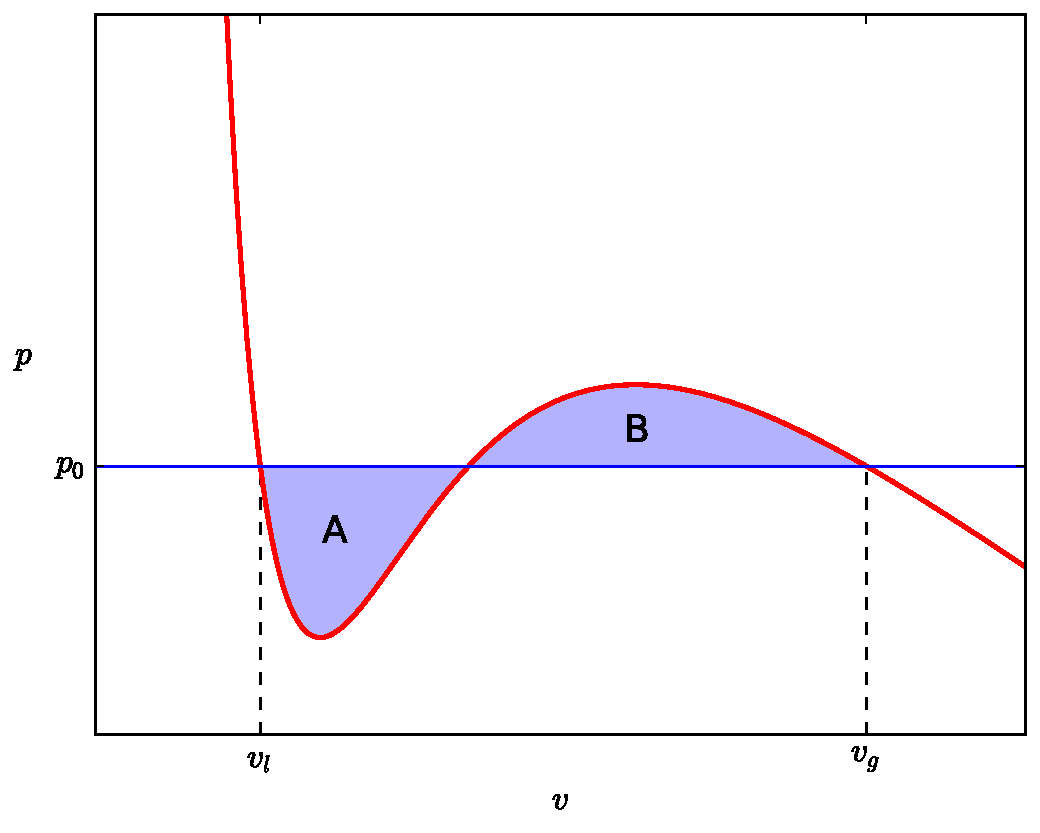
\includegraphics[width=0.75\textwidth]{Pseudopotential/vdW_Maxwell}
	\caption{Ejemplo de aplicaci\'on de la regla de construcci\'on de Maxwell. Dada una isoterma del diagrama $p-v$, los vol\'umenes de coexistencia son aquellos para los que las \'areas $A$ y $B$ son iguales.}
	\label{fig:vdW_Maxwell}
\end{figure}


La regla de construcci\'on de Maxwell aplica a cualquier ecuaci\'on de estado, e impone una restricci\'on termodin\'amica a las simulaciones realizadas con modelos pseudopotential: si se desea recuperar el comportamiento de un fluido regido por una ecuaci\'on de estado, entonces la ``separaci\'on autom\'atica de fases'' propia de esta familia debe ser capaz de reproducir las densidades de equilibrio dadas por la \eq{eq:maxwell_constr}.


\subsubsection*{Otras ecuaciones de estado}

La ecuaci\'on de estado de van der Waals ha alcanzado una notable popularidad, no s\'olo por ser la primera en modelar el comportamiento de gases reales, sino porque a pesar de su simplicidad, permite representar fen\'omenos complejos asociados a la coexistencia y cambio de fase. Sin embargo, esta ecuaci\'on no es la \'unica, ya que se ha creado un amplio abanico de posibilidades en busca de una mejor representaci\'on de diversos tipos de fluidos. A continuaci\'on se detallan dos de las m\'as conocidas, apliamente utilizadas en la literatura de lattice Boltzmann.

\smallskip
\textbf{Carnahan-Starling:}
\begin{equation}
	\begin{gathered}
		p = \rho R T\dfrac{1+b\rho/4+(b\rho/4)^2-(b\rho/4)^3}{(1-b\rho/4)^3} - a\rho^2, \\[2mm]
		p_c = \dfrac{0.07066 \, Ra}{b^2}, \\[2mm]
		T_c = \dfrac{0.37733 \, a}{Rb}, \\[2mm]
		\rho_c = \dfrac{0.5218}{b}
	\end{gathered}
\end{equation}


\textbf{Peng-Robinson:}
\begin{equation}
	\begin{gathered}
		p = \dfrac{\rho R T}{1-b\rho} - \dfrac{a\varphi(\omega,T)\rho^2}{1+2b\rho-(b\rho)^2}, \\[0mm]
		\varphi(\omega,T) = \left[ 1+(0.37464+1.54226\omega-0.26992\omega^2)(1-\sqrt{T/T_c})\right], \\[0mm]
		p_c \approx \dfrac{0.01324 \, a}{b^2}, \\[2mm]
		T_c \approx \dfrac{0.17015 \, a}{Rb}, \\[2mm]
		\rho_c \approx \dfrac{0.253077}{b}
	\end{gathered}
\end{equation}

\red{Poner ac\'a otras propiedades derivadas, como calor latente?}


\subsubsection*{Curvas de coexistencia}

Como se mencion\'o previamente, la regla de construcci\'on de Maxwell permite determinar las densidades de coexistencia en equilibrio para cualquier ecuaci\'on de estado. La determinaci\'on de los l\'imites de esta integral no siempre es sencillo, dado que requiere la aplicaci\'on de un ciclo iterativo, con resultads que dependen de las constantes caracter\'isticas de cada ecuaci\'on de estado. Este c\'alculo, as\'i como la comparaci\'on objetiva entre diferentes ecuaciones de estado, puede simplificarse si se usa el concepto de unidades reducidas \cite{mcquarrie_molecular_1999}:
\begin{equation}
	\rho_r = \rho / \rho_c, \qquad T_r = T / T_c, \qquad p_r = p / p_c,
\end{equation}
donde los sub\'indices $r$ y $c$ denotan propiedades reducidas y cr\'iticas, respectivamente. De acuerdo a la ley de estados correspondientes, las propiedades reducidas deben ser las mismas independientemente del tipo de unidades utilizadas. Por lo tanto, la relaci\'on entre propiedades de coexistencia quedan un\'ivocamente determinadas para cada ecuaci\'on de estado, si se emplean unidades reducidas. De esta forma pueden construirse las llamadas curvas universales de coexistencia, como las mostradas en la \fig{fig:EOS}.

\begin{figure}[ht]
	\centering
	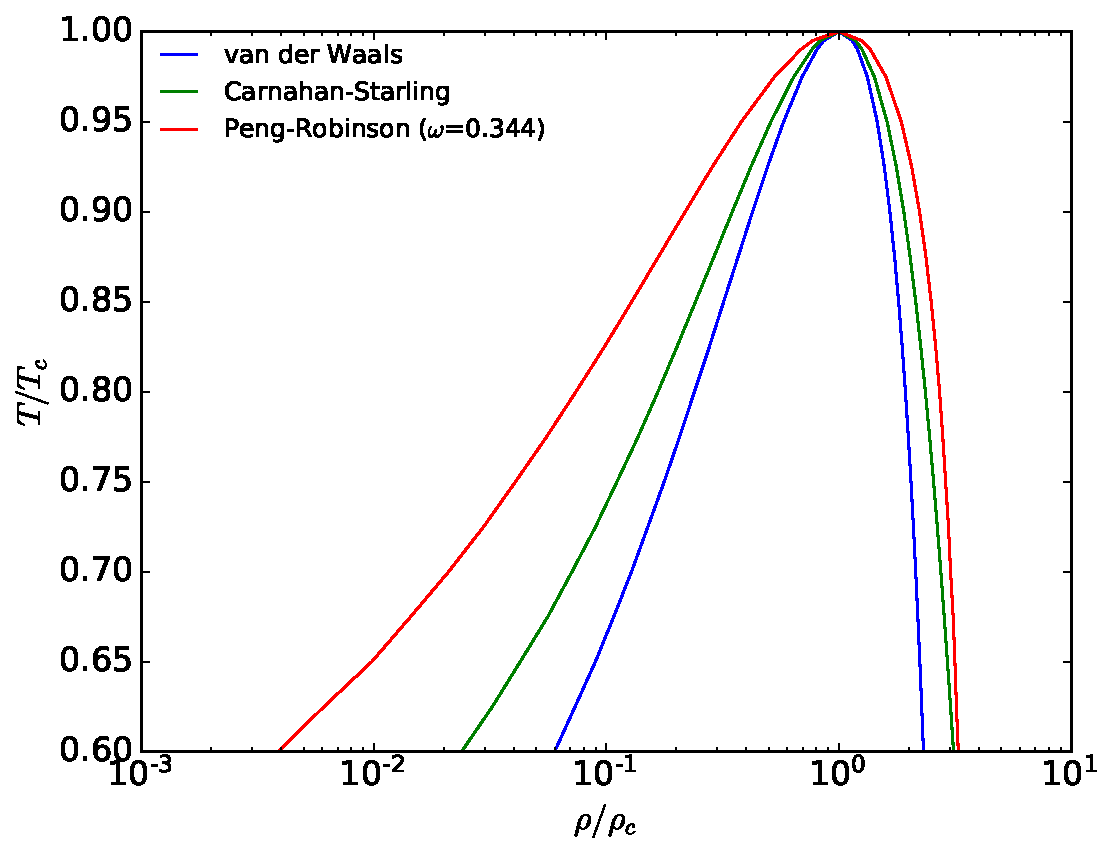
\includegraphics[width=0.75\textwidth]{Pseudopotential/EOS_comp}
	\caption{Densidades de coexistencia, en unidades reducidas, para diferentes ecuaciones de estado.}
	\label{fig:EOS}
\end{figure}





\subsection{Incorporaci\'on de ecuaciones de estado en el potencial de interacci\'on}

La definici\'on de masa efectiva dada por Shan y Chen se aproxima a un valor asint\'otico cuando la densidad es alta, lo que contribuye a evitar el colapso de la fase de mayor densidad y, por lo tanto, contribuir a mejorar la estabilidad de las simulaciones. Sin embargo, el uso de esta expresi\'on fija la ecuaci\'on de estado final, lo que limita la aplicabilidad a diferentes fluidos. En 2006. Yuan y Schaefer \cite{yuan_equations_2006} demostraron que es posible alcanzar relaciones de densidad elevadas en casos est\'aticos si se emplea la masa efectiva introducida por He y Doolen \cite{he_thermodynamic_2002}:
\begin{equation}
	\psi(\rho) = \sqrt{\dfrac{2(p_{EOS} - \rho c_s^2)}{Gc^2}},
\end{equation}
donde $p_{EOS}$ representa una ecuaci\'on de estado no ideal, como Van der Waals, Carnahan-Starling o Peng-Robinson.


\subsection{\red{Adicionales?}}

\red{Podr\'ian ponerse ac\'a ciertos t\'opicos, como la recuperaci\'on de la tensi\'on superficial}






\subsection{La condici\'on de estabilidad mec\'anica y el problema de inconsistencia termodn\'amica}

En el caso sin fuerzas de interacci\'on, a nivel macrosc\'opico se recupera una ecuaci\'on de estado ideal de la forma $p=\rho c_s^2$. Sin embargo, la incorporaci\'on de \ref{eq:f_int} produce una nueva ecuaci\'on de estado dependiente del potencial de interacci\'on:
\begin{equation}
	p = \rho c_s^2 + \dfrac{G}{2} c_s^2 \psi ^2,
\end{equation}
mientras que el tensor de presi\'on $\bm{P}$ queda definido como \cite{he_thermodynamic_2002}:
\begin{equation}
	\nabla \cdot \bm{P} = \nabla \cdot (\rho c_s^2 \bm{I}) - \bm{F}.
	\label{eq:ptens}
\end{equation}

Shan \cite{shan_pressure_2008} demostr\'o que para garantizar un balance mec\'anico exacto, debe considerarse una forma discreta del tensor de presi\'on. En particular, esta expresi\'on puede derivarse a partir de una integral de volumen de la \eq{eq:ptens}:
\begin{equation}
	\int (\nabla \cdot \bm{P}) \, \mbox{d}\Omega = \int \nabla \cdot (\rho c_s^2 \bm{I})\, \mbox{d}\Omega - \int \bm{F} \, \mbox{d}\Omega,
	\label{eq:integral_pres}
\end{equation}
donde $\Omega$ es un volumen cerrado. Si se aplica el teorema de integraci\'on de Gauss a la \eq{eq:integral_pres} resulta
\begin{equation}
	\int \bm{P} \, \mbox{d} \bm{A} = \int \rho c_s^2 \bm{I}\, \mbox{d} \bm{A} - \int \bm{F} \, \mbox{d}\Omega,
\end{equation}
donde $\mbox{d} \bm{A}$ es un diferencial de \'area. En forma discreta, esta integral puede escribirse como
\begin{equation}
	\sum \bm{P} \cdot \bm{A} = \sum \rho c_s^2 \bm{I} \cdot \bm{A} - \sum \bm{F}.
\end{equation}

Por lo tanto, el tensor de presi\'on finalmente puede escribirse como:
\begin{equation}
	\bm{P} = \rho c_s^2 \bm{I} + \dfrac{G}{2}\psi(\bm{x}) \sum_{\alpha=1}^N w(|\bm{e}_{\alpha}|^2)\psi(\bm{x}+\bm{e}_{\alpha})\bm{e}_{\alpha}\bm{e}_{\alpha}.
	\label{eq:ptens_shan}
\end{equation}

En el caso de considerar s\'olo interacciones con los vecinos cercanos (ubicados a una distancia m\'axima de $\sqrt{2}$ o $\sqrt{3}$ unidades de grilla en 2 o 3 dimensiones respectivamente), la expansi\'on en serie de Taylor de la \eq{eq:ptens_shan} resulta:
\begin{equation}
	\bm{P} = \left( \rho c_s^2 + \dfrac{G c^2}{2} \psi^2 + \dfrac{G c^4}{12} \psi \nabla^2 \psi \right) \bm{I} + \dfrac{G c^4}{6} \psi \nabla \nabla \psi.
	\label{eq:ptens_shan_taylor}	
\end{equation}

La \eq{eq:ptens_shan_taylor} puede usarse para determinar la presi\'on normal a una interfase plana
\begin{equation}
	P_n = \rho c_s^2 + \dfrac{G c^2}{2} \psi^2 + \dfrac{G c^4}{12} \left[ \alpha \left( \dfrac{d\psi}{dn} \right)^2 + \beta \psi \dfrac{d^2 \psi}{dn^2} \right],
	\label{eq:ptens_shan_plane}	
\end{equation}
donde $n$ denota la direcci\'on normal a la interfase, y en el caso de interacci\'on de vecinos cercanos se cumple $\alpha = 0$ y $\beta = 3$. Por lo tanto, tomando como base la \eq{eq:ptens_shan_plane} y considerando que en equilibrio la presi\'on $P_n$ debe ser igual a la presi\'on est\'atica en el seno del fluido \cite{shan_pressure_2008}, puede derivarse la condici\'on de estabilidad mec\'anica:
\begin{equation}
	\int_{\rho_g}^{\rho_l} \left( p_0 - \rho c_s^2 - \dfrac{Gc^2}{2} \psi^2 \right) \dfrac{\psi'}{\psi^{1+\varepsilon}} \, \mbox{d}\rho = 0,
\end{equation}
donde $\psi' = d\psi / d\rho$, $\varepsilon=-2\alpha/\beta$ y $p_0=p(\rho_l)=p(\rho_g)$. De esta forma, puede verse que la condici\'on de estabilidad mec\'anica conduce a densidades de coexistencia que en general ser\'an diferentes a las establecidas por la construcci\'on de Maxwell (\eq{eq:maxwell_constr_rho}), ya que si el potencial de interacci\'on satisface la propuesta de He y Doolen, entonces en general no puede cumplirse que $\psi' / \psi^{1+\varepsilon} \propto 1/\rho^2$. Esta incompatibilidad se conoce con el nombre de inconsistencia termodin\'amica.


\section{El modelo isot\'ermico de Li et al.}

Los modelos pseudopotential proveen una alternativa sencilla y eficiente para poder simular num\'ericamente el comportamiento de flujos m\'ultif\'asicos. Esta simplicidad, sin embargo, tiene su precio: las primeras versiones encontraron r\'apidamente un l\'imite de aplicabilidad, no s\'olo por el problema de inconsistencia termodin\'amica, sino por la fuerte presencia de corrientes esp\'ureas en las interfases, a\'un en problemas est\'aticos o cuasi-est\'aticos. Esta combinaci\'on de factores llev\'o a que durante mucho tiempo, el uso del m\'etodo pseudopotential se limitase a la resoluci\'on de problemas con baja relaci\'on de densidades y bajo n\'umero de Reynolds.

El camino hacia versiones m\'as estables fue forj\'andose con trabajos que buscan identificar el origen de estas inestabilidades num\'ericas, junto con mecanismos te\'oricos para remediarlas (al menos parcialmente). A modo de ejemplo es interesante destacar el trabajo de Shan \cite{shan_analysis_2006}, en el cu\'al se describe a las corrientes esp\'ureas como un fen\'omeno que tiene lugar cerca de la interfase de una burbuja estacionaria, y en el cual se produce un flujo peque\~no pero finito alrededor de la misma. El patr\'on de este flujo presenta la misma simetr\'ia que la grilla subyacente, y su magnitud es inversamente proporcional a la viscosidad del fluido simulado. Shan demostr\'o que existe una conexi\'on directa entre este fen\'omeno y la falta de isotrop\'ia en ciertos operadores diferenciales discretos, en particular el empleado en la reprentaci\'on discreta de la fuerza de interacci\'on (\eq{eq:f_int}). Denotando a los tensores 
\begin{equation}
	E^{(n)}_{i_1i_2\ldots i_n} = \sum_{\alpha}w(|\bm{e}_{\alpha}|^2)(\bm{e}_{\alpha})_{i_1} \cdots (\bm{e}_{\alpha})_{i_n},
\end{equation}
entonces puede escribirse el gradiente de una funci\'on $f$ como:
\begin{equation}
	\sum_{\alpha}w(|\bm{e}_{\alpha}|^2) f(\bm{x}+\bm{e}_{\alpha})\bm{e}_{\alpha}=(\nabla f)\cdot \bm{E}^{(2)} + \dfrac{1}{3!}(\nabla^{(3)} f)\cdot \bm{E}^{(4)} + \dfrac{1}{5!}\nabla^{(5)} f)\cdot \bm{E}^{(6)} + \ldots.
\end{equation}
Por lo tanto, la mejor aproximaci\'on a $\nabla f$ se logra si todos los tensores $\bm{E}^{(n)}$ son isotr\'opicos, aunque este requisito no puede alcanzarse debido a que existe un n\'umero finito de  velocidades discretas. Sin embargo, Shan demostr\'o que pueden encontrarse conjuntos adecuados de pesos $\{ w(\bm{e}_{\alpha})\}$ que mejoran notoriamente la isotrop\'ia de la aproximaci\'on, y por lo tanto, reducen la magnitud de las corrientes esp\'ureas.

Dentro de un contexto similar al presentado por Shan, Sbragaglia y sus colaboradores adoptaron una nueva expresi\'on para la fuerza de interacci\'on en la que se tienen en cuenta las interacciones de rango medio, es decir, se consideran aquellos nodos que no son vecinos inmediatos \cite{sbragaglia_generalized_2007}:
\begin{equation}
	\bm{F}_i = -c_s^2 \psi(\bm{x}) \sum_{\alpha} w(|\ea|^2) \left[G_1 \psi(\xplus)  + G_2 \psi(\bm{x}+2\bm{e}_{\alpha}) \right]
	\label{eq:fi_sbragaglia}
\end{equation}

Usando esta aproximaci\'on, Sbragaglia et al. demostraron anal\'iticamente que, para una interfase plana, la \eq{eq:fi_sbragaglia} conduce a una tensi\'on superficial que depende de las constantes $G_1$ y $G_2$, y por lo tanto es ajustable. Por otro lado, la extensi\'on del stencil en el c\'alculo de la fuerza de interacci\'on permite reducir el espesor de la interfase y elevar la relaci\'on de densidades en simulaciones estacionarias.

\red{poner cambios en esquemas de fuerzas}

Las contribuciones de Shan y Sbragaglia ilustran la evoluci\'on que ha sufrido (y que contin\'ua experimentando) el modelo original de Shan y Chen buscando mejorar la precisi\'on, estabilidad y aplicabilidad del m\'etodo. En pocas palabras, estos esfuerzos pueden describirse como un compromiso entre la aplicaci\'on adecuada de la fuerza de interacci\'on, y la preservaci\'on de un algoritmo eficiente y de sencilla implementaci\'on.

\red{Mencionar que son modelos 2D}
Entre las alternativas pseudopotential m\'as recientes, el modelo introducido por Li et al. \cite{li_lattice_2013} contiene esas caracter\'isticas de equilibrio antes mencionadas. En esta propuesta se hace uso de un operador de colisi\'on MRT, de modo que la \lbe{} vectorial resulta:
\begin{equation}
	\bm{f} (\bm{x} + \bm{e}\delta_t, t+\delta_t) = \bm{M}^{-1}\left[ \bm{m} - \bm{\Lambda}(\bm{m} - \feq{m})  + \delta_t \left( \bm{I} - \dfrac{\bm{\Lambda}}{2} \bar{\bm{S}} \right) \right].
	\label{eq:lbe_li}
\end{equation}

Como se mostr\'o en el \red{Cap\'itulo 2}, $\bm{m} = \bm{Mf}$ corresponde a la proyecci\'on de la funci\'on de distribuci\'on $\bm{f}$ en el espacio de momentos, y $\feq{m} = \bm{M}\feq{f}$ a la transformaci\'on de la distribuci\'on de equilibrio. En este caso se usa la matriz de transformaci\'on y funci\'on de equilibrio est\'andar (\red{Ecuaciones XX y YY respectivamente}), de modo que la distribuci\'on de equilibrio en el espacio de momentos puede escribirse como:
\begin{equation}
\feq{m} = \rho (1, -2+3|\bm{u}|^2, 1-3|\bm{u}|^2, u_x, -u_x, u_y, -u_y, u_x^2-u_y^2, u_xu_y)^T.
\end{equation}

La matriz $\bm{\Lambda}$ corresponde a una matriz diagonal cuyos componentes se denotan mediante
\begin{equation}
	\bm{\Lambda}=diag(\tau_{\rho}^{-1},\tau_{e}^{-1},\tau_{\zeta}^{-1},\tau_{j}^{-1},\tau_{q}^{-1},\tau_{j}^{-1},\tau_{q}^{-1},\tau_{\nu}^{-1},\tau_{\nu}^{-1}).
\end{equation}

En este modelo, las cantidades macrosc\'opicas conservadas corresponden a la densidad y velocidad, y pueden recuperarse siguiendo el esquema de fuerzas de Guo:
\begin{equation}
	\begin{gathered}
		\rho = \sum_{\alpha} f_{\alpha}, \\
		\rho \bm{u} = \sum_{\alpha} \bm{e}_{\alpha} f_{\alpha} + \dfrac{\delta_t}{2} \bm{F},
	\end{gathered}
\end{equation}

donde $\bm{F}$ corresponde a la fuerza total actuando sobre el sistema. En la mayor\'ia de los casos analizados, $\bm{F}$ contiene una componente volum\'etrica ($\bm{F}_b$) y otra asociada al potencial de interacci\'on, de modo que se utiliza $\bm{F} = \bm{F}_b + \bm{F}_i$.

Siguiendo la idea detallada en un trabajo anterior de Li y sus colaboradores \cite{li_forcing_2012}, la fuerza de interacci\'on tambi\'en debe incorporarse durante la colisi\'on a trav\'es del t\'ermino de fuente $\bar{\bm{S}}$, definido en el espacio de momento como:
\begin{equation}
 \bar{\bm{S}} = 
 \left[ 
 	\begin{array}{c} 
 		0	\\
 		6 \bm{u} \cdot \bm{F} + \dfrac{12\sigma |\bm{F}_i|^2}{\psi^2 \delta_t (\tau_e-0.5)} \\
 		-6 \bm{u} \cdot \bm{F} - \dfrac{12\sigma |\bm{F}_i|^2}{\psi^2 \delta_t (\tau_{\zeta}-0.5)} \\
 		F_x \\
 		-F_x \\
 		F_y \\
 		-F_y \\
 		2(u_xF_x - u_yF_y) \\
 		(u_xF_y + u_yF_x)
 	\end{array} 
 \right]
 \label{eq:s_li}
\end{equation}

La principal novedad del modelo de Li consiste en la incorporaci\'on de t\'erminos adicionales en las componentes 1 y 2 de la \eq{eq:s_li}, que dependen linealmente de un par\'ametro libre $\sigma$. En particular, aplicando la expansi\'on de Chapman-Enskog a las Ecs.~(\ref{eq:lbe_li})-(\ref{eq:s_li}) se demuestra que las variables macrosc\'opicas satisfacen:
\begin{equation}
	\dfrac{\partial (\rho \bm{u})}{\partial t} + \nabla \cdot (\rho \bm{uu}) = -\nabla \cdot (\rho c_s^2 \bm{I}) + \nabla \cdot \bm{\Pi} + \bm{F} - 2G^2 c^4 \sigma \nabla \cdot (|\nabla \psi|^2 \bm{I}),
\end{equation}
de modo que el nuevo tensor de presi\'on satisface:
\begin{equation}
	\nabla \cdot \bm{P} = \nabla \cdot (\rho c_s^2 \bm{I}) - \bm{F} + 2G^2 c^4 \sigma \nabla \cdot (|\nabla \psi|^2 \bm{I})
\end{equation}
y, de acuerdo a la metodolog\'ia de Shan \cite{shan_pressure_2008}, puede escribirse como:
\begin{equation}
	\bm{P} = \bm{P}_{\mbox{orig}} + 2G^2 c^4 \sigma (|\nabla \psi|^2 \bm{I}),
\end{equation}
donde $\bm{P}_{\mbox{orig}}$ corresponde al tensor original definido por la \eq{eq:ptens_shan_taylor}. De este resultado se desprende que la nueva diferencia de presi\'on a trav\'es de una interfase plana corresponde a:
\begin{equation}
	P_n = \rho c_s^2 + \dfrac{G c^2}{2} \psi^2 + \dfrac{G c^4}{12} \left[ (\alpha+24G\sigma) \left( \dfrac{d\psi}{dn} \right)^2 + \beta \psi \dfrac{d^2 \psi}{dn^2} \right],
\end{equation}
y, por lo tanto, $\varepsilon=-2(\alpha + 24 G \sigma)/\beta$. De esta manera, la condici\'on de estabilidad mec\'anica ($\varepsilon$) ya no queda determinada s\'olo por el conjunto de velocidades de grilla, sino que puede ajustarse a trav\'es del par\'ametro libre $\sigma$. Esta nueva aproximaci\'on sigue sin cumplir formalmente con la incompatibilidad planteada por la inconsistencia termodin\'amica, pero como se muestra en las secciones siguientes, permite alcanzar una excelente representaci\'on de las curvas de coexistencia para un amplio rango de temperaturas.

%\chapter{Transferencia de calor en flujo multif\'asico bidimensional}
\label{chap:modelo2D}

La simulaci\'on de flujos multif\'asicos isot\'ermicos con LB comenz\'o pr\'acticamente con el origen del m\'etodo, y el desarrollo continuo de modelos ha permitido aplicar esta t\'ecnica a un amplio abanico de problemas. Sin embargo, a pesar del \'exito de LB en \'este \'area, la simulaci\'on de transferencia de calor contin\'ua como un t\'opico abierto y en pleno desarrollo.

En el presente cap\'itulo se introduce un nuevo modelo para simular la transferencia de calor en flujos multif\'asicos, basado en una \lbe{} que permite recuperar adecuadamente una ecuaci\'on de energ\'ia consistente termodin\'amicamente con la aproximaci\'on pseudopotencial. El nuevo modelo, desarrollado formalmente para una grilla D2Q9, es validado con un conjunto de experimentos num\'ericos con soluci\'on anal\'itica. Aspectos tradicionales de la propuesta, como consistencia e independencia de grilla, son analizados a partir de la simulaci\'on de generaci\'on de burbujas sobre una superficie horizontal calefaccionada. Los principales resultados de este an\'alisis se encuentran publicados en \cite{fogliatto_assessment_2021}.


\section{Transporte de calor en lattice Boltzmann}

En general, los modelos LB existentes que permiten simular transferencia de calor en flujos multif\'asicos pueden clasificarse en tres categor\'ias principales: modelos de velocidad m\'ultiple (\emph{multi-speed}), modelos h\'ibridos (\emph{hybrid}) y modelos con dos funciones de distribuci\'on (\emph{double-distribution}). En el primer caso, las propiedades macrosc\'opicas del fluido como densidad, velocidad y temperatura, se obtienen a partir de los momentos cero, primero y segundo de una \'unica funci\'on de distribuci\'on \cite{succi_lattice_2018,alexander_lattice_1993}. A pesar que estos modelos cuentan con un s\'olido fundamento te\'orico, su difusi\'on es limitada, ya que t\'ipicamente emplean un conjunto de velocidades mayor que el correspondiente modelo isot\'ermico. Adem\'as, suelen incorporar t\'erminos de mayor orden en la \edf{} y est\'an restringidos a la simulaci\'on de un fluido con n\'umero de Prandtl fijo.

Estas limitaciones intr\'insecas de los modelos de velocidad m\'ultiple motivaron el desarrollo de otro tipo de modelos t\'ermicos, donde se introduce un acoplamiento expl\'icito entre un esquema isot\'ermico para las ecuaciones hidrodin\'amicas, y una t\'ecnica alternativa para el transporte de energ\'ia. Los modelos h\'ibridos \cite{dong_numerical_2012,li_lattice_2015}, por un lado, aprovechan la discretizaci\'on del dominio asociada a la ecuaci\'on hidrodin\'amica, y hacen uso de un esquema c\'asico de diferencias finitas para encontrar la soluci\'on de la ecuaci\'on de energ\'ia correspondiente. Por otro lado, los modelos con dos funciones de distribuci\'on introducen una segunda \lbe{} para recuperar la ecuaci\'on macrosc\'opica deseada.

Los esquemas de doble \fdp{} heredan las principales ventajas de LB, como simplicidad del algoritmo y elevada eficiencia computacional. Sin embargo, tambi\'en presentan las limitaciones comunes derivadas de la representaci\'on de ecuaciones escalares de advecci\'on-difusi\'on \cite{markus_simulation_2011, huang_modified_2014, li_improved_2017, huang_numerical_2011, li_effect_2014, huang_multiphase_2015}. En este tipo de ecuaciones hay una \'unica cantidad conservada (por ejemplo temperatura), de modo que se relajan las condiciones de isotrop\'ia y es posible, en teor\'ia, emplear distribuciones de equilibrio lineales (en la velocidad del fluido) o conjuntos de velocidades reducidos. Sin embargo, la expansi\'on de Chapman-Enskog de estos esquemas muestra que existen t\'erminos no deseados que se recuperan inevitablemente en las ecuaciones macrosc\'opicas \cite{kruger_lattice_2017, huang_modified_2014, huang_numerical_2011}, y en el caso de los modelos para flujo multif\'asico con transferencia de calor, estos t\'erminos producen fuentes de calor adicionales que dependen del potencial de interacci\'on o de derivadas temporales de la velocidad del fluido.

Un ejemplo t\'ipico de estas restricciones puede analizarse con el uso de una \lbe{} con operador de colisi\'on SRT destinada a recuperar una ecuaci\'on de advecci\'on-difusi\'on de un escalar pasivo $\phi$:
\begin{equation}
	\dfrac{\partial \phi}{\partial t} + \nabla \cdot (\phi \bm{u}) = \nabla \cdot (k \nabla \phi),
	\label{eq:adv_dif_phi}
\end{equation}
donde $k$ es una constante de difusi\'on. En este caso, si se utiliza un esquema cl\'asico de LB para una \fdp{} $\bm{g}$, es decir:
\begin{equation}
	\begin{gathered}
		g_{\alpha}(\bm{x}+\bm{e}_{\alpha}\delta_t, t+\delta_t) - g_{\alpha}(\bm{x},t) = -\dfrac{1}{\tau} \left[ g_{\alpha}(\bm{x},t) - g^{eq}_{\alpha}(\bm{x},t) \right], \\[2mm]
		g_{\alpha}^{eq} = w_i \phi \left[ 1 + \dfrac{e_{i\alpha}u_{\alpha}}{c_s^2} + \dfrac{u_{\alpha}u_{\beta}(e_{i\alpha}e_{i\beta}-c_s^2\delta_{\alpha\beta})}{2c_s^4} \right], \\[2mm]
		\phi = \sum_{\alpha} g_{\alpha},
	\end{gathered}
\end{equation}
entonces puede demostrarse que la ecuaci\'on macrosc\'opica recuperada para $\phi$ satisface:
\begin{equation}
	\dfrac{\partial \phi}{\partial t} + \nabla \cdot (\phi \bm{u}) = \nabla \cdot \left\{ \delta_t(\tau - 0.5) \left[ \dfrac{\partial (\phi\bm{u})}{\partial t} + \nabla \cdot (\phi \bm{uu}) + c_s^2 \nabla \phi\right]\right\}.
	\label{eq:adv_dif_phi_rec}
\end{equation}

En este caso, el coeficiente de difusi\'on recuperado est\'a dado por $k=c_s^2 \delta_t(\tau-0.5)$. A diferencia de la \eq{eq:adv_dif_phi}, la \eq{eq:adv_dif_phi_rec} contiene un t\'ermino de desviaci\'on dado por $\nabla \cdot \{ \delta_t(\tau - 0.5) [ \partial_t (\phi\bm{u}) + \nabla \cdot (\phi \bm{uu}) ]\}$, que puede anularse completamente s\'olo en aquellos casos con perfiles de velocidad especiales, como $\bm{u}=const$, $\bm{u}=[u_x(y),0]$, $\bm{u}=[0,u_y(x)]$, etc. 

Ejemplos similares pueden encontrarse dentro de los modelos \pp{} \cite{li_effect_2014}. En ciertas aplicaciones se desea recuperar una ecuaci\'on macrosc\'opica de la forma:
\begin{equation}
	\dfrac{\partial (\rho c_v T)}{\partial t} + \nabla \cdot (\rho c_v T \bm{u}) = \nabla \cdot (\lambda \nabla T),
\end{equation}
donde $\lambda$ es la conductividad t\'ermica y $c_v$ el calor espec\'ifico a volumen constante. En este caso el esquema usual consiste en utilizar una \lbe{} \pp{} est\'andar para la funci\'on de distribuci\'on $\bm{f}$, asociada a las ecuaciones hidrodin\'amicas, mientras que este esquema tambi\'en puede utilizarse para una segunda distribuci\'on $\bm{g}$, con $g^{eq}_{\alpha} = c_v T f^{eq}_{\alpha}$ y $\sum g_{\alpha} = \rho c_v T$. Nuevamente, la expansi\'on de Chapman-Enskog demuestra que la ecuaci\'on macrosc\'opica recuperada resulta:
\begin{equation}
	\dfrac{\partial (\rho c_v T)}{\partial t} + \nabla \cdot (\rho c_v T \bm{u}) = \nabla \cdot \left(\lambda \nabla T + \dfrac{\lambda}{p}T\bm{F} \right),
	\label{eq:e_macro_F}
\end{equation}
es decir, aparece un t\'ermino no deseado asociado a la fuerza total de la ecuaci\'on de impulso. Si estos t\'erminos son identificados, como en este caso, entonces pueden ser compensados expl\'icitamente:
\begin{equation}
	g_{\alpha}(\bm{x}+\bm{e}_{\alpha}\delta_t, t+\delta_t) - g_{\alpha}(\bm{x},t) = -\dfrac{1}{\tau} \left[ g_{\alpha}(\bm{x},t) - g^{eq}_{\alpha}(\bm{x},t) \right] + \delta_t C_{\alpha}(\bm{x},t),
\end{equation}
donde $C_{\alpha}$ es un t\'ermino de correcci\'on:
\begin{equation}
	C_{\alpha} = \left( 1-\dfrac{1}{2\tau} \right)\omega_{\alpha}c_v T \dfrac{\bm{e}_{\alpha} \cdot \bm{F}}{c_s^2}.
\end{equation}

\nomenclature[N]{$\lambda$}{Conductividad t\'ermica}
\nomenclature[N]{$c_v$}{Calor espec\'ifico a volumen constante}

En definitiva, los modelos de doble \fdp{} resultan atractivos, ya que permiten conservar la elegancia y simpleza propia de lattice Boltzmann, mientras que aportan una mayor flexibilidad en el tipo de ecuaciones macrosc\'opicas que pueden recuperarse. Sin embargo, si se desea incrementar la aplicabilidad de estos modelos hacia problemas m\'as complejos, es necesario desarrollar un mecanismo natural para eliminar los t\'erminos no deseados en la ecuaci\'on macrosc\'opica recuperada. Por lo tanto, siguiendo este objetivo primario, en la secci\'on siguiente se introduce un modelo alternativo que permite remediar satisfactoriamente estas limitaciones.


\section{Ecuaci\'on de energ\'ia con operador MRT}
El modelo \pp{} de Li ha sido extensamente validado en la bibliograf\'ia, donde se ha demostrado que puede utilizarse exitosamente en la simulaci\'on de flujos multif\'asicos bidimensionales, con $Re$ moderados y relaci\'on de densidades elevadas (hasta $\rho_l / \rho_g \sim 750$). Adicionalmente, los resultados de la simulaci\'on de un fluido vdW mostrados en el \chap{chap:isot} y en \cite{fogliatto_simulation_2019}, sugieren que el modelo es capaz de incorporar adecuadamente fuerzas externas sin afectar la correcci\'on sobre la inconsistencia termodin\'amica. El an\'alisis de convergencia en malla, que en este contexto se traduce en un incremento de unidades de grilla conservando par\'ametros adimensionales, muestra que es posible alcanzar una precisi\'on adecuada en la reproducci\'on de interfases. Sin embargo, si se desea expandir su uso hacia la simulaci\'on de flujos multif\'asicos con transferencia de calor y cambio de fase, entonces es necesario proveer un nuevo esquema para cuantificar adecuadamente el transporte de energ\'ia.

Dentro del contexto de modelos \pp{}, donde se consideran fluidos cuya presi\'on termodin\'amica se encuentra gobernada por una \eos{}, la ecuaci\'on de energ\'ia macrosc\'opica debe seguir una forma particular. Tomando como base un balance local de entrop\'ia, y despreciando efectos de disipaci\'on viscosa, M\'arkus y H\'azi derivaron una ecuaci\'on macrosc\'opica para la energ\'ia, representada por medio de la temperatura \cite{markus_simulation_2011}:
\begin{equation}
	\dfrac{\partial T}{\partial t} + \bm{u} \cdot \nabla T = \dfrac{1}{\rho c_v} \nabla \cdot(\lambda \nabla T) - \dfrac{T}{\rho c_v} \left( \dfrac{\partial p_{EOS}}{\partial T} \right)_{\rho} \nabla \cdot \bm{u},
	\label{eq:markus_orig}
\end{equation}
La \eq{eq:markus_orig} consiste en una ecuaci\'on de advecci\'on-difusi\'on para $T$, con un t\'ermino de fuente asociado al trabajo de compresi\'on. En las secciones siguientes se considerar\'a que la difusividad t\'ermica $\chi = \lambda/(\rho c_v)$ y el calor espec\'ifico $c_v$ son constantes en cada fase, de modo que la \eq{eq:markus_orig} puede reescribirse como:
\begin{equation}
	\dfrac{\partial T}{\partial t} + \nabla \cdot (\bm{u} T) = \chi \nabla^2 T  + \dfrac{\chi}{\rho} \nabla T \cdot \nabla \rho + T \left[ 1 - \dfrac{1}{\rho c_v} \left( \dfrac{\partial p_{EOS}}{\partial T} \right)_{\rho} \right] \nabla \cdot \bm{u}
	\label{eq:markus}
\end{equation}
\nomenclature[N]{$\chi$}{Difusividad t\'ermica}

Esta aproximaci\'on, si bien implica una p\'erdida de generalidad, facilita el desarrollo del esquema LB. Por otro lado, como se describe en las secciones siguientes,  la forma original de la ecuaci\'on puede recuperarse usando t\'erminos de fuente adecuados. 

Para satisfacer esta restricci\'on es posible partir del an\'alisis sobre la simulaci\'on de ecuaciones de advecci\'on-difus\'on llevado a cabo por Huang y colaboradores \cite{huang_modified_2014, huang_numerical_2011, huang_lattice_2015}: la recuperaci\'on de una ecuaci\'on escalar usando una \lbe{} con operador de colisi\'on MRT permite combinar aquellos momentos responsables de los t\'erminos no deseados. Si esta interacci\'on se lleva a cabo de forma inteligente, entonces es posible lograr la supresi\'on de componentes espec\'ificos dentro de las escalas de expansi\'on analizadas. Por otro lado, como se desea recuperar un t\'ermino de fuente, \'este debe incorporarse al esquema sin que se reproduzcan derivadas convectivas de dicha fuente \cite{cheng_introducing_2008}, lo que fuerza a la incorporaci\'on de un t\'ermino de fuente impl\'icito. Combinando estas ideas, una \lbe{} adecuada para recuperar la \eq{eq:markus} resulta:

\begin{equation}
	\begin{aligned}
		\tilde{\bm{g}}(\bm{x} + \bm{e} \delta_t, t+\delta_t) &=
		\tilde{\bm{g}}(\bm{x}, t) - (\bm{M}^{-1}Q\bm{M}) \left[ \tilde{\bm{g}}(\bm{x}, t) - \tilde{\bm{g}}^{eq}(\bm{x}, t) \right] \\
		&  + \dfrac{\delta_t}{2} \hat{\bm{\Gamma}}(\bm{x},t) + \hat{\bm{\Gamma}}(\bm{x} +\bm{e}\delta_t,t + \delta_t),
	\end{aligned}
	\label{eq:g_tilde_2d}	
\end{equation}

\begin{equation}
	\sum_{\alpha} \tilde{g}_{\alpha} = T.
\end{equation}

Siguiendo la notaci\'on usada previamente para las \lbe{} con operador MRT, la componente $\alpha$-\'esima del miembro izquierdo de la \eq{eq:g_tilde_2d} corresponde  a $\tilde{g}_{\alpha}(\bm{x}+\bm{e}_{\alpha}\delta_t)$, y $\bm{M}$ a la matriz de transformaci\'on al espacio de momentos (\eq{eq:MRT_M_D2Q9}).  En este caso, $\bm{Q}$ corresponde a una matriz de coeficientes relajaci\'on y $\hat{\bm{\Gamma}} = \bm{M}^{-1}\bm{\Gamma}$ a un t\'ermino de fuente en el espacio de poblaciones. Como la \eq{eq:g_tilde_2d} contiene una fuente \'implicita, puede transformarse usando:
\begin{equation}
	g_{\alpha}(\bm{x},t) = \tilde{g}_{\alpha} (\bm{x},t) - \dfrac{\delta_t}{2} \hat{\Gamma}_{\alpha}(\bm{x},t),
	\label{eq:g_tilde_tranf_2d}
\end{equation}
de modo que el momento de orden cero de $\bm{g}$ resulta:
\begin{equation}
	\begin{aligned}
		T &= \sum_{\alpha} \tilde{g}_{\alpha} \\
		  &= \sum_{\alpha} g_{\alpha} + \dfrac{\delta_t}{2} \sum_{\alpha} \tilde{\Gamma}_{\alpha} \\
		  &= \sum_{\alpha} g_{\alpha} + \dfrac{\delta_t}{2} \Gamma_0
	\end{aligned}
	\label{eq:T_macro_2d}
\end{equation}

En la \eq{eq:T_macro_2d} se utiliza que la primera fila de $\bm{M}$ corresponde a $\bm{M}_0 = (1, \cdots ,1)$, de forma que $T$ puede obtenerse usando la distribuci\'on $\bm{g}$ y la primera componente de la fuente en el espacio de momentos. La \eq{eq:g_tilde_2d} puede reescribirse usando la \eq{eq:g_tilde_tranf_2d} como:
\begin{equation}
	\bm{g}(\bm{x} + \bm{e} \delta_t, t+\delta_t) = \bm{M}^{-1} \left[ \bm{n} - \bm{Q}(\bm{n} - \feq{n}) + \delta_t \left( \bm{I}-\dfrac{\bm{Q}}{2}\right) \bm{\Gamma}\right],
	\label{eq:g_model_2d}
\end{equation}
donde $\bm{n} = \bm{Mg}$ y se omiti\'o la dependencia $(\bm{x},t)$ por claridad. La determinaci\'on de la ecuaci\'on macrosc\'opica  recuperada puede hacerse mediante una expansi\'on de Chapman-Enskog, considerando las ideas expuestas en la \se{sec:chapman}. En primer lugar, es necesario reescribir el t\'ermino izquierdo de la \eq{eq:g_model_2d} empleando un desarrollo de Taylor para cada componente, es decir:
\begin{equation}
	g_{\alpha}(\bm{x}+\bm{e}_{\alpha}\delta_t,t+\delta_t) = \sum_{k=0}^{\infty} \dfrac{1}{k!}\delta_t^k D_{\alpha}^{k} \, g_{\alpha} \sim g_{\alpha} + \delta_t D_{\alpha} g_{\alpha} + \dfrac{1}{2}\delta_t^2 D_{\alpha}^2g_{\alpha},
	\label{eq:taylor_gral}
\end{equation}
donde $D_{\alpha} = \partial_t + \bm{e}_{\alpha} \cdot \nabla=\partial_t + e_{\alpha \beta} \partial_{\beta}$. Para escribir la \eq{eq:taylor_gral} en forma vectorial, es necesario definir las matrices diagonales $\bm{E}_{\beta} = diag(e_{0\beta} \cdots e_{q-1\beta})$ y $\bm{\nabla}_{\beta} = \partial_{\beta} \bm{I}$, de modo que la \eq{eq:taylor_gral} puede transformarse como:
\begin{equation}
	\bm{g}(\bm{x}+\bm{e}\delta_t. t+\delta_t) = \bm{g} 
	+ \delta_t\left( \dfrac{\partial}{\partial t} \bm{I} + \bm{E}_{\beta}\bm{\nabla}_{\beta} \right) \bm{g}
	+ \dfrac{\delta^2_t}{2} \left( \dfrac{\partial}{\partial t} \bm{I} + \bm{E}_{\beta}\bm{\nabla}_{\beta} \right)^2 \bm{g}.
	\label{eq:taylor_vec}
\end{equation}

Reemplazando la \eq{eq:taylor_vec} en la \eq{eq:g_model_2d} y multiplicando ambos miembros por $\bm{M}$, se obteniene una \lbe{} desarrollada en torno a $(\bm{x},t)$:
\begin{equation}
	\begin{aligned}
	\delta_t \bm{M}\left( \dfrac{\partial}{\partial t} \bm{I} + \bm{E}_{\beta}\bm{\nabla}_{\beta} \right) \bm{g} + \dfrac{\delta^2_t}{2} \bm{M}\left( \dfrac{\partial}{\partial t} \bm{I} + \bm{E}_{\beta}\bm{\nabla}_{\beta} \right)^2 \bm{g} 
	&= -\bm{Q}(\bm{n} - \feq{n}) \\
	& + \delta_t \left( \bm{I}-\dfrac{\bm{Q}}{2}\right) \bm{\Gamma}
	\end{aligned}
	\label{eq:taylor_vec_2}
\end{equation}

S\'olo resta reescribir el miembro izquierdo de la \eq{eq:taylor_vec_2} para obtener una ecuaci\'on expresada completamente en el espacio de momentos. En particular, las derivadas de $\bm{g}$ pueden reescribirse como:
\begin{equation}
	\begin{aligned}
		\delta_t \bm{M}\left( \dfrac{\partial}{\partial t} \bm{I} + \bm{E}_{\beta}\bm{\nabla}_{\beta} \right) \bm{g} &= \delta_t \dfrac{\partial}{\partial t}\bm{IMg} + \delta_t ( \bm{M} \bm{E}_{\beta} \bm{M}^{-1} )( \bm{M} \bm{\nabla}_{\beta} \, \bm{g}) \\
		&= \delta_t \dfrac{\partial}{\partial t}\bm{In} + \delta_t \hat{\bm{E}}_{\beta} \bm{\nabla}_{\beta} \bm{n} \\
		&= \delta_t\left( \dfrac{\partial}{\partial t}\bm{I} + \hat{\bm{E}}_{\beta} \bm{\nabla}_{\beta} \right) \bm{n}
	\end{aligned}
	\label{eq:M_propag_1}
\end{equation}
y
\begin{equation}
	\begin{aligned}
		\dfrac{\delta^2_t}{2} \bm{M}\left( \dfrac{\partial}{\partial t} \bm{I} + \bm{E}_{\beta}\bm{\nabla}_{\beta} \right)^2 \bm{g} 
		&= \dfrac{\delta^2_t}{2} \left( \dfrac{\partial}{\partial t}\bm{I} + \hat{\bm{E}}_{\beta} \bm{\nabla}_{\beta} \right) \bm{M} \left( \dfrac{\partial}{\partial t}\bm{I} + \bm{E}_{\beta} \bm{\nabla}_{\beta} \right) \bm{g} \\
		&= \dfrac{\delta^2_t}{2} \left( \dfrac{\partial}{\partial t}\bm{I} + \hat{\bm{E}}_{\beta} \bm{\nabla}_{\beta} \right) \left( \dfrac{\partial}{\partial t}\bm{I} + \hat{\bm{E}}_{\beta} \bm{\nabla}_{\beta} \right) \bm{Mg} \\
		&= \dfrac{\delta^2_t}{2} \left( \dfrac{\partial}{\partial t}\bm{I} + \hat{\bm{E}}_{\beta} \bm{\nabla}_{\beta} \right)^2 \bm{n},
	\end{aligned}
	\label{eq:M_propag_2}
\end{equation}
donde se definen las matrices $\hat{\bm{E}}_{\beta} = \bm{M} \bm{E}_{\beta} \bm{M}^{-1}$. En una grilla D2Q9, donde $\beta=x,y$, estas matrices resultan:
\begin{equation}
	\hat{\bm{E}}_{x}=
	\begin{bmatrix}
	0 & 0 & 0 & 1 & 0 & 0 & 0 & 0 & 0 \\
	0 & 0 & 0 & 1 & 1 & 0 & 0 & 0 & 0 \\
	0 & 0 & 0 & 0 & 1 & 0 & 0 & 0 & 0 \\
	2/3 & 5/3 & 0 & 0 & 0 & 0 & 0 & 1/2 & 0 \\
	0 & 1/3 & 1/3 & 0 & 0 & 0 & 0 & -1 & 0 \\
	0 & 0 & 0 & 0 & 0 & 0 & 0 & 0 & 1 \\
	0 & 0 & 0 & 0 & 0 & 0 & 0 & 0 & 1 \\
	0 & 0 & 0 & 1/3 & -1/3 & 0 & 0 & 0 & 0 \\
	0 & 0 & 0 & 0 & 0 & 2/3 & 1/3 & 0 & 0 \\
	\end{bmatrix}
\end{equation} 

\begin{equation}
	\hat{\bm{E}}_{y}=
	\begin{bmatrix}
	0 & 0 & 0 & 0 & 0 & 1 & 0 & 0 & 0 \\
	0 & 0 & 0 & 0 & 0 & 1 & 1 & 0 & 0 \\
	0 & 0 & 0 & 0 & 0 & 0 & 1 & 0 & 0 \\
	0 & 0 & 0 & 0 & 0 & 0 & 0 & 0 & 1 \\
	0 & 0 & 0 & 0 & 0 & 0 & 0 & 0 & 1 \\
	2/3 & 5/3 & 0 & 0 & 0 & 0 & 0 & 1/2 & 0 \\
	0 & 1/3 & 1/3 & 0 & 0 & 0 & 0 & 1 & 0 \\
	0 & 0 & 0 & 0 & 0 & -1/3 & 1/3 & 0 & 0 \\
	0 & 0 & 0 & 2/3 & 1/3 & 0 & 0 & 0 & 0 \\
	\end{bmatrix}
\end{equation} 

Finalmente, reemplazando las \eqs{eq:M_propag_1}{eq:M_propag_2} en la \eq{eq:taylor_vec_2}, puede obtenerse una ecuaci\'on expresada completamente en el espacio de momentos, y definida en $(\bm{x},t)$:
\begin{equation}
	\dcm \bm{n} + \dfrac{\delta_t}{2} \dcm^2 \bm{n} = -\dfrac{1}{\delta_t}\bm{Q}(\bm{n} - \feq{n}) + \delta_t \left( \bm{I}-\dfrac{\bm{Q}}{2}\right) \bm{\Gamma}.
	\label{eq:model_2d_momento}
\end{equation}

Una vez que se tiene el desarrollo en serie de Taylor de una \lbe{} en torno a $(\bm{x},t)$, es necesario aplicar la expansi\'on de las \fdp{} y operadores diferenciales utilizando un par\'ametro de expansi\'on $\varepsilon$:

\begin{subequations}
	\begin{equation}
		\bm{n} = \bc{n}{0} + \varepsilon \bc{n}{1} + \varepsilon^2 \bc{n}{2} + \cdots = \sum_{k=0}^{\infty} \varepsilon^k \bc{n}{k}
		\label{eq:n_chapman}
	\end{equation}
	\begin{equation}
		\dfrac{\partial}{\partial t} = \varepsilon \dfrac{\partial}{\partial t_1} + 	\varepsilon^2 \dfrac{\partial}{\partial t_2}
	\end{equation}
	\begin{equation}
		\dfrac{\partial}{\partial x_{\beta}} = \varepsilon \dfrac{\partial}{\partial x_{\beta_1}}
	\end{equation}
	\begin{equation}
		\bm{\Gamma} = \varepsilon \bc{\Gamma}{1}
		\label{eq:gamma_chapman}
	\end{equation}
	\label{eq:escalas_che}
\end{subequations}

Las expansiones determinadas por las \eqto{eq:n_chapman}{eq:gamma_chapman} pueden incorporarse a la \eq{eq:model_2d_momento}, y si se desprecian los t\'erminos de orden superior a $\varepsilon^2$ se obtiene:
\begin{equation}
	\begin{aligned}
		\varepsilon \dcmuno \bc{n}{0} + \varepsilon^2 \dcmuno \bc{n}{1} + \varepsilon^2 \dfrac{\partial}{\partial t_2} \bm{I} \bc{n}{0} \\
		+ \varepsilon^2 \dfrac{\delta_t}{2} \dcmuno^2 \bc{n}{0} = -\dfrac{1}{\delta_t} \bm{Q} \left( \bc{n}{0} + \varepsilon \bc{n}{1} + \varepsilon^2 \bc{n}{2} - \feq{n} +  \right) \\
		+ \varepsilon \left( \bm{I}-\dfrac{\bm{Q}}{2}\right) \bc{\Gamma}{1}
	\end{aligned}
	\label{eq:modelo_2d_escalas}
\end{equation}

De esta manera, con las variables y operadores diferenciales reemplazados por las expansiones correspondientes, puede generarse un conjunto de ecuaciones (una para cada potencia de $\varepsilon$) a partir de la separaci\'on de la \eq{eq:modelo_2d_escalas}:

\begin{subequations}
	\begin{align}
		\varepsilon^0: \, & \bc{n}{0} = \feq{n}\\
		\varepsilon^1: \, & \dcmuno \bc{n}{0} = -\dfrac{1}{\delta_t} \bm{Q} \bc{n}{1} + \left( \bm{I}-\dfrac{\bm{Q}}{2}\right) \bc{\Gamma}{1} \label{eq:eps_1_0} \\	
		\varepsilon^2: \, & { \dcmuno \bc{n}{1} + \dfrac{\partial \bc{n}{0}}{\partial t_2}  + \dfrac{\delta_t}{2} \dcmuno^2 \bc{n}{0}  = -\dfrac{1}{\delta_t} \bm{Q} \bc{n}{2}} \label{eq:eps_2_0}
	\end{align}
\end{subequations}


Usando la \eq{eq:eps_1_0} para reescribir el t\'ermino cuadr\'atico de la \eq{eq:eps_2_0}, y reagrupando t\'erminos, puede escribirse el conjunto de ecuaciones correspondientes a cada escala de expansi\'on:
\begin{subequations}
	\begin{align}
		\varepsilon^0: \, & \bc{n}{0} = \feq{n} \label{eq:eps_0}\\
		\varepsilon^1: \, & \dcmuno \bc{n}{0} - \bc{\Gamma}{1} = -\dfrac{1}{\delta_t} \bm{Q} \left( \bc{n}{1} + \dfrac{\delta_t}{2} \bc{\Gamma}{1} \right)  \label{eq:eps_1}\\
		\varepsilon^2: \, & \dcmuno \left( \bm{I}-\dfrac{\bm{Q}}{2}\right) \left( \bc{n}{1} + \dfrac{\delta_t}{2} \bc{\Gamma}{1} \right) + \dfrac{\partial \bc{n}{0}}{\partial t_2}  =  -\dfrac{1}{\delta_t} \bm{Q} \bc{n}{2} \label{eq:eps_2}
	\end{align}
\end{subequations}

El reordenamiento de t\'erminos utilizado en la construcci\'on de las \eqto{eq:eps_0}{eq:eps_2} permite visualizar expl\'icitamente el v\'inculo resultante entre cada escala: el t\'ermino de fuente de cada escala (en este caso, el miembro derecho), corresponde a la variable transportada en la escala de orden inmediatamente superior.

Hasta este punto, el an\'alisis sirve para hacer expl\'icito el proceso de separaci\'on de escalas determinado por la expansi\'on de Chapman-Enskog, desarrollado con el objetivo de encontrar la ecuaci\'on recuperada a partir de la \eq{eq:g_model_2d}. Sin embargo, para finalizar el proceso es necesario definir a la \edf{} y la matriz de coeficientes de relajaci\'on, dado que todav\'ia no se hizo uso de una forma expl\'icita de las mismas. Siguiendo con las ideas expuestas en los trabajos de Huang y sus colaboradores, la recuperaci\'on de una ecuaci\'on macrosc\'opica escalar reduce las restricciones de isotrop\'ia sobre el conjunto de velocidades. Adem\'as, como no es necesario recuperar t\'erminos del tipo $\nabla \cdot(\rho \bm{uu})$, es factible construir una distribuci\'on de equilibrio que s\'olo contenga t\'erminos hasta primer orden en la velocidad del fluido. Como esta distribuci\'on es utilizada dentro de un esquema de colisi\'on MRT resulta m\'as sencillo si se construye directamente en el espacio de momentos:
\begin{equation}
	\feq{n} = T(1, \alpha_1, \alpha_2, \alpha_3 u_x, \alpha_4 u_x, \alpha_5 u_y, \alpha_6 u_y, 0, 0 )^T.
\end{equation}
En este caso, las constantes $\{ \alpha_i \}$ constituyen un conjunto de par\'ametros libres que ser\'an empleados para determinar propiedades de la ecuaci\'on recuperada. Esta nueva distribuci\'on de equilibrio preserva el orden de los momentos de grilla establecidos por $\bm{M}$, pero a diferencia de la \eq{eq:feq_li}, no se consideran los t\'erminos cuadr\'aticos de $\bm{u}$.

Por otro lado, la \'unica restricci\'on impuesta hasta el momento sobre los coeficientes de la matriz $\bm{Q}$ es que sean constantes. En los operadores MRT tradicionales esta matriz es diagonal, y cada coeficiente se asocia a la relajaci\'on individual del momento correspondiente. Sin embargo, en las \eqs{eq:eps_1}{eq:eps_2} es posible ver que si $\bm{Q}$ tambi\'en contiene elementos no nulos fuera de la diagonal principal, se logra que las ecuaciones para cada componente incorporen tambi\'en otros momentos dentro de la misma escala de $\varepsilon$. De esta forma, con una elecci\'on de coeficientes adecuada se podr\'ian cancelar t\'erminos macrosc\'opicos no deseados. Para este caso, se propone que $\bm{Q}$ sea de la forma:

\begin{equation}
	\bm{Q}=
	\begin{bmatrix}
	q_0 & 0 & 0 & 0 & 0 & 0 & 0 & 0 & 0 \\
	0 & q_1 & 0 & 0 & 0 & 0 & 0 & 0 & 0 \\
	0 & 0 & q_2 & 0 & 0 & 0 & 0 & 0 & 0 \\
	0 & 0 & 0 & q_3 & q_{34} & 0 & 0 & 0 & 0 \\
	0 & 0 & 0 & 0 & q_4 & 0 & 0 & 0 & 0 \\
	0 & 0 & 0 & 0 & 0 & q_5 & q_{56} & 0 & 0 \\
	0 & 0 & 0 & 0 & 0 & 0 & q_6 & 0 & 0 \\
	0 & 0 & 0 & 0 & 0 & 0 & 0 & q_7 & 0 \\
	0 & 0 & 0 & 0 & 0 & 0 & 0 & 0 & q_8 \\
	\end{bmatrix},
\end{equation} 
\FloatBarrier
donde los coeficientes $q_{34}$ y $q_{56}$ ser\'an definidos convenientemente.  

Con la definici\'on expl\'icita de $\feq{n}$ y $\bm{Q}$ es posible completar el an\'alisis de expansi\'on multiescala. En particular es necesario evaluar, dentro de cada escala, aquellos componentes correspondientes a las cantidades conservadas. Como en este caso s\'olo se tiene $T$, se necesitan \'unicamente los primeros componentes (\'indice 0). Para la escala $\varepsilon$, de la \eq{eq:eps_1} se tiene:
\begin{equation}
	\dfrac{ \partial \nce{0}{0}}{\partial t_1}  +  \dfrac{ \partial \nce{3}{0}}{\partial x_1} + \dfrac{ \partial \nce{5}{0}}{\partial y_1} - \Gamma_0^{(1)}= -\dfrac{q_0}{\delta_t} \left( \nce{0}{1} + \dfrac{\delta_t}{2} \Gamma_0^{(1)} \right),
\end{equation}

\begin{equation}
	\dfrac{ \partial T}{\partial t_1}  +  \dfrac{ \partial (\alpha_3 T u_x)}{\partial x_1} + \dfrac{ \partial (\alpha_5 T u_y)}{\partial y_1} = -\dfrac{q_0}{\delta_t} \left( \nce{0}{1} + \dfrac{\delta_t}{2} \Gamma_0^{(1)} \right) + \Gamma_0^{(1)}.
	\label{eq:T_eps_1}
\end{equation}

Como
\begin{equation}
	T = \sum_{\alpha} g_{\alpha} + \dfrac{\delta_t}{2} \Gamma_0 = n_0 + \dfrac{\delta_t}{2} \Gamma_0
\end{equation}
y por las \eqs{eq:n_chapman}{eq:eps_0} se cumple:
\begin{equation}
	n_0 = \nce{0}{0} + \varepsilon \nce{0}{1} + \varepsilon^2 \nce{0}{2} + \cdots = n_0^{eq} + \varepsilon \nce{0}{1} + \varepsilon^2 \nce{0}{2} + \cdots,
\end{equation}
entonces dentro de cada escala se satisface:
\begin{equation}
	\begin{aligned}
		\varepsilon^0: && \nce{0}{0} = n_0^{eq} \\
		\varepsilon^1: && \nce{0}{1} + \dfrac{\delta_t}{2} \Gamma_0^{(1)} = 0\\
		\varepsilon^2: && \nce{0}{2} = 0 \\
		&\vdots& \\
		\varepsilon^k: && \nce{0}{k} = 0 \quad \forall \, k > 2.
	\end{aligned}
	\label{eq:ncero_che}
\end{equation}

Por lo tanto, si se usa $\alpha_3 = \alpha_5 = 1$, la \eq{eq:T_eps_1} finalmente se reduce a:
\begin{equation}
	\dfrac{\partial T}{\partial t_1} + \nabla_1 \cdot (T\bm{u}) = \Gamma_0^{(1)}.
	\label{eq:T_eps_1_macro}
\end{equation}

Por otro lado, para la escala $\varepsilon^2$ se necesita la primera componente de la \eq{eq:eps_2}:
\begin{equation}
	\begin{split}
	\dfrac{\partial \nce{0}{0}}{\partial t_2} + \dfrac{\partial}{\partial t_1}\left( 1-\dfrac{q_0}{2} \right) \left( \nce{0}{1} +\dfrac{\delta_t}{2} \Gamma_0^{(1)}\right) \\
	+ \dfrac{\partial}{\partial x_1}\left[ \left( 1-\dfrac{q_3}{2} \right) \left( \nce{3}{1} +\dfrac{\delta_t}{2} \Gamma_3^{(1)}\right) - \dfrac{q_{34}}{2} \left( \nce{4}{1} +\dfrac{\delta_t}{2} \Gamma_4^{(1)}\right) \right] \\
	+ \dfrac{\partial}{\partial y_1}\left[ \left( 1-\dfrac{q_5}{2} \right) \left( \nce{5}{1} +\dfrac{\delta_t}{2} \Gamma_5^{(1)}\right) - \dfrac{q_{56}}{2} \left( \nce{6}{1} +\dfrac{\delta_t}{2} \Gamma_6^{(1)}\right) \right] = -\dfrac{1}{\delta_t} q_0 \nce{0}{2}
	\end{split}
	\label{eq:eps_2_comp_0}
\end{equation}

En la \eq{eq:eps_2_comp_0} aparecen diferentes componentes del t\'ermino de fuente $\bm{\Gamma}$. En esta etapa, se propone el uso de una fuente sencilla con una \'unica componente no nula, es decir:
\begin{equation}
	\bm{\Gamma} = (s,0,0,0,0,0,0,0,0)^T.	
\end{equation}

De esta manera, como $\Gamma = \varepsilon \Gamma^{(1)}$, entonces la \'unica componente no nula es $\Gamma_0^{(1)}$. Usando adem\'as a la \eq{eq:ncero_che}, puede reescribirse a la \eq{eq:eps_2_comp_0} como:
\begin{equation}
	\dfrac{\partial T}{\partial t_2} + 
	\underbrace{\dfrac{\partial}{\partial x_1}\left[ \left( 1-\dfrac{q_3}{2} \right) \nce{3}{1} - \dfrac{q_{34}}{2} \nce{4}{1} \right]}_{I} 	+  \underbrace{ \dfrac{\partial}{\partial y_1}\left[ \left( 1-\dfrac{q_5}{2} \right) \nce{5}{1} - \dfrac{q_{56}}{2}  \nce{6}{1} \right]}_{II} = 0	.
	\label{eq:eps_2_reduced}
\end{equation}

Como se observa en la \eq{eq:eps_2_reduced}, son necesarias ecuaciones para $\nce{3}{1}$, $\nce{4}{1}$, $\nce{5}{1}$ y $\nce{6}{1}$, las cuales pueden obtenerse de la \eq{eq:eps_2}. Por ejemplo, para $\nce{3}{1}$ se tiene:
\begin{equation}
	\dfrac{\partial \nce{3}{0}}{\partial t_1} + \dfrac{2}{3}\dfrac{\partial \nce{0}{0}}{\partial x_1} + \dfrac{1}{6}\dfrac{\partial \nce{1}{0}}{\partial x_1} - \Gamma_3^{(1)} = -\dfrac{q_3}{\delta_t} \left( \nce{3}{1} +\dfrac{\delta_t}{2} \Gamma_3^{(1)}\right) - \dfrac{q_{34}}{\delta_t} \left( \nce{4}{1} +\dfrac{\delta_t}{2} \Gamma_4^{(1)}\right),
\end{equation}
y reemplazando componentes:
\begin{equation}
	\dfrac{\partial (Tu_x)}{\partial t_1} + \dfrac{\partial}{\partial x_1} \left(\dfrac{4+\alpha_1}{6} T \right) = -\dfrac{q_3}{\delta_t} \nce{3}{1} - \dfrac{q_{34}}{\delta_t} \nce{4}{1}.
	\label{eq:n3_2d}
\end{equation}

Por otro lado, para $\nce{4}{1}$ se obtiene \red{revisar}:
\begin{equation}
	\dfrac{\partial \nce{4}{0}}{\partial t_1} + \dfrac{1}{3}\dfrac{\partial \nce{1}{0}}{\partial x_1} + \dfrac{1}{1}\dfrac{\partial \nce{2}{0}}{\partial x_1}  + \dfrac{\partial \nce{8}{0}}{\partial y_1} - \dfrac{\partial \nce{7}{0}}{\partial x_1}	
	= -\dfrac{q_4}{\delta_t} \left( \nce{4}{1} +\dfrac{\delta_t}{2} \Gamma_4^{(1),}\right)
\end{equation}
\begin{equation}
	\dfrac{\partial (\alpha_4 Tu_x)}{\partial t_1} + \dfrac{\partial}{\partial x_1} \left(\dfrac{\alpha_1 + \alpha_2}{3} T \right) = -\dfrac{q_4}{\delta_t} \nce{4}{1}.
	\label{eq:n4_2d}
\end{equation}

Las ecuaciones \eqs{eq:n3_2d}{eq:n4_2d} pueden usarse para despejar $\nce{3}{1}$ y $\nce{4}{1}$, y poder as\'i reescribir el t\'ermino $I$ de la \eq{eq:eps_2_reduced}. Si se reemplazan dichas componentes, considerando $\alpha_4 = -1$, $I$ puede escribirse como:
\begin{equation}
\begin{aligned}
	I =& -\delta_t \left( \dfrac{1}{q_3} - \dfrac{1}{2}  + \dfrac{q_{34}}{q_3 q_4}  \right) \dfrac{\partial (Tu_x)}{\partial t_1} - \delta_t \left( \dfrac{1}{q_3} - \dfrac{1}{2} \right) \dfrac{\partial}{\partial x_1} \left(\dfrac{4+\alpha_1}{6} T \right) \\
	&+ \dfrac{q_{34}\delta_t}{q_3q_4}\dfrac{\partial}{\partial x_1} \left(\dfrac{\alpha_1+\alpha_2}{3} T \right)
	\label{eq:I_0}
\end{aligned}
\end{equation}


En la \eq{eq:I_0} puede apreciarse la utilidad de considerar una matriz $\bm{Q}$ con elementos no nulos fuera de la diagonal, ya que estos elementos pueden elegirse convenientemente para eliminar t\'erminos no deseados en las ecuaciones recuperadas. En particular, el t\'ermino con $\partial_{t_1}(Tu_x)$ puede cancelarse si se anula la combinacion de factores de relajaci\'on que lo multiplican, es decir:
\begin{equation}
	q_{34} = q_4 \left( \dfrac{q_3}{2} - 1 \right).
\end{equation}

Con esta elecci\'on, la \eq{eq:I_0} finalmente puede reescribirse como:
\begin{equation}
	I = -\delta_t \left( \dfrac{1}{q_3} - \dfrac{1}{2} \right) \dfrac{\partial}{\partial x_1} \left(\dfrac{4+3\alpha_1 + 2\alpha_2}{6} T \right)
	\label{eq:I_1}
\end{equation}

Este resultado es fundamental para el desarrollo de modelos que busquen recuperar ecuaciones de advecci\'on-difusi\'on para variables escalares, ya que puede demostrarse formalmente que una elecci\'on adecuada de los coeficientes extra-diagonales de la matriz de relajaci\'on, lleva a la cancelaci\'on de aquellos t\'erminos no deseados en la ecuaci\'on macrosc\'opica. En este caso, con la definici\'on correcta de $q_{34}$ es posible eliminar $\partial_{t_1}(Tu_x)$ en las escalas de expansi\'on analizadas.

El mismo procedimiento puede realizarse para reescribir el término $II$ de la \eq{eq:eps_2_reduced}: despejando $\nce{5}{1}$ y $\nce{6}{1}$ de las componentes 5 y 6 de la \eq{eq:eps_2}, y usando $\alpha_6=-1$, $II$ puede reescribirse como:
\begin{equation}
\begin{aligned}
	II =& -\delta_t \left( \dfrac{1}{q_5} - \dfrac{1}{2}  + \dfrac{q_{56}}{q_5 q_6}  \right) \dfrac{\partial (Tu_y)}{\partial t_1} - \delta_t \left( \dfrac{1}{q_5} - \dfrac{1}{2} \right) \dfrac{\partial}{\partial y_1} \left(\dfrac{4+\alpha_1}{6} T \right) \\
	&+ \dfrac{q_{56}\delta_t}{q_5q_6}\dfrac{\partial}{\partial y_1} \left(\dfrac{\alpha_1+\alpha_2}{3} T \right)
	\label{eq:II_0}
\end{aligned}
\end{equation}


Por lo tanto, si 
\begin{equation}
	q_{56} = q_6 \left( \dfrac{q_5}{2} - 1 \right),
\end{equation}
entonces la \eq{eq:II_0} se reduce a:
\begin{equation}
	II = -\delta_t \left( \dfrac{1}{q_5} - \dfrac{1}{2} \right) \dfrac{\partial}{\partial y_1} \left(\dfrac{4+3\alpha_1 + 2\alpha_2}{6} T \right).
	\label{eq:II_1}
\end{equation}

Las \eqs{eq:I_1}{eq:II_1} pueden finalmente utilizarse para completar el an\'alisis en la escala $\varepsilon^2$:
\begin{equation}
	\begin{split}
	\dfrac{\partial T}{\partial t_2} -
	\dfrac{\partial}{\partial x_1}\left[ \delta_t \left( \dfrac{1}{q_3} - \dfrac{1}{2} \right) \dfrac{\partial}{\partial x_1} \left(\dfrac{4+3\alpha_1 + 2\alpha_2}{6} T \right) \right]	\\
	-  \dfrac{\partial}{\partial y_1}\left[ \delta_t \left( \dfrac{1}{q_5} - \dfrac{1}{2} \right) \dfrac{\partial}{\partial y_1} \left(\dfrac{4+3\alpha_1 + 2\alpha_2}{6} T \right) \right] = 0.
	\end{split}
	\label{eq:eps_2_clean}
\end{equation}

En particular, si adem\'as se impone $q_3=q_5=q_{\chi}$, entonces la \eq{eq:eps_2_clean} puede reescribirse como:

\begin{equation}
	\dfrac{\partial T}{\partial t_2} - \nabla_1 \cdot \left[ \delta_t \left( \dfrac{1}{q_{\chi}} - \dfrac{1}{2} \right) \, \nabla\left( \dfrac{4+3\alpha_1 + 2\alpha_2}{6} T \right) \right]  = 0.
	\label{eq:T_eps_2}
\end{equation}

Esta parte del an\'alisis de Chapman-Enskog implic\'o encontrar la descripci\'on del comportamiento de las variables macrosc\'opicas en las escalas de $\varepsilon$ propuestas, de modo que s\'olo resta volver a las escalas originales. Por lo tanto, multiplicando por $\varepsilon$ a la \eq{eq:T_eps_1_macro}, por $\varepsilon^2$ a la \eq{eq:T_eps_2} y sum\'andolas, se tiene:
\begin{equation}
	\varepsilon \dfrac{\partial T}{\partial t_1} + \varepsilon^2 \dfrac{\partial T}{\partial t_2} + \varepsilon \nabla_1 \cdot (T\bm{u}) - \varepsilon^2 \nabla_1 \cdot (\chi \nabla T) - \varepsilon \Gamma_0^{(1)} = 0,
\end{equation}
donde se define a la difusividad t\'ermica $\chi$ como:
\begin{equation}
	\chi = \delta_t \left( \dfrac{1}{q_{\chi}} - \dfrac{1}{2} \right) \left( \dfrac{4+3\alpha_1 + 2\alpha_2}{6} \right).
	\label{eq:modelo_2d_chi}
\end{equation}

Usando la expansi\'on de escalas dada por la \eq{eq:escalas_che}, la ecuaci\'on macrosc\'opica recuperada finalmente resulta:
\begin{equation}
	\dfrac{\partial T}{\partial t} + \nabla \cdot (T\bm{u}) = \nabla \cdot (\chi \nabla T) + s.
	\label{eq:T_2d}
\end{equation}

El procedimiento desarrollado para mostrar que la \eq{eq:g_model_2d} produce una temperatura macrosc\'opica que satisface la \eq{eq:T_2d}, resalta propiedades fundamentales de la propuesta. Por un lado, la construcci\'on \emph{ad-hoc} de una distribuci\'on de equilibrio directamente en el espacio de momentos, de una matriz de relajaci\'on con coeficientes no nulos fuera de la diagonal, y de un t\'ermino de fuente definido directamente en el espacio de momentos, permite recuperar una ecuaci\'on de advecci\'on-difusi\'on para $T$ sin los t\'erminos no deseados caracter\'isticos de esquemas tradicionales. Por otro lado, la nueva distribuci\'on de equilibrio $\feq{n}$ contiene dos par\'ametros libres, $\alpha_1$ y $\alpha_2$, que permiten ajustar la difusividad t\'ermica recuperada sin necesidad de modificar el coeficiente de relajaci\'on $q_{\chi}$. Esta flexibilidad permite, en principio, mejorar los l\'imites de estabilidad del modelo.

La \eq{eq:T_2d} es similar a la ecuaci\'on objetivo de M\'arkus y H\'azi (\eq{eq:markus}), aunque el t\'ermino de fuente $s$ debe ser definido correctamente para incorporar expl\'icitamente las componentes faltantes. En definitiva, reuniendo las propuestas y suposiciones realizadas, es posible expresar lo siguiente a modo de s\'intesis del nuevo modelo: la ecuaci\'on diferencial para $T$
\begin{equation}
	\dfrac{\partial T}{\partial t} + \nabla \cdot (\bm{u} T) = \chi \nabla^2 T  + \dfrac{\chi}{\rho} \nabla T \cdot \nabla \rho + T \left[ 1 - \dfrac{1}{\rho c_v} \left( \dfrac{\partial p_{EOS}}{\partial T} \right)_{\rho} \right] \nabla \cdot \bm{u}
\end{equation}
puede recuperarse usando una funci\'on de distribuci\'on $\bm{g}$ que satisfaga la siguiente \lbe{} en el espacio de momentos:
\begin{subequations}
	\begin{equation}
		\bm{g}(\bm{x} + \bm{e} \delta_t, t+\delta_t) = \bm{M}^{-1} \left[ \bm{n} - \bm{Q}	(\bm{n} - \feq{n}) + \delta_t \left( \bm{I}-\dfrac{\bm{Q}}{2}\right) \bm{\Gamma}\right],		
	\end{equation}
	\begin{equation}
		\bm{n} = \bm{Mg}
	\end{equation}
	\begin{equation}
		T = \sum_{\alpha} g_{\alpha} + \dfrac{\delta_t}{2} \Gamma_0,		
	\end{equation}
	\begin{equation}
		\feq{n} = T(1, \alpha_1, \alpha_2, u_x, -u_x, u_y, -u_y, 0, 0 )^T,
	\end{equation}
	\begin{equation}
		\bm{\Gamma} = (s,0,0,0,0,0,0,0,0)^T,		
	\end{equation}
	\begin{equation}
		s = \dfrac{\chi}{\rho} \nabla T \cdot \nabla \rho + T \left[ 1 - \dfrac{1}{\rho c_v} \left( \dfrac{\partial p_{EOS}}{\partial T} \right)_{\rho} \right] \nabla \cdot \bm{u}
		\label{eq:model2D_hs}
	\end{equation}
	\begin{equation}
	 	\bm{Q}=
		\begin{bmatrix}
		q_0 & 0 & 0 & 0 & 0 & 0 & 0 & 0 & 0 \\
		0 & q_1 & 0 & 0 & 0 & 0 & 0 & 0 & 0 \\
		0 & 0 & q_2 & 0 & 0 & 0 & 0 & 0 & 0 \\
		0 & 0 & 0 & q_{\chi} & q_{34} & 0 & 0 & 0 & 0 \\
		0 & 0 & 0 & 0 & q_4 & 0 & 0 & 0 & 0 \\
		0 & 0 & 0 & 0 & 0 & q_{\chi} & q_{56} & 0 & 0 \\
		0 & 0 & 0 & 0 & 0 & 0 & q_6 & 0 & 0 \\
		0 & 0 & 0 & 0 & 0 & 0 & 0 & q_7 & 0 \\
		0 & 0 & 0 & 0 & 0 & 0 & 0 & 0 & q_8 \\
		\end{bmatrix},	
	\end{equation}
	\begin{equation}
		q_{34} = q_4 \left( \dfrac{q_{\chi}}{2} - 1 \right),
	\end{equation}
	\begin{equation}
		q_{56} = q_6 \left( \dfrac{q_{\chi}}{2} - 1 \right).
	\end{equation}
	\label{eq:modelo_2d_full}
\end{subequations}

Esta nueva \lbe{} puede acoplarse junto con la propuesta pseudopotencial de Li para poder simular flujos multif\'asicos bidimensionales con transferencia de calor y cambio de fase. En este caso, cada \lbe{} debe implementarse siguiendo el algoritmo descripto en la \fig{fig:lb_algo}, y resolviendo completamente cada una (colisi\'on, advecci\'on, variables macrosc\'opicas y condiciones de contorno) antes de resolver la otra.


\subsubsection{C\'alculo del t\'ermino de fuente}

Con la definici\'on del t\'ermino de fuente dado por la \eq{eq:model2D_hs}, es necesario calcular expl\'icitamente las derivadas espaciales de las principales variables macrosc\'opicas. Esto puede realizarse, por ejemplo, usando esquemas de dferencias finitas centradas de segundo orden. Alternativamente es posible aprovechar las propiedades de la grilla mediante el uso de esquemas isotr\'opicos de segundo orden \cite{lee_stable_2005}:
\begin{equation}
	\dfrac{\partial \phi}{\partial \beta} \approx \dfrac{1}{c_s^2 \delta_t} \sum_{\alpha} \omega_{\alpha} \phi(\bm{x} + \bm{e}_{\alpha}\delta_t)e_{\alpha\beta}
\end{equation}

Esta aproximaci\'on, si bien es sencilla y natural para la formulaci\'on de LB, muchas veces es indeseada ya que rompe (como los esquemas de diferencias est\'andar) la localidad del proceso de colisi\'on. Esta caracter\'istica toma relevancia cuando los modelos son implementados con t\'ecnicas de procesamiento distribuido. Una soluci\'on intermedia a este problema radica en aprovechar los valores de no equuilibrio de las funciones de distribuci\'on para calcular el gradiente de las cantidades conservadas. En particular, para encontrar una expresi\'on adecuada de $\nabla T$ podemos sumar las \eqs{eq:n3_2d}{eq:n4_2d} para obtener:
\begin{equation}
\begin{aligned}
	\dfrac{\partial}{\partial x_1} \left( \dfrac{4+3\alpha_1+2\alpha_2}{6} T \right) &= -\dfrac{q_3}{\delta_t} \nce{3}{1} - \dfrac{q_{34}}{\delta_t} \nce{4}{1} - \dfrac{q_4}{\delta_t} \nce{4}{1} \\
	&= -\dfrac{q_3}{\delta_t} \nce{3}{1} - \dfrac{q_3 q_4}{a \delta_t} \nce{4}{1}
\end{aligned}
	\label{eq:partial_1_x}
\end{equation}

De la misma manera, combinando las ecuaciones relevantes para $\nce{5}{1}$ y $\nce{6}{1}$ resulta:
\begin{equation}
\begin{aligned}
	\dfrac{\partial}{\partial y_1} \left( \dfrac{4+3\alpha_1+2\alpha_2}{6} T \right) &= -\dfrac{q_5}{\delta_t} \nce{5}{1} - \dfrac{q_{56}}{\delta_t} \nce{6}{1} - \dfrac{q_6}{\delta_t} \nce{6}{1} \\
	&= -\dfrac{q_5}{\delta_t} \nce{5}{1} - \dfrac{q_5 q_6}{a \delta_t} \nce{6}{1}
\end{aligned}
	\label{eq:partial_1_y}
\end{equation}

Por lo tanto, combinando las \eqs{eq:partial_1_x}{eq:partial_1_y} se tiene:
\begin{equation}
	\left( \dfrac{4+3\alpha_1+2\alpha_2}{6} \right) \nabla_1 T= -\dfrac{1}{\delta_t}
	\left[ 
 	\begin{array}{c} 
 		q_3 \nce{3}{1}  +  \dfrac{q_3q_4}{2}\nce{4}{1} \\[2mm]
 		q_5 \nce{5}{1}  +  \dfrac{q_5q_6}{2}\nce{6}{1}
 	\end{array} 
	\right].
	\label{eq:grad1_T}
\end{equation}

Si se considera una expansi\'on de $\bm{n}$ hasta $\varepsilon$
\begin{equation}
	\varepsilon n_i^{(1)} = n_i - n_i^{(0)}
\end{equation}
entonces, multiplicando a la \eq{eq:grad1_T} por $\varepsilon$ y reagrupando t\'erminos se obtiene una expresi\'on para el gradiente de la temperatura:
\begin{equation}
	\nabla T= -\dfrac{1}{\delta_t}\left( \dfrac{6}{4+3\alpha_1+2\alpha_2} \right)
	\left[ 
 	\begin{array}{c} 
 		q_3 (n_3 - n_3^{eq})  +  \dfrac{q_3q_4}{2} (n_4 - n_4^{eq}) \\[2mm]
 		q_5 (n_5 - n_5^{eq})  +  \dfrac{q_5q_6}{2} (n_6 - n_6^{eq})
 	\end{array} 
	\right],
	\label{eq:gradT_2d}
\end{equation}
donde se us\'o $n_i^{(0)} = n_i^{eq}$. De esta manera, la \eq{eq:gradT_2d} provee una aproximaci\'on para $\nabla T$ en cada nodo que no requiere conocer los valores de $T$ en los vecinos, sino que hace uso de las desviaciones de $\bm{n}$ respecto a la condici\'on de equilibrio.

Los resultados del proceso de validaci\'on presentados en las secciones siguientes fueron realizados con el objetivo de cuantificar la precisi\'on del modelo propuesto. Por lo tanto, salvo que se indique lo contrario, las simulaciones fueron efectuadas utilizando un esquema de diferencias centradas de segundo orden para $\nabla T$, con el fin de evitar posibles efectos adicionales originados por la \eq{eq:gradT_2d}. Los efectos de esta aproximaci\'on son analizados expl\'icitamente en la \se{sec:hetb_2d}.



\subsection{Condiciones de contorno}

La elecci\'on de condiciones de contorno para esquemas de lattice Boltzmann constituye un aspecto fundamental de la simulaci\'on. En particular, suele ocurrir que modelos t\'ermicos v\'alidos sean descartados simplemente por una elecci\'on incorrecta de las condiciones de contorno. En general este aspecto no se encuentra documentado con claridad en la literatura asociada a modelos t\'ermicos, por lo que se mostrar\'a una breve descripci\'on.

Algunas de las alternativas propuestas para recuperar las componentes desconocidas de $\bm{g}$ despu\'es del paso de advecci\'on se conocen como m\'etodo de equilibrio \cite{kruger_lattice_2017}, m\'etodo de extrapolaci\'on \cite{guo_extrapolation_2002} y m\'etodo de Inamuro \cite{inamuro_lattice_2002}. En el m\'etodo de equilibrio, todas las componentes de la funci\'on de distribuci\'on sobre nodos de la frontera son reemplazadas por su valor de equilibrio a la temperatura deseada, es decir, $\feq{g} = \bm{M}^{-1}\feq{n}(T_w)$.  Por otro lado, en el m\'etodo de extrapolaci\'on se incorporan las componentes de no equilibrio a trav\'es de la extrapolaci\'on desde nodos interiores:
\begin{equation}
	g_{\alpha}(\bm{x}_b,t) = g_{\alpha}^{eq}(T_b, \bm{u}_b) + \left[ g_{\alpha}(\bm{x}_f,t) - g_{\alpha}^{eq}(T_f, \bm{u}_f)\right],
\end{equation}
donde la contribuci\'on de no equilibrio sobre el nodo de frontera en $\bm{x}_b$ est\'a determinada por las del nodo de fluido m\'as cercano, $\bm{x}_f$, ubicado sobre la normal a la frontera. Finalmente, el m\'etodo de Inamuro propone reemplazar s\'olo las componentes desconocidas por su valor de equilibrio correspondiente, y posteriormente escalearlas con el mismo factor para preservar el valor de temperatura deseado sobre la pared.



\input{Transferencia_de_calor_2d_validacion.tex}



\section{Evaluaci\'on cuantitativa de ebullici\'on sobre superficies planas}

El modelo LB de dos ecuaciones con operador MRT permite reproducir perfiles de densidad y temperatura de un fluido VdW en una cavidad, la transferencia de masa en un frente de evaporaci\'on unidimensional, y comportamientos macrosc\'opicos espec\'ificos del proceso de generaci\'on de burbujas sobre placas calefaccionadas. Por lo tanto, resulta de inter\'es evaluar la factibilidad del modelo para representar un fen\'omeno m\'as complejo como la ebullici\'on entre placas paralelas. 

De esta manera, se simularon cavidades de $L=1200$, $H=600$, con iguales condiciones iniciales al problema de una \'unica burbuja, pero donde la temperatura de toda la pared inferior es igual a $T_w$ con una perturbaci\'on aleatoria de $\pm5\%$. En las \figs{fig:nucleate}{fig:film} se muestran distribuciones de densidad a distintos instantes de tiempo, para regiones con diferente $T_w$ respectivamente. Puede observarse que el cambio de temperatura en la placa inferior conduce a reg\'imenes de generaci\'on de burbujas que, al menos cualitativamente, pueden asociarse a los modos de ebullici\'on nucleada y de pel\'icula. Estos resultados preliminares inducen a considerar que el modelo LB pueda ser utilizado para simular diferentes reg\'imenes de ebullici\'on. 

\red{Alguna descripci\'on m\'as, aunque sea cualitativa}

\begin{figure}[htb]
    \centering
    \begin{subfigure}[t]{0.9\textwidth}
        \centering
        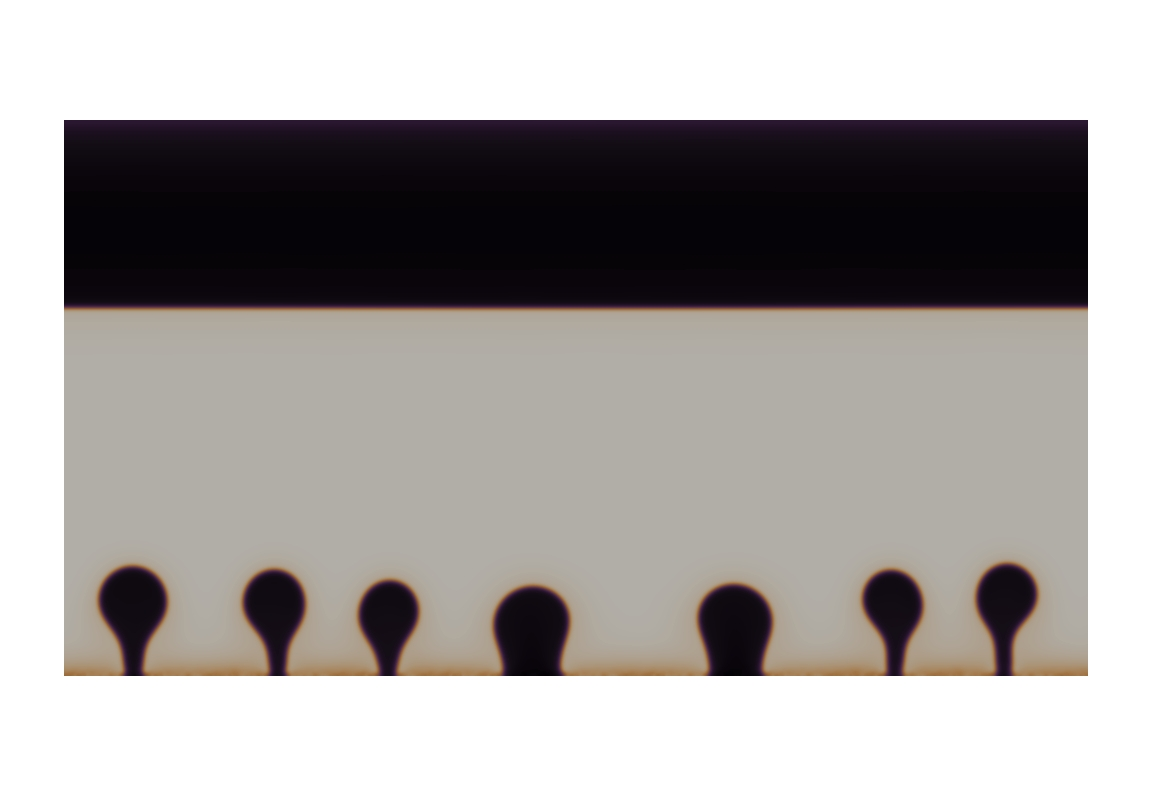
\includegraphics[width=0.8\textwidth]{Imagenes/HetBoiling/Placas6/t_34k}   
        \vspace{-10mm}
        \caption{$t^*=3.93$}     
    \end{subfigure}
    \begin{subfigure}[t]{0.9\textwidth}
        \centering
        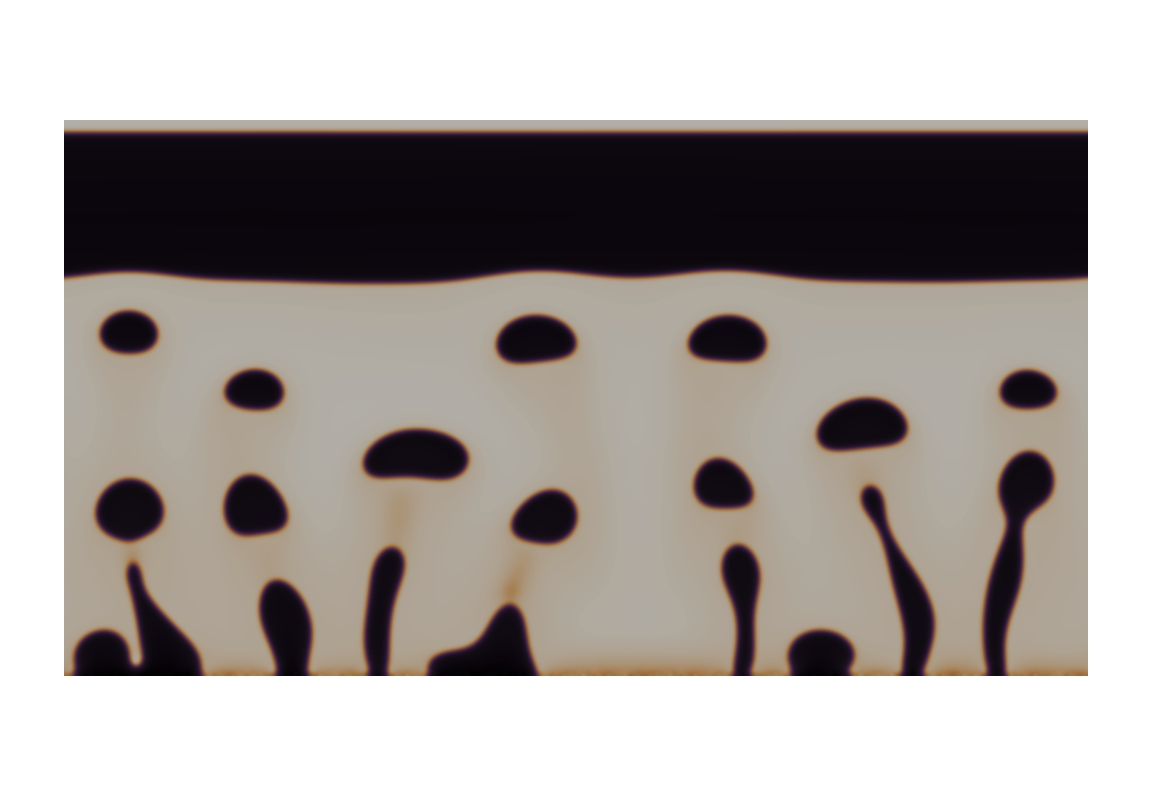
\includegraphics[width=0.8\textwidth]{Imagenes/HetBoiling/Placas6/t_80k}
        \vspace{-10mm}
        \caption{$t^*=9.24$}
    \end{subfigure}
    \begin{subfigure}[t]{0.9\textwidth}
        \centering
        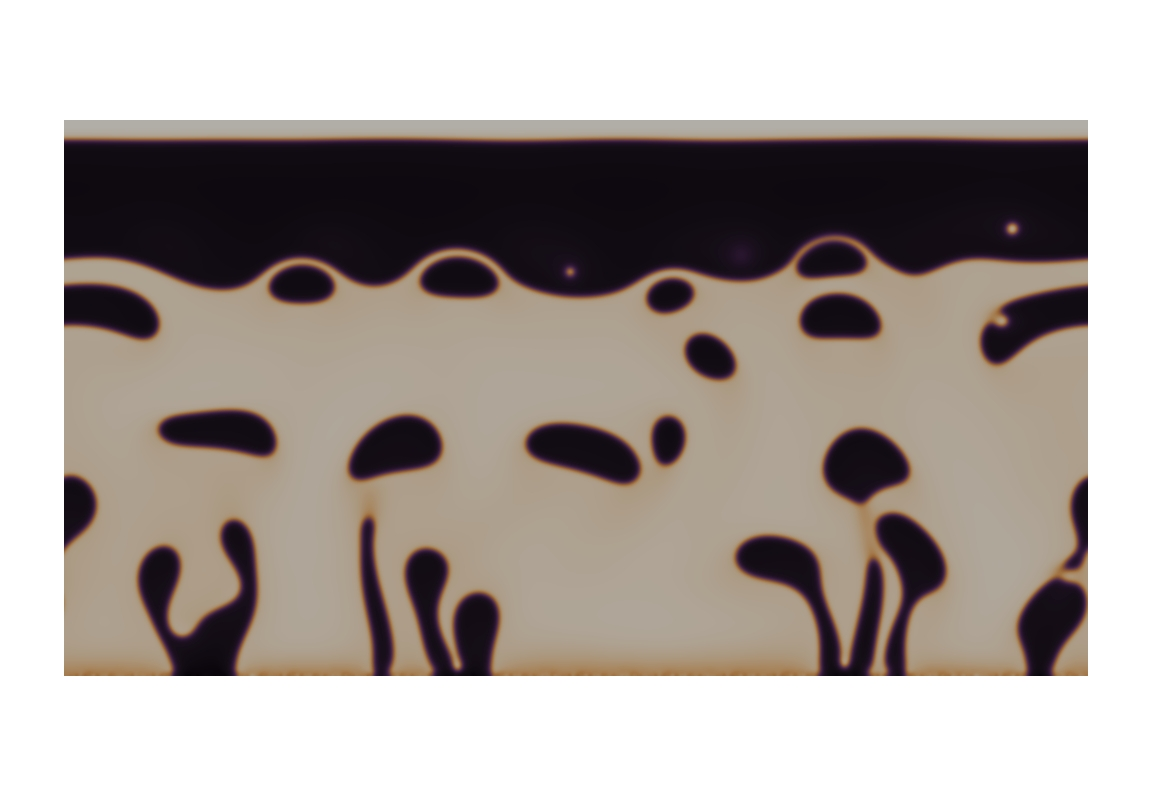
\includegraphics[width=0.8\textwidth]{Imagenes/HetBoiling/Placas6/t_120k}
        \vspace{-10mm}
        \caption{$t^*=13.86$}
    \end{subfigure}    
    \caption{Ebullici\'on sobre placas paralelas. $T_w=1.2\,T_C$.}
    \label{fig:nucleate}
\end{figure}



\begin{figure}[htb]
    \centering
    \begin{subfigure}[t]{0.9\textwidth}
        \centering
        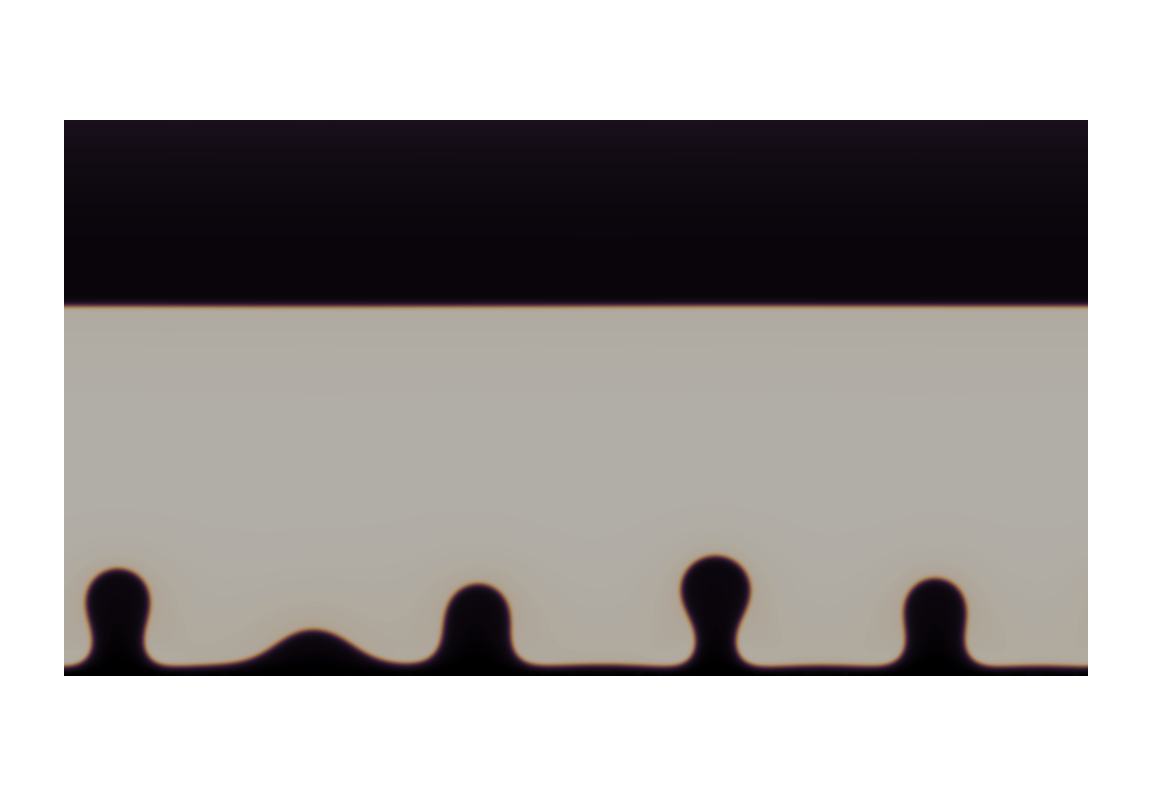
\includegraphics[width=0.8\textwidth]{Imagenes/HetBoiling/Placas7/t_140k}   
        \vspace{-10mm}
        \caption{$t^*=3.93$}     
    \end{subfigure}
    \begin{subfigure}[t]{0.9\textwidth}
        \centering
        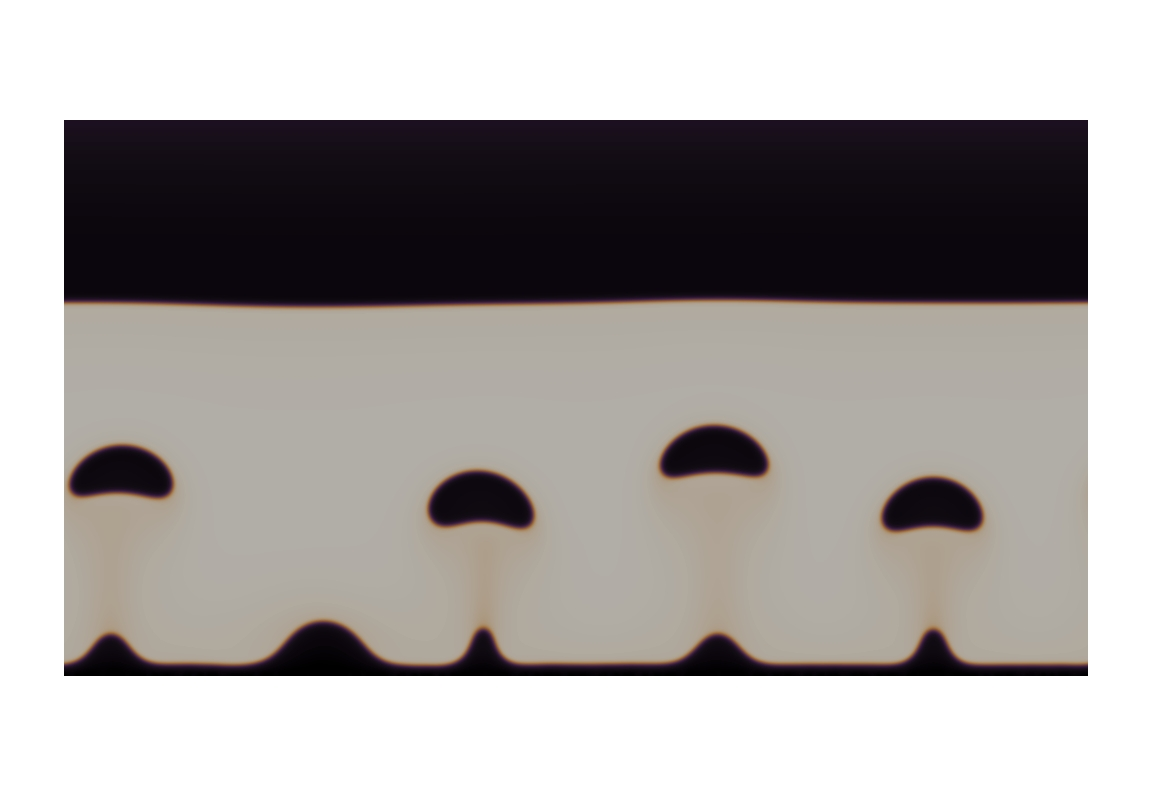
\includegraphics[width=0.8\textwidth]{Imagenes/HetBoiling/Placas7/t_160k}
        \vspace{-10mm}
        \caption{$t^*=9.24$}
    \end{subfigure}
    \begin{subfigure}[t]{0.9\textwidth}
        \centering
        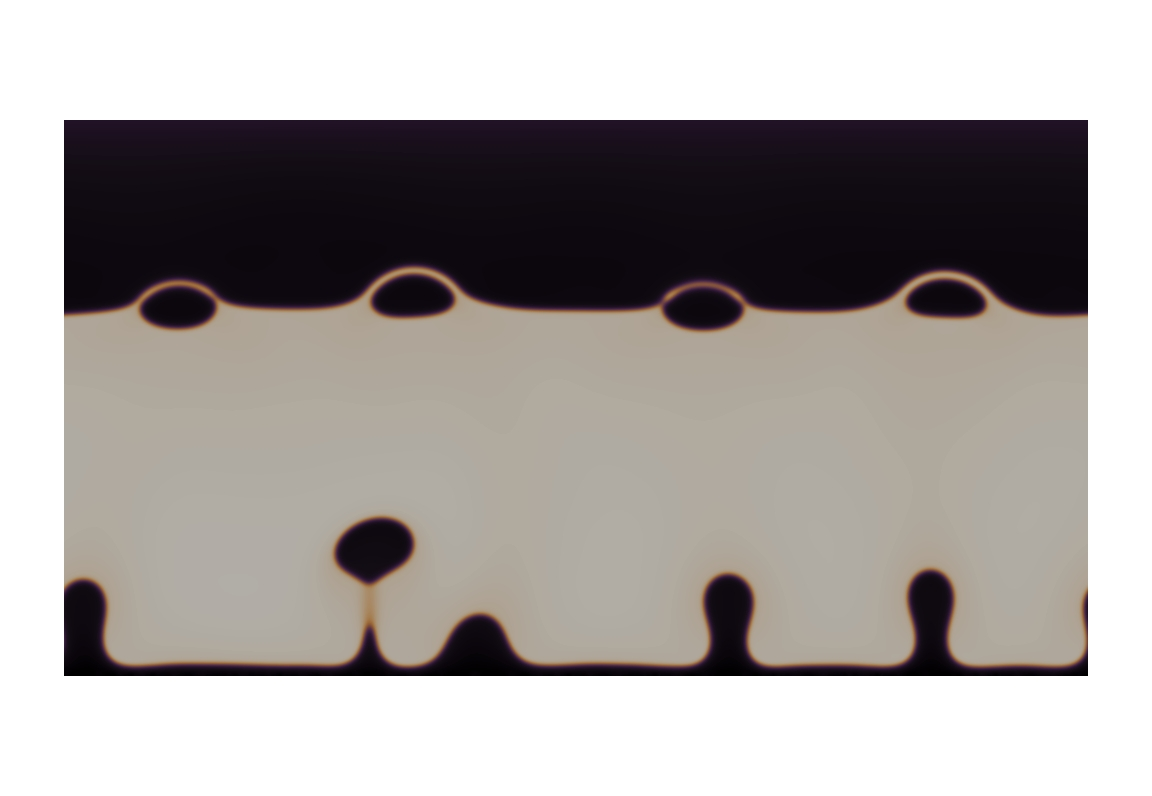
\includegraphics[width=0.8\textwidth]{Imagenes/HetBoiling/Placas7/t_200k}
        \vspace{-10mm}
        \caption{$t^*=13.86$}
    \end{subfigure}    
    \caption{Ebullici\'on sobre placas paralelas. $T_w=1.3\,T_C$.}
    \label{fig:film}
\end{figure}
\FloatBarrier




\section{Conclusiones}

En este cap\'itulo se introdujo un nuevo esquema de lattice Boltzmann en dos dimensiones, con dos funciones de distribuci\'on y operador de colisi\'on MRT, destinado a la resoluci\'on de flujos multif\'asicos con transferencia de calor. Este modelo acopla una \lbe{} de la familia \pp{} para resolver las ecuaciones hidrodin\'amicas, junto con una ecuaci\'on modificada para el transporte de energ\'ia.

A diferencia de los esquemas de LB tradicionales, la estrategia propuesta introduce una adecuada definici\'on de la distribuci\'on de equilibrio directamente en el espacio de momentos, con par\'ametros libres que pueden usarse para ajustar la difusividad t\'ermica recuperada. Adem\'as, el an\'alisis de Chapman-Enskog muestra que cuando esta distribuci\'on de equilibrio se emplea junto con una matriz de relajaci\'on con coeficientes extra-diagonales no nulos, adecuadamente definidos, la ecuaci\'on de energ\'ia macrosc\'opica se recupera sin t\'erminos adicionales hasta la escala de expansi\'on analizada. De esta forma, no es necesario aplicar correcciones expl\'icitas a los t\'erminos de fuente o a la distribuci\'on post-colisi\'on, usualmente usadas para eliminar los efectos relacionados con la simulaci\'on de ecuaciones escalares de advecci\'on-difusi\'on usando esquemas LB cl\'asicos.

El modelo propuesto es capaz de reproducir problemas num\'ericos con soluciones anal\'iticas, como distribuci\'on de temperatura y densidad en un fluido vdW estratificado, as\'i como la evoluci\'on de la interfase en un problema de Stefan unidimensional. En el primer caso, el modelo es capaz de calcular adecuadamente las distribuciones en el centro del fluido y la posici\'on de la interfase para diferentes condiciones de contorno. De forma similar a lo observado en el caso isot\'ermico, se observa consistencia del m\'etodo en unidades reducidas. En la segunda prueba, la evoluci\'on de la posici\'on de la interfase pudo ser reproducida satisfactoriamente usando diferentes combinaciones de constantes de equilibrio y par\'ametros de relajaci\'on que conducen a una misma difusividad t\'ermica, lo que evidencia el cumplimiento del comportamiento previsto por la expansi\'on de Chapman-Enskog.

Por otro lado, se analiz\'o la consistencia y orden de convergencia del modelo propuesto mediante la simulaci\'on de generaci\'on de burbujas sobre una superficie horizontal calefaccionada. Para ello, se aplic\'o una evaluaci\'on de independencia de grilla de dos pasos, tomando como base la reproducci\'on de n\'umeros adimensionales caracter\'isticos. En primer lugar, se realizaron simulaciones sobre diferentes grillas, conservando estos par\'ametros junto con el espesor de interfase adimensional. En este caso, no se observaron diferencias significativas en la evoluci\'on de la interfase entre las distintas simulaciones, lo que constituye un claro indicio de que las ecuaciones macrosc\'opicas se recuperan seg\'un lo esperado. Por otro lado, se realiz\'o un segundo conjunto de simulaciones sobre diferentes grillas, conservando los mismos n\'umeros adimensionales relevantes pero conservando el espesor de interfase en unidades de grilla. En este caso, el di\'ametro de partida adimensional converge con orden 2.18.

El problema de ebullici\'on heterog\'enea sirvi\'o adem\'as que la elecci\'on del m\'etodo usado para aplicar las condiciones de contorno influye significativamente en el proceso de crecimiento y desprendimiento de las burbujas. En particular, mientras que el modelo de Inamuro produce resultados consistentes con simulaciones efectuadas con una ecuaci\'on de energ\'ia resuelta por diferencias finitas, los m\'etodos de equilibrio y de extrapolaci\'on no conducen al rompimiento del cuello, y por lo tanto, evitan el desprendimiento de las burbujas. 

Durante el desarrollo del modelo t\'ermico se propuso una alternativa para calcular el gradiente de temperatura expl\'icitamente en el t\'ermino de fuente, que s\'olo involucra a los valores locales de la funci\'on de distribuci\'on y de la distribuci\'on de equilibrio en cada nodo. Con este esquema, no se observaron diferencias significativas con los resultados obtenidos usando diferencias finitas centradas para $\nabla T$, lo que motiva al uso de este esquema en caso de requerir una optimizaci\'on de modelos de c\'alculo paralelizados.

Finalmente, simulaciones de ebullici\'on sobre placas planas, donde se considera una condici\'on de contorno de temperatura con fluctuaciones en torno a un valor medio, muestran que el modelo permite reproducir, a nivel cuantitativo, fen\'omenos caracter\'isticos del proceso. Si bien estas simulaciones corresponden a dominios bidimensionales, y por lo tanto sin nexos directos con un caso real, se observ\'o que modificaciones en la temperatura de la superficie calefactora induce la generaci\'on de burbujas siguiendo patrones significativamente diferentes. En particular, en las condiciones de simulaci\'on presentadas se observ\'o una producci\'on de burbujas asociadas a los reg\'imenes de ebullici\'on nucleada y de ebulluci\'on de pel\'icula. 

%
%\chapter{Transferencia de calor en flujo multif\'asico tridimensional}

La metodolog\'ia propuesta en el \chap{chap:modelo2D} demostr\'o ser una alternativa robusta para simular transferencia de calor en flujo multif\'asico bidimensional. La elecci\'on de dos \red{\lbe{}} con operador de colisi\'on MRT y definidas sobre un conjunto de velocidades D2Q9 permiti\'o alcanzar una descripci\'on macrosc\'opica precisa de las ecuaciones objetivo, sin la presencia de t\'erminos no deseados en las escalas de expansi\'on analizadas. 

Este modelo bidimensional, preciso y eficiente, puede ser aplicado en problemas reales cuya descripci\'on admite una reducci\'on de dimensiones. Sin embargo, en los problemas t\'ipicos de ebullici\'on esta aproximaci\'on muchas veces no es factible, por lo que es necesario continuar con la extensi\'on del modelo de transferencia de energ\'ia a 3 dimensiones.


\section{Esquema MRT para ecuaciones hidrodin\'amicas}

Los resultados obtenidos con el modelo D2Q9 motivan el desarrollo de nuevas \lbe{} basadas en la familia \pp{}. Por lo tanto, resulta natural buscar una extensi\'on de las ecuaciones a tres dimensiones, pero que tengan como base aquellos modelos desarrollados para grillas bidimensionales.

En el caso de las ecuaciones hidrodin\'amicas, el modelo de Xu y colaboradores \cite{xu_three-dimensional_2015} constituye una extensi\'on del modelo de Li a una grilla D3Q15. Siguiendo una idea similar, este modelo introduce una \lbe{} para una funci\'on de distribuci\'on $f$ con operador de colisi\'on MRT:
\begin{equation}
	\bm{f} (\bm{x} + \bm{e}\delta_t, t+\delta_t) = \bm{M}^{-1}\left[ \bm{m} - \bm{\Lambda}(\bm{m} - \feq{m})  + \delta_t \left( \bm{I} - \dfrac{\bm{\Lambda}}{2} \bar{\bm{S}} \right) + \bm{C}\right],
	\label{eq:lbe_xu}	
\end{equation}
con
\begin{subequations}
	\begin{equation}
		\rho = \sum_{\alpha} f_{\alpha},
	\end{equation}
	\begin{equation}
		\rho \bm{u} = \sum_{\alpha} f_{\alpha} \bm{e}_{\alpha} + \dfrac{\delta_t}{2}\bm{F},
	\end{equation}
\end{subequations}
donde $\bm{F} = \bm{F}_b + \bm{F}_i$ es la fuerza total sobre los nodos, es decir, la combinaci\'on de fuerza boyante y de interaci\'on. Usando la notaci\'on usual, $\bm{m} = \bm{Mf}$ y $\feq{m} = \bm{M}\feq{f}$ corresponden a la proyecci\'on de $\bm{f}$ y $\feq{f}$ en el espacio de momentos respectivamente, de modo que la distribuci\'on de equilibrio en el espacio de momentos resulta:
\begin{equation}
	\begin{split}
		\feq{m} = \rho \left( 1, -1+|\bm{u}|^2, 1-5|\bm{u}|^2, u_x, -\dfrac{7}{3}u_x, u_y, -\dfrac{7}{3}u_y, u_z, -\dfrac{7}{3}u_z, 2u_x^2-u_y^2-u_z^2, \right.\\
		\left.\phantom{\dfrac{1}{1}} u_y^2 - u_z^2, u_xu_y, u_yu_z,u_xu_z,0 \right)^T	.
	\end{split}	
\end{equation}

Por otro lado, la matriz de colisi\'on $\bm{\Lambda}$ corresponde a una matriz diagonal con coeficientes definidos como:
\begin{equation}
	\bm{\Lambda} = \mbox{diag}(\tau_{\rho}^{-1}, \tau_{e}^{-1}, \tau_{\varepsilon}^{-1}, \tau_{j}^{-1}, \tau_{q}^{-1}, \tau_{j}^{-1}, \tau_{q}^{-1}, \tau_{j}^{-1}, \tau_{q}^{-1}, \tau_{\nu}^{-1}, \tau_{\nu}^{-1}, \tau_{\nu}^{-1}, \tau_{\nu}^{-1}, \tau_{\nu}^{-1}, \tau_{xyz}^{-1}),
\end{equation}
mientras que el t\'ermino de fuerza $\bm{S}$ se define en el espacio de momentos mediante:
\begin{equation}
 \bar{\bm{S}} = 
 \left[ 
 	\begin{array}{c} 
 		0	\\
 		2 \bm{u} \cdot \bm{F} + \dfrac{6\sigma |\bm{F}|^2}{\psi^2 \delta_t (\tau_e-0.5)} \\
 		-10 \bm{u} \cdot \bm{F} \\
 		F_x \\
 		-\dfrac{7}{3}F_x \\
 		F_y \\
 		-\dfrac{7}{3}F_y \\
 		F_z \\
 		-\dfrac{7}{3}F_z \\ 		
		4u_xF_x - 2u_yF_y - 2u_zF_z \\
		2u_yF_y - 2u_zF_z \\
		u_xF_y + u_yF_x \\
		u_yF_z + u_zF_y \\
		u_xF_z + u_zF_x \\
		0
 	\end{array} 
 \right]
 \label{eq:s_xu}
\end{equation}

De manera similar a lo que ocurre con la versi\'on de Li \cite{li_lattice_2013}, el par\'ametro $\sigma$ se utiliza para ajustar parcialmente el problema de inconsistencia termodin\'amica, es decir, corregir las densidades de coexistencia recuperadas para cada fase. 

La \eq{eq:lbe_xu} incorpora un t\'ermino adicional $\bm{C}$:
\begin{equation}
 \bm{C} = 
 \left[ 
 	\begin{array}{c} 
 		0	\\
 		\dfrac{4}{5} \tau_{e}^{-1}(R_{xx} + R_{yy} + R_{zz}) \\
 		0 \\
 		0 \\
 		0 \\
 		0 \\
 		0 \\
 		0 \\
 		0 \\ 		
		-\tau_{\nu}^{-1}(2R_{xx} - R_{yy} - R_{zz}) \\
		-\tau_{\nu}^{-1}(R_{yy} - R_{zz}) \\
		-\tau_{\nu}^{-1}R_{xy} \\
		-\tau_{\nu}^{-1}R_{yz} \\
		-\tau_{\nu}^{-1}R_{xz} \\
		0
 	\end{array} 
 \right],
 \label{eq:c_xu}
\end{equation}
donde las componentes $R_{\beta\gamma}$ corresponden al tensor $\bm{R}$ definido como:
\begin{equation}
 \bm{R} = \kappa \dfrac{G}{2} \psi(\bm{x}) \sum_{\alpha} w(|\bm{e}_{\alpha}|^2) \left[ \psi(\bm{x}+\bm{e}_{\alpha}) - \psi(\bm{x}) \right] \bm{e}_{\alpha}\bm{e}_{\alpha}.
	\label{eq:R_xu}
\end{equation}

En este caso, puede demostrarse que la incorporaci\'on del t\'ermino $\bm{C}$ permite  ajustar la tensi\'on superficial recuperada mediante la constante $\kappa$ de la \eq{eq:R_xu}.

\red{Revisar la unificaci\'on de las constantes w}

El an\'alisis de Chapman-Enskog de este esquema muestra que es posible recuperar las siguientes ecuaci\'ones de conservaci\'on de masa e impulso lineal:
\begin{subequations}
	\begin{equation}
		\dfrac{\partial \rho}{\partial t} + \nabla \cdot (\rho \bm{u}) = 0,
	\end{equation}
	\begin{equation}
		\begin{aligned}
		\dfrac{\partial(\rho\bm{u})}{\partial t} + \nabla \cdot (\rho \bm{u} \bm{u})  = &-\nabla \cdot(\rho c_s^2)\bm{I} + \nabla \cdot \bm{\Pi} + \bm{F} - 2G^2 c^4 \sigma \nabla \cdot (|\nabla \psi|^2 \bm{I}) \\
		& -\nabla \cdot \left[ \kappa \dfrac{Gc^4}{6} (\psi \nabla^2 \psi \bm{I} - \psi \nabla \nabla \psi) \right],
		\end{aligned}
	\end{equation}
	\label{eq:xu_macro}
\end{subequations}
donde el tensor de tensiones $\bm{\Pi}$ se define como:
\begin{equation}
	\bm{\Pi} = \rho \nu \left[ \nabla \bm{u} + (\nabla \bm{u})^T \right] + \rho \left( \xi - \dfrac{2}{3}\nu \right) (\nabla \cdot \bm{u})\bm{I},
\end{equation}
y las viscosidades cinem\'atica y \red{de bulk} corresponden a:
\begin{subequations}
	\begin{equation}
		\nu = \dfrac{1}{3} \left( \tau_{\nu} - \dfrac{1}{2}\right) \delta_t,
	\end{equation}
	\begin{equation}
		\xi = \dfrac{2}{9} \left( \tau_{e} - \dfrac{1}{2}\right) \delta_t.
	\end{equation}	
\end{subequations}

Como puede observarse, la \eq{eq:xu_macro} es similar al conjunto de ecuaciones recuperadas por el modelo bidimensional de Li (\eq{eq:li_macro}), salvo por la presencia de t\'erminos dependientes de $\kappa$ que contribuyen a la recuperaci\'on de tensi\'on superficial en la interfase. En particular, si se utiliza le expresi\'on discreta para el tensor de presiones introducida por Shan \cite{shan_pressure_2008}, es posible ver que la forma macorsc\'opica de este tensor finalmente resulta:
\begin{equation}
	\bm{P} = \left[ \rho c_s^2 + \dfrac{G c^2}{2} \psi^2 + \dfrac{G c^4}{12} (1+2\kappa) \psi \nabla^2 \psi + 2 \sigma G^2 c^4 |\nabla \psi|^2\right] \bm{I} + \dfrac{G c^4}{6} (1-\kappa) \psi \nabla \nabla \psi.
\end{equation}


\subsection{Condiciones de contorno}




\section{Esquema MRT para ecuaci\'on de energ\'ia}

En el \chap{chap:modelo2D} se mostr\'o que es posible acoplar una segunda \lbe{} a un esquema de la famila \pp{}, y de esta forma poder simular transferencia de calor y cambio de fase en flujos multif\'asicos. En particular, si se elige adecuadamente a la distribuci\'on de equilibrio, matriz de relajaci\'on y t\'ermino fuente, se mostr\'o formalmente que es posible recuperar una soluci\'on macrosc\'opica dada por la \eq{eq:markus}, sin t\'erminos adicionales hasta la escala de expansi\'on analizada. Por otro lado, la metodolog\'ia empleada demostr\'o proveer un camino consistente para el desarrollo de nuevas \lbe{} para la resoluci\'on de ecuaciones de energ\'ia similares, eficientes y flexibles en la reproducci\'on de las propiedades macrosc\'opicas relevantes.

Estas caracter\'isticas positivas observadas en el modelo bidimensional motivan la continuaci\'on de esta l\'inea de desarrollo. De esta manera, la nueva propuesta consiste en emplear una \lbe{} con operador de colisi\'on MRT sobre un conjunto de velocidades D3Q15:
\begin{subequations}
	\begin{equation}
		\bm{g}(\bm{x} + \bm{e} \delta_t, t+\delta_t) = \bm{M}^{-1} \left[ \bm{n} - \bm{Q}(\bm{n} - \feq{n}) + \delta_t \left( \bm{I}-\dfrac{\bm{Q}}{2}\right) \bm{\Gamma}\right],
		\label{eq:g_model_3d}
	\end{equation}	
	\begin{equation}
		T = \sum_{\alpha} g_{\alpha} + \dfrac{\delta_t}{2} \Gamma_0,
	\end{equation}
\end{subequations}
donde las variables del miembro derecho se encuentran definidas en $(\bm{x},t)$. En este caso, $\bm{n} = \bm{Mg}$,  $\feq{n} = \bm{M}\feq{g}$, y $\bm{\Gamma}$ corresponde a un t\'ermino de fuente definido en el espacio de momentos. 

Continuando con las ideas desarrolladas en el \chap{chap:modelo2D}, es posible introducir una distribuci\'on de equilibrio y el t\'ermino de fuente directamente en el espacio de momentos:
\begin{equation}
	\feq{n} = T ( 1, \alpha_1, \alpha_2, \alpha_3u_x, \alpha_4u_x, \alpha_5u_y, \alpha_6u_y, \alpha_7u_z, \alpha_8u_z,0,0,0,0,0,0)^T,
\end{equation}
\begin{equation}
	\bm{\Gamma} = (s,0,0,0,0,0,0,0,0,0,0,0,0,0,0)^T.	
\end{equation}

Por otro lado, es necesario incluir una matriz de relajaci\'on con coeficientes no nulos en la diagonal, que en este caso corresponde a los elementos $q_{34}$, $q_{56}$ y $q_{78}$.
%\setcounter{MaxMatrixCols}{15}
%\begin{equation}
%	\bm{Q}=
%	\begin{bmatrix}
%	q_0 & 0 & 0 & 0 & 0 & 0 & 0 & 0 & 0 & 0 & 0 & 0 & 0 & 0 & 0 \\
%	0 & q_1 & 0 & 0 & 0 & 0 & 0 & 0 & 0 & 0 & 0 & 0 & 0 & 0 & 0 \\
%	0 & 0 & q_2 & 0 & 0 & 0 & 0 & 0 & 0 & 0 & 0 & 0 & 0 & 0 & 0 \\
%	0 & 0 & 0 & q_3 & q_{34} & 0 & 0 & 0 & 0 & 0 & 0 & 0 & 0 & 0 & 0 \\
%	0 & 0 & 0 & 0 & q_4 & 0 & 0 & 0 & 0 & 0 & 0 & 0 & 0 & 0 & 0 \\
%	0 & 0 & 0 & 0 & 0 & q_5 & q_{56} & 0 & 0 & 0 & 0 & 0 & 0 & 0 & 0 \\
%	0 & 0 & 0 & 0 & 0 & 0 & q_6 & 0 & 0 & 0 & 0 & 0 & 0 & 0 & 0 \\
%	0 & 0 & 0 & 0 & 0 & 0 & 0 & q_7 & q_{78} & 0 & 0 & 0 & 0 & 0 & 0 \\
%	0 & 0 & 0 & 0 & 0 & 0 & 0 & 0 & q_8 & 0 & 0 & 0 & 0 & 0 & 0 \\
%	0 & 0 & 0 & 0 & 0 & 0 & 0 & 0 & 0 & q_{9} & 0 & 0 & 0 & 0 & 0 \\
%	0 & 0 & 0 & 0 & 0 & 0 & 0 & 0 & 0 & 0 & q_{10} & 0 & 0 & 0 & 0 \\
%	0 & 0 & 0 & 0 & 0 & 0 & 0 & 0 & 0 & 0 & 0 & q_{11} & 0 & 0 & 0 \\
%	0 & 0 & 0 & 0 & 0 & 0 & 0 & 0 & 0 & 0 & 0 & 0 & q_{12} & 0 & 0 \\
%	0 & 0 & 0 & 0 & 0 & 0 & 0 & 0 & 0 & 0 & 0 & 0 & 0 & q_{13} & 0 \\
%	0 & 0 & 0 & 0 & 0 & 0 & 0 & 0 & 0 & 0 & 0 & 0 & 0 & 0 & q_{14}
%	\end{bmatrix}
%\end{equation}

La expansi\'on en serie de Taylor de la \eq{eq:g_model_3d} lleva a una expresi\'on similar a la \eq{eq:model_2d_momento}:
\begin{equation}
	\dcm \bm{n} + \dfrac{\delta_t}{2} \dcm^2 \bm{n} = -\dfrac{1}{\delta_t}\bm{Q}(\bm{n} - \feq{n}) + \delta_t \left( \bm{I}-\dfrac{\bm{Q}}{2}\right) \bm{\Gamma},
	\label{eq:model_3d_momento}
\end{equation}
y, por lo tanto, a la misma descomposici\'on en escalas de $\varepsilon$ dentro del an\'alisis de Chapman-Enskog. En particular, si se aplica la expansi\'on dada por>
\begin{subequations}
	\begin{equation}
		\bm{n} = \bc{n}{0} + \varepsilon \bc{n}{1} + \varepsilon^2 \bc{n}{2} + \cdots = \sum_{k=0}^{\infty} \varepsilon^k \bc{n}{k}
	\end{equation}
	\begin{equation}
		\dfrac{\partial}{\partial t} = \varepsilon \dfrac{\partial}{\partial t_1} + 	\varepsilon^2 \dfrac{\partial}{\partial t_2}
	\end{equation}
	\begin{equation}
		\dfrac{\partial}{\partial x_{\beta}} = \varepsilon \dfrac{\partial}{\partial x_{\beta_1}}
	\end{equation}
	\begin{equation}
		\bm{\Gamma} = \varepsilon \bc{\Gamma}{1},
	\end{equation}
\end{subequations}
entonces puede descomponerse a la \eq{eq:model_3d_momento} en ecuaciones individuales para cada potencia de $\varepsilon$:
\begin{subequations}
	\begin{align}
		\varepsilon^0: && \bc{n}{0} = \feq{n} \label{eq:eps_0_3d}\\
		\varepsilon^1: && \dcmuno \bc{n}{0} - \bc{\Gamma}{1} = -\dfrac{1}{\delta_t} \bm{Q} \left( \bc{n}{1} + \dfrac{\delta_t}{2} \bc{\Gamma}{1} \right)  \label{eq:eps_1_3d}\\
		\varepsilon^2: && \dcmuno \left( \bm{I}-\dfrac{\bm{Q}}{2}\right) \left( \bc{n}{1} + \dfrac{\delta_t}{2} \bc{\Gamma}{1} \right) + \dfrac{\partial \bc{n}{0}}{\partial t_2}  =  -\dfrac{1}{\delta_t} \bm{Q} \bc{n}{2}. \label{eq:eps_2_3d}
	\end{align}
\end{subequations}

La definici\'on de las matrices $\hat{\bm{E}}_{\beta}$ es similar a la del caso bidimensional, por lo que corresponden a $\hat{\bm{E}}_{\beta} = \bm{M} \bm{E}_{\beta} \bm{M}^{-1}$, con $\bm{E}_{\beta} = diag(e_{0\beta} \cdots e_{q-1\beta})$. En una grilla D3Q15, donde $\beta=x,y,z$ y se tiene un conjunto diferente de velocidades de grilla, estas matrices resultan:
\setcounter{MaxMatrixCols}{15}
\begin{equation}
	\hat{\bm{E}}_{x}=
	\begin{bmatrix}
	0 & 0 & 0 & 1 & 0 & 0 & 0 & 0 & 0 & 0 & 0 & 0 & 0 & 0 & 0 \\
	0 & 0 & 0 & 3/5 & 2/5 & 0 & 0 & 0 & 0 & 0 & 0 & 0 & 0 & 0 & 0 \\
	0 & 0 & 0 & 0 & 1 & 0 & 0 & 0 & 0 & 0 & 0 & 0 & 0 & 0 & 0 \\
	2/3 & 1/3 & 0 & 0 & 0 & 0 & 0 & 0 & 0 & 1/3 & 0 & 0 & 0 & 0 & 0 \\
	0 & 8/9 & 1/9 & 0 & 0 & 0 & 0 & 0 & 0 & -4/3 & 0 & 0 & 0 & 0 & 0 \\
	0 & 0 & 0 & 0 & 0 & 0 & 0 & 0 & 0 & 0 & 0 & 1 & 0 & 0 & 0 \\
	0 & 0 & 0 & 0 & 0 & 0 & 0 & 0 & 0 & 0 & 0 & 1 & 0 & 0 & 0 \\
	0 & 0 & 0 & 0 & 0 & 0 & 0 & 0 & 0 & 0 & 0 & 0 & 0 & 1 & 0 \\
	0 & 0 & 0 & 0 & 0 & 0 & 0 & 0 & 0 & 0 & 0 & 0 & 0 & 1 & 0 \\
	0 & 0 & 0 & 2/5 & -2/5 & 0 & 0 & 0 & 0 & 0 & 0 & 0 & 0 & 0 & 0 \\
	0 & 0 & 0 & 0 & 0 & 0 & 0 & 0 & 0 & 0 & 0 & 0 & 0 & 0 & 0 \\
	0 & 0 & 0 & 0 & 0 & 4/5 & 1/5 & 0 & 0 & 0 & 0 & 0 & 0 & 0 & 0 \\
	0 & 0 & 0 & 0 & 0 & 0 & 0 & 0 & 0 & 0 & 0 & 0 & 0 & 0 & 1 \\
	0 & 0 & 0 & 0 & 0 & 0 & 0 & 4/5 & 1/5 & 0 & 0 & 0 & 0 & 0 & 0 \\
	0 & 0 & 0 & 0 & 0 & 0 & 0 & 0 & 0 & 0 & 0 & 0 & 1 & 0 & 0 \\
	\end{bmatrix},
\end{equation} 

\begin{equation}
	\hat{\bm{E}}_{y}=
	\begin{bmatrix}
	0 & 0 & 0 & 0 & 1 & 0 & 0 & 0 & 0 & 0 & 0 & 0 & 0 & 0 & 0 \\
	0 & 0 & 0 & 0 & 3/5 & 2/5 & 0 & 0 & 0 & 0 & 0 & 0 & 0 & 0 & 0 \\
	0 & 0 & 0 & 0 & 0 & 0 & 1 & 0 & 0 & 0 & 0 & 0 & 0 & 0 & 0 \\
	0 & 0 & 0 & 0 & 0 & 0 & 0 & 0 & 0 & 0 & 0 & 1 & 0 & 0 & 0 \\
	0 & 0 & 0 & 0 & 0 & 0 & 0 & 0 & 0 & 0 & 0 & 1 & 0 & 0 & 0 \\
	2/3 & 1/3 & 0 & 0 & 0 & 0 & 0 & 0 & 0 & -1/6 & 1/2 & 0 & 0 & 0 & 0 \\
	0 & 8/9 & 1/9 & 0 & 0 & 0 & 0 & 0 & 0 & 2/3 & -2 & 0 & 0 & 0 & 0 \\
	0 & 0 & 0 & 0 & 0 & 0 & 0 & 0 & 0 & 0 & 0 & 0 & 0 & 1 & 0 \\
	0 & 0 & 0 & 0 & 0 & 0 & 0 & 0 & 0 & 0 & 0 & 0 & 0 & 1 & 0 \\
	0 & 0 & 0 & 0 & -1/5 & 1/5 & 0 & 0 & 0 & 0 & 0 & 0 & 0 & 0 & 0 \\
	0 & 0 & 0 & 0 & 1/5 & -1/5 & 0 & 0 & 0 & 0 & 0 & 0 & 0 & 0 & 0 \\
	0 & 0 & 0 & 4/5 & 1/5 & 0 & 0 & 0 & 0 & 0 & 0 & 0 & 0 & 0 & 0 \\
	0 & 0 & 0 & 0 & 0 & 0 & 0 & 4/5 & 1/5 & 0 & 0 & 0 & 0 & 0 & 0 \\
	0 & 0 & 0 & 0 & 0 & 0 & 0 & 0 & 0 & 0 & 0 & 0 & 0 & 0 & 1 \\
	0 & 0 & 0 & 0 & 0 & 0 & 0 & 0 & 0 & 0 & 0 & 0 & 0 & 1 & 0 \\
	\end{bmatrix}
\end{equation} 

y 

\begin{equation}
	\hat{\bm{E}}_{z}=
	\begin{bmatrix}
	0 & 0 & 0 & 0 & 0 & 0 & 0 & 1 & 0 & 0 & 0 & 0 & 0 & 0 & 0 \\
	0 & 0 & 0 & 0 & 0 & 0 & 0 & 3/5 & 2/5 & 0 & 0 & 0 & 0 & 0 & 0 \\
	0 & 0 & 0 & 0 & 0 & 0 & 0 & 0 & 1 & 0 & 0 & 0 & 0 & 0 & 0 \\
	0 & 0 & 0 & 0 & 0 & 0 & 0 & 0 & 0 & 0 & 0 & 0 & 0 & 1 & 0 \\
	0 & 0 & 0 & 0 & 0 & 0 & 0 & 0 & 0 & 0 & 0 & 0 & 0 & 1 & 0 \\
	0 & 0 & 0 & 0 & 0 & 0 & 0 & 0 & 0 & 0 & 0 & 0 & 1 & 0 & 0 \\
	0 & 0 & 0 & 0 & 0 & 0 & 0 & 0 & 0 & 0 & 0 & 0 & 1 & 0 & 0 \\
	2/3 & 1/3 & 0 & 0 & 0 & 0 & 0 & 0 & 0 & -1/6 & -1/2 & 0 & 0 & 0 & 0 \\
	0 & 8/9 & 1/9 & 0 & 0 & 0 & 0 & 0 & 0 & 2/3 & 2 & 0 & 0 & 0 & 0 \\
	0 & 0 & 0 & 0 & 0 & 0 & 0 & -1/5 & 1/5 & 0 & 0 & 0 & 0 & 0 & 0 \\
	0 & 0 & 0 & 0 & 0 & 0 & 0 & -1/5 & 1/5 & 0 & 0 & 0 & 0 & 0 & 0 \\
	0 & 0 & 0 & 0 & 0 & 0 & 0 & 0 & 0 & 0 & 0 & 0 & 0 & 0 & 1 \\
	0 & 0 & 0 & 0 & 0 & 4/5 & 1/5 & 0 & 0 & 0 & 0 & 0 & 0 & 0 & 0 \\
	0 & 0 & 0 & 4/5 & 1/5 & 0 & 0 & 0 & 0 & 0 & 0 & 0 & 0 & 0 & 0 \\
	0 & 0 & 0 & 0 & 0 & 0 & 0 & 0 & 0 & 0 & 0 & 1 & 0 & 0 & 0 \\
	\end{bmatrix}.
\end{equation} 

En definitiva, el desarrollo de Taylor y la expansi\'on de Chapman-Enskog empleada en el \chap{chap:modelo2D} son aplicables al nuevo conjunto de velocidades, aunque naturalmente deben considerarse nuevas estructuras para $\feq{n}$, $\bm{Q}$ y $\hat{\bm{E}}_{\beta}$. 

La ecuaci\'on recuperada en la escala $\varepsilon^1$ puede obtenerse a partir de la primera componenete de la \eq{eq:eps_1_3d}:
\begin{equation}
	\dfrac{\partial \nce{0}{0}}{\partial t_1} 
	+ \dfrac{\partial \nce{3}{0}}{\partial x_1}
	+ \dfrac{\partial \nce{5}{0}}{\partial y_1}
	+ \dfrac{\partial \nce{7}{0}}{\partial z_1}		
	- \Gamma_0^{(1)}
	= - \dfrac{1}{\delta_t} q_0 \left( \nce{0}{1} + \dfrac{\delta_t}{2} \Gamma_0^{(1)} \right).
	\label{eq:eps1_comp_3d}
\end{equation}

Usando la descomposici\'on de escalas de la \eq{eq:ncero_che}, es decir:
\begin{equation}
	\begin{aligned}
		\varepsilon^0: && \nce{0}{0} = n_0^{eq} \\
		\varepsilon^1: && \nce{0}{1} + \dfrac{\delta_t}{2} \Gamma_0^{(1)} = 0\\
		\varepsilon^2: && \nce{0}{2} = 0 \\
		&\vdots& \\
		\varepsilon^k: && \nce{0}{k} = 0 \quad \forall \, k > 2,
	\end{aligned}
\end{equation}
entonces puede reescribirse a la \eq{eq:eps1_comp_3d} como:
\begin{equation}
	\dfrac{\partial T}{\partial t_1} 
	+ \dfrac{\partial (\alpha_3 T u_x)}{\partial x_1}
	+ \dfrac{\partial (\alpha_5 T u_y)}{\partial y_1}
	+ \dfrac{\partial (\alpha_7 T u_z)}{\partial z_1}		
	- \Gamma_0^{(1)} = 0
\end{equation}

Por lo tanto, si $\alpha_3 = \alpha_5 = \alpha_7 = 1$, se obtiene una ecuaci\'on recuperada en la escala $\varepsilon^1$:
\begin{equation}
	\dfrac{\partial T}{\partial t_1}  + \nabla_1 \cdot (T \bm{u}) - \Gamma_0^{(1)} = 0
	\label{eq:eps1_T_3d}
\end{equation}

Por otro lado, la ecuaci\'on recuperada en la escala $\varepsilon^2$ puede obtenerse a partir de la primera componente de la \eq{eq:eps_2_3d}:
\begin{equation}
	\dfrac{\partial \nce{0}{0}}{\partial t_2} 
	+ \dfrac{\partial \nces{0}{1}}{\partial t_1} 	
	+ \dfrac{\partial \nces{3}{0}}{\partial x_1}
	+ \dfrac{\partial \nces{5}{0}}{\partial y_1}
	+ \dfrac{\partial \nces{7}{0}}{\partial z_1}		
	= - \dfrac{1}{\delta_t} q_0 \nce{0}{2} = 0,
	\label{eq:eps2_comp_3d}
\end{equation}
donde
\begin{subequations}
	\begin{equation}
		\nces{0}{1} = \left( 1 - \dfrac{q_0}{2} \right) \left( \nce{0}{1} + \dfrac{\delta_t}{2} \Gamma_0^{(1)} \right) = 0,
	\end{equation}
	\begin{equation}
		\nces{3}{1} = \left( 1 - \dfrac{q_3}{2} \right) \nce{3}{1} + \dfrac{q_{34}}{2}\nce{4}{1},
		\label{eq:n3star_3d}
	\end{equation}	
	\begin{equation}
		\nces{5}{1} = \left( 1 - \dfrac{q_5}{2} \right) \nce{5}{1} + \dfrac{q_{56}}{2}\nce{6}{1},
	\end{equation}		
	\begin{equation}
		\nces{7}{1} = \left( 1 - \dfrac{q_7}{2} \right) \nce{7}{1} + \dfrac{q_{78}}{2}\nce{8}{1}.
	\end{equation}			
\end{subequations}

De esta manera, se necesitan ecuaciones que permitan expresar a $\nce{3}{1}$, $\nce{4}{1}$, $\nce{5}{1}$, $\nce{6}{1}$, $\nce{7}{1}$ y $\nce{8}{1}$ en funci\'on de las variables macrosc\'opicas, es decir $\rho$, $\bm{u}$ y $T$. Nuevamente, esta descripci\'on puede obtenerse a partir de las componentes relevantes de la \eq{eq:eps_1_3d}, como se ejemplifica para $\nce{3}{1}$:
\begin{equation}
	\dfrac{\partial \nce{3}{0}}{\partial t_1} 
	+ \dfrac{2}{3} \dfrac{\partial \nce{0}{0}}{\partial x_1}
	+ \dfrac{1}{3} \dfrac{\partial \nce{1}{0}}{\partial x_1}	
	+ \dfrac{1}{3} \dfrac{\partial \nce{9}{0}}{\partial x_1}	
	+ \dfrac{\partial \nce{11}{0}}{\partial y_1}	
	+ \dfrac{\partial \nce{13}{0}}{\partial z_1}	
	= -\dfrac{1}{\delta_t} q_3 \nce{3}{1} -\dfrac{1}{\delta_t} q_{34} \nce{4}{1}
\end{equation}
\begin{equation}
	\dfrac{\partial (Tu_x)}{\partial t_1} 
	+ \dfrac{\partial}{\partial x_1} \left( \dfrac{2+\alpha_1}{3}T \right)
	= -\dfrac{1}{\delta_t} q_3 \nce{3}{1} -\dfrac{1}{\delta_t} q_{34} \nce{4}{1}
	\label{eq:n3_eps1_3d}
\end{equation}

Por otro lado, para $\nce{4}{1}$ se tiene:
\begin{equation}
	\dfrac{\partial \nce{4}{0}}{\partial t_1} 
	+ \dfrac{8}{9} \dfrac{\partial \nce{1}{0}}{\partial x_1}
	+ \dfrac{1}{9} \dfrac{\partial \nce{2}{0}}{\partial x_1}	
	- \dfrac{4}{3} \dfrac{\partial \nce{9}{0}}{\partial x_1}	
	+ \dfrac{\partial \nce{11}{0}}{\partial y_1}	
	+ \dfrac{\partial \nce{13}{0}}{\partial z_1}	
	= -\dfrac{1}{\delta_t} q_4 \nce{4}{1},
\end{equation}
y si $\alpha_4=-1$ resulta:
\begin{equation}
	-\dfrac{\partial (Tu_x)}{\partial t_1} 
	+ \dfrac{\partial}{\partial x_1} \left( \dfrac{8\alpha_1+\alpha_2}{9}T \right)
	=-\dfrac{1}{\delta_t} q_4 \nce{4}{1}
	\label{eq:n4_eps1_3d}
\end{equation}

Si se despejan $\nce{3}{1}$ y $\nce{4}{1}$ de las \eqs{eq:n3_eps1_3d}{eq:n4_eps1_3d}, entonces puede reescribirse a la \eq{eq:n3star_3d} como:
\begin{equation}
	\begin{aligned}
	    \nces{3}{1} = &- \delta_t \left( \dfrac{1}{q_3} - \dfrac{1}{2} \right) \left[ \dfrac{\partial (Tu_x)}{\partial t_1} + \dfrac{\partial}{\partial x_1} \left( \dfrac{2+\alpha_1}{3}T \right) \right] \\
	    &+ \delta_t \dfrac{q_{34}}{q_3 q_4} \left[ -\dfrac{\partial (Tu_x)}{\partial t_1} + \dfrac{\partial}{\partial x_1} \left( \dfrac{8\alpha_1+\alpha_2}{9}T \right) \right]
	\end{aligned}
	\label{eq:n3star_final_3d}
\end{equation}

Por lo tanto, es posible ver que si el coeficiente de relajaci\'on $q_{34}$ satisface
\begin{equation}
	q_{34} = q_4 \left( \dfrac{q_3}{2} - 1 \right),
\end{equation}
entonces se anulan las derivadas temporales de $\nces{3}{1}$ y la \eq{eq:n3star_final_3d} finalmente resulta:
\begin{equation}
	\nces{3}{1} = -\delta_t \left( \dfrac{1}{q_3} - \dfrac{1}{2} \right) \dfrac{\partial}{\partial x_1} \left( \dfrac{6 + 11\alpha_1+\alpha_2}{9}T \right).
	\label{eq:n3star_macro 3d}
\end{equation}

Este mismo procedimiento puede utilizarse para reescribir a $\nces{5}{1}$ y $\nces{7}{1}$. En particular, si $\alpha_6 = \alpha_8 = -1$, y definiendo los coeficientes de relajaci\'on $q_{56}$ y $q_{78}$ como:
\begin{equation}
	q_{56} = q_6 \left( \dfrac{q_{5}}{2} - 1 \right),
\end{equation}
\begin{equation}
	q_{78} = q_8 \left( \dfrac{q_{7}}{2} - 1 \right),
\end{equation}
entonces se tiene:
\begin{equation}
	\nces{5}{1} = -\delta_t \left( \dfrac{1}{q_5} - \dfrac{1}{2} \right) \dfrac{\partial}{\partial y_1} \left( \dfrac{6 + 11\alpha_1+\alpha_2}{9}T \right).
	\label{eq:n5star_macro 3d}
\end{equation}
\begin{equation}
	\nces{7}{1} = -\delta_t \left( \dfrac{1}{q_7} - \dfrac{1}{2} \right) \dfrac{\partial}{\partial z_1} \left( \dfrac{6 + 11\alpha_1+\alpha_2}{9}T \right).
	\label{eq:n7star_macro 3d}
\end{equation}

Finalmente, la ecuaci\'on macrosc\'opica recuperada en escala $\varepsilon^2$ (\eq{eq:eps2_comp_3d}) puede reescribirse en funci\'on de las variables macrosc\'opicas usando las \eqto{eq:n3star_macro 3d}{eq:n7star_macro 3d}:
\begin{equation}
	\begin{aligned}
		\dfrac{\partial T}{\partial t_2} 
		&- \dfrac{\partial}{\partial x_1}\left[ \delta_t \left( \dfrac{1}{q_{\chi}} - \dfrac{1}{2} \right) \dfrac{\partial}{\partial x_1} \left( \dfrac{6 + 11\alpha_1+\alpha_2}{9}T \right) \right] \\
		&- \dfrac{\partial}{\partial y_1}\left[ \delta_t \left( \dfrac{1}{q_{\chi}} - \dfrac{1}{2} \right) \dfrac{\partial}{\partial y_1} \left( \dfrac{6 + 11\alpha_1+\alpha_2}{9}T \right) \right] \\
		&- \dfrac{\partial}{\partial z_1}\left[ \delta_t \left( \dfrac{1}{q_{\chi}} - \dfrac{1}{2} \right) \dfrac{\partial}{\partial z_1} \left( \dfrac{6 + 11\alpha_1+\alpha_2}{9}T \right) \right] = 0
	\end{aligned}
\end{equation}

\begin{equation}
	\dfrac{\partial T}{\partial t_2} - \nabla_1 \cdot \left[ \delta_t \left( \dfrac{1}{q_{\chi}} - \dfrac{1}{2} \right) \left( \dfrac{6 + 11\alpha_1+\alpha_2}{9} \right) \nabla_1 T \right] = 0,
	\label{eq:eps2_T_3d}
\end{equation}
donde se us\'o $q_3=q_5=q_7=q_{\chi}$. El an\'alisis de la expansi\'on de Chapman-Enskog finaliza con la combinaci\'on de las ecuaciones macrosc\'opicas obtenidas para cada escala. Por lo tanto, multiplicando por $\varepsilon$ a la \eq{eq:eps1_T_3d}, por $\varepsilon^2$ a la \eq{eq:eps2_T_3d} y sum\'andolas, se tiene:
\begin{equation}
	\varepsilon \dfrac{\partial T}{\partial t_1} + \varepsilon^2 \dfrac{\partial T}{\partial t_2} + \varepsilon \nabla_1 \cdot (T\bm{u}) - \varepsilon^2 \nabla_1 \cdot (\chi \nabla T) - \varepsilon \Gamma_0^{(1)} = 0,
\end{equation}
donde se define a la difusividad t\'ermica $\chi$ como:
\begin{equation}
	\chi = \delta_t \left( \dfrac{1}{q_{\chi}} - \dfrac{1}{2} \right) \left( \dfrac{6 + 11\alpha_1+\alpha_2}{9} \right).
	\label{eq:modelo_3d_chi}
\end{equation}

Usando la expansi\'on de escalas dada por la \eq{eq:escalas_che}, la ecuaci\'on macroc\'opica recuperada finalmente resulta:
\begin{equation}
	\dfrac{\partial T}{\partial t} + \nabla \cdot (T\bm{u}) = \nabla \cdot (\chi \nabla T) + s.
	\label{eq:T_3d}
\end{equation}

La \lbe{} propuesta para una grilla D3Q15 tiene caracter\'isticas similares a la introducida en el \chap{chap:modelo2D}: la construcci\'on \emph{ad-hoc} de una distribuci\'on de equilibrio directamente en el espacio de momentos, de una matriz de relajaci\'on con coeficientes no nulos fuera de la diagonal, y de un t\'ermino de fuente definido directamente en el espacio de momentos, permite recuperar una ecuaci\'on de advecci\'on-difusi\'on para $T$ sin los t\'erminos no deseados caracter\'isticos de esquemas tradicionales. Por otro lado, la nueva distribuci\'on de equilibrio cuenta con los mismos par\'ametros libres $\alpha_1$ y $\alpha_2$, que pueden usarse para ajustar la difusividad t\'ermica recuperada independientemente de $q_{\chi}$.

El modelo desarrollado para una grilla D3Q15 puede resumirse en la siguiente propuesta: si se desea recuperar la ecuaci\'on de M\'arkus y H\'azi para $T$:
\begin{equation}
	\dfrac{\partial T}{\partial t} + \nabla \cdot (\bm{u} T) = \chi \nabla^2 T  + \dfrac{\chi}{\rho} \nabla T \cdot \nabla \rho + T \left[ 1 - \dfrac{1}{\rho c_v} \left( \dfrac{\partial p_{EOS}}{\partial T} \right)_{\rho} \right] \nabla \cdot \bm{u}
\end{equation}
entonces puede usarse una funci\'on de distribuci\'on $\bm{g}$ que satisfaga la siguiente \lbe{} en el espacio de momentos:
\begin{subequations}
	\begin{equation}
		\bm{g}(\bm{x} + \bm{e} \delta_t, t+\delta_t) = \bm{M}^{-1} \left[ \bm{n} - \bm{Q}	(\bm{n} - \feq{n}) + \delta_t \left( \bm{I}-\dfrac{\bm{Q}}{2}\right) \bm{\Gamma}\right],		
	\end{equation}
	\begin{equation}
		\bm{n} = \bm{Mg}
	\end{equation}
	\begin{equation}
		T = \sum_{\alpha} g_{\alpha} + \dfrac{\delta_t}{2} \Gamma_0,		
	\end{equation}
	\begin{equation}
		\feq{n} = T ( 1, \alpha_1, \alpha_2, u_x, -u_x, u_y, -u_y, u_z, -u_z,0,0,0,0,0,0)^T,
	\end{equation}
	\begin{equation}
		\bm{\Gamma} = (s,0,0,0,0,0,0,0,0,0,0,0,0,0,0)^T,		
	\end{equation}
	\begin{equation}
		s = \dfrac{\chi}{\rho} \nabla T \cdot \nabla \rho + T \left[ 1 - \dfrac{1}{\rho c_v} \left( \dfrac{\partial p_{EOS}}{\partial T} \right)_{\rho} \right] \nabla \cdot \bm{u}
		\label{eq:model2D_hs}
	\end{equation}
	\begin{equation}
	 	\bm{Q}=
		\begin{bmatrix}
		q_0 & 0 & 0 & 0 & 0 & 0 & 0 & 0 & 0 & 0 & 0 & 0 & 0 & 0 & 0 \\
		0 & q_1 & 0 & 0 & 0 & 0 & 0 & 0 & 0 & 0 & 0 & 0 & 0 & 0 & 0 \\
		0 & 0 & q_2 & 0 & 0 & 0 & 0 & 0 & 0 & 0 & 0 & 0 & 0 & 0 & 0 \\
		0 & 0 & 0 & q_3 & q_{34} & 0 & 0 & 0 & 0 & 0 & 0 & 0 & 0 & 0 & 0 \\
		0 & 0 & 0 & 0 & q_4 & 0 & 0 & 0 & 0 & 0 & 0 & 0 & 0 & 0 & 0 \\
		0 & 0 & 0 & 0 & 0 & q_5 & q_{56} & 0 & 0 & 0 & 0 & 0 & 0 & 0 & 0 \\
		0 & 0 & 0 & 0 & 0 & 0 & q_6 & 0 & 0 & 0 & 0 & 0 & 0 & 0 & 0 \\
		0 & 0 & 0 & 0 & 0 & 0 & 0 & q_7 & q_{78} & 0 & 0 & 0 & 0 & 0 & 0 \\
		0 & 0 & 0 & 0 & 0 & 0 & 0 & 0 & q_8 & 0 & 0 & 0 & 0 & 0 & 0 \\
		0 & 0 & 0 & 0 & 0 & 0 & 0 & 0 & 0 & q_{9} & 0 & 0 & 0 & 0 & 0 \\
		0 & 0 & 0 & 0 & 0 & 0 & 0 & 0 & 0 & 0 & q_{10} & 0 & 0 & 0 & 0 \\
		0 & 0 & 0 & 0 & 0 & 0 & 0 & 0 & 0 & 0 & 0 & q_{11} & 0 & 0 & 0 \\
		0 & 0 & 0 & 0 & 0 & 0 & 0 & 0 & 0 & 0 & 0 & 0 & q_{12} & 0 & 0 \\
		0 & 0 & 0 & 0 & 0 & 0 & 0 & 0 & 0 & 0 & 0 & 0 & 0 & q_{13} & 0 \\
		0 & 0 & 0 & 0 & 0 & 0 & 0 & 0 & 0 & 0 & 0 & 0 & 0 & 0 & q_{14}
		\end{bmatrix},	
	\end{equation}
	\begin{equation}
		q_{34} = q_4 \left( \dfrac{q_{\chi}}{2} - 1 \right),
	\end{equation}
	\begin{equation}
		q_{56} = q_6 \left( \dfrac{q_{\chi}}{2} - 1 \right),
	\end{equation}
	\begin{equation}
		q_{78} = q_8 \left( \dfrac{q_{\chi}}{2} - 1 \right).
	\end{equation}	
	\label{eq:modelo_3d_full}
\end{subequations}

Por lo tanto, si esta \lbe{} se resuelve en forma conjunta con la ecuaci\'on hidrodin\'amica propuesta por Xu, es posible construir un m\'etodo capaz de simular el comportamiento de flujo multif\'asico con transferencia de calor y cambio de fase, dentro de la familia de modelos \pp{}.

\subsection{Estimaci\'on de $\nabla T$}

\subsection{Condiciones de contorno}

La selecci\'on de condiciones de contorno para el modelo tridimensional sigue una estrategia similar a la utilizada con la versi\'on D2Q9. Por un lado, el an\'alisis del desprendimiento de una burbuja impone el uso de la condici\'on de contorno de Inamuro \cite{inamuro_lattice_2002} para la \lbe{} de energ\'ia, ya sea para recuperar un valor de $T$ fijo o un flujo de calor preestablecido. Por otro lado, la \lbe{} hidrodin\'amica puede resolverse junto con la condici\'on de extrapolaci\'on de no equilibrio para aquellas fronteras que presenten un valor de velocidad arbitrario.

La condici\'on de ENE s\'olo puede aplicarse sobre superficies planas cuya normal se encuentra alineada con alguno de los ejes principales de coordenadas. Por lo tanto, s\'olo es necesario desarrollar expl\'icitamente las componentes desconocidas para una normal, y derivar las restantes simplemente por transformaci\'on de coordenadas. En la \fig{fig:d3q15_normal_plane} se observa un plano con normal saliente en la direcci\'on $(-1,0,0)$, junto con el conjunto de velocidades D3Q15. En este caso, despu\'es del paso de \emph{streaming} es necesario determinar las componentes $f_{\alpha}$ con $\alpha=1,7,9,11,13$. 
\begin{figure}[ht]
	\centering
	
\includegraphics[width=0.75\textwidth]{dummy}
	\caption{Plano con normal saliente en $(-1,0,0)$, sobre un conjunto de velocidades D3Q15}
	\label{fig:d3q15_normal_plane}
\end{figure}

Si s\'olo se aplica ENE a la componente normal a la frontera ($\alpha=1$) quedan 4 componentes a determinar junto con la densidad sobre la pared. Sin embargo, como s\'olo se tienen 4 momentos macrosc\'opicos ($\rho$, $\rho u_x$, $\rho u_y$, $\rho u_z$) sigue siendo necesario incorporar una ecuaci\'on adicional. Siguiendo la propuesta de Zou y He \cite{zou_pressure_1997} podemos utilizar ENE para todas las componentes desconocidas y aplicar correctores de impulso, es decir 
\begin{equation}
	\begin{aligned}
		f_{\alpha} &= f_{\bar{\alpha}} + f_{\alpha}^{eq} - f_{\bar{\alpha}}^{eq}, \qquad  \alpha=1 \\
		f_{\alpha} &= f_{\bar{\alpha}} + f_{\alpha}^{eq} - f_{\bar{\alpha}}^{eq} + k \bm{e}_{\alpha} \cdot \Delta,    \qquad  \alpha=7,9,11,13
	\end{aligned}
\end{equation}

De esta manera se hace uso de las componentes en las direcciones conocidas, y el problema se reduce a calcular simplemente las 3 componentes del corrector de impulso $\Delta=(\delta_x,\delta_y,\delta_z)$ y la densidad sobre la pared $\rho_w$:
\begin{subequations}
	\begin{equation}
		f_1 = f_2 + \dfrac{2}{3}\rho_w u_{x_w}
	\end{equation}
	\begin{equation}
		f_7 = f_{14} + \dfrac{1}{12}\rho_w (u_{x_w} + u_{y_w} + u_{z_w}) + k (\delta_x+\delta_y+\delta_z)
	\end{equation}
	\begin{equation}
		f_9 = f_{12} + \dfrac{1}{12}\rho_w (u_{x_w} - u_{y_w} + u_{z_w}) + k (\delta_x-\delta_y+\delta_z)
	\end{equation}	
	\begin{equation}
		f_{11} = f_{10} + \dfrac{1}{12}\rho_w (u_{x_w} + u_{y_w} - u_{z_w}) + k (\delta_x+\delta_y-\delta_z)
	\end{equation}
	\begin{equation}
		f_{13} = f_{8} + \dfrac{1}{12}\rho_w (u_{x_w} - u_{y_w} - u_{z_w}) + k (\delta_x-\delta_y-\delta_z)
	\end{equation}
	\label{eq:NEBB_unk_3d}	
\end{subequations}

Las componentes del corrector de impulso pueden obtenerse a partir de los diferentes momentos macrosc\'opicos de $f$ sobre la frontera. Por ejemplo, para $\rho u_{x_w}$ se tiene:
\begin{equation}
	\rho u_{x_w} = \sum_{\alpha} e_{\alpha_x}f_{\alpha} = -f_2 - f_8 - f_{10} - f_{12}- f_{14} + f_1 + f_7 + f_9 + f_{11} + f_{13} + \dfrac{\delta_t}{2} F_x,
\end{equation} 
y usando las definiciones de la \eq{eq:NEBB_unk_3d} para reescribir $\rho u_{x_w}$ puede obtenerse:
\begin{equation}
	\delta_x=-\dfrac{\delta_t}{8k}F_x
\end{equation}

Esta idea puede usarse para determinar los correctores restantes a partir de la definici\'on de $\rho u_{y_w}$ y $\rho u_{z_w}$:
\begin{equation}
	\delta_y = \dfrac{1}{k}\left[ -\dfrac{1}{4}(f_3 - f_4) + \dfrac{1}{6}\rho_w u_{y_w} - \dfrac{\delta_t}{8}F_y \right],
\end{equation}
\begin{equation}
	\delta_y = \dfrac{1}{k}\left[ -\dfrac{1}{4}(f_5 - f_6) + \dfrac{1}{6}\rho_w u_{z_w} - \dfrac{\delta_t}{8}F_z \right].
\end{equation}

S\'olo resta encontrar el valor de densidad sobre la frontera. Usando el momento de orden 0 de $f$ y la \eq{eq:NEBB_unk_3d} para las componentes desconocidas resulta:
\begin{equation}
	\rho_w = \dfrac{1}{1-u_{x_w}} \left[   f_0 + f_3 + f_4 + f_5 + f_6 + 2(f_2 + f_8 + f_{10} + f_{12} + f_{14}) + 4k\delta_x \right].
\end{equation}




\section{Validaci\'on}

La verificaci\'on del modelo propuesto comienza con la simulaci\'on num\'erica de los problemas utilizados hasta esta etapa. Por un lado, se llev\'o a cabo la resoluci\'on del problema de construcci\'on de Maxwell en una cavidad c\'ubica, destinada a verificar el tratamiento de la inconsistencia termodin\'amica por parte del modelo de Xu. Por otro lado, se verific\'o la capacidad de la \lbe{} propuesta para reproducir adecuadamente la transferencia de calor en un fluido van der Waals estratificado y en el avance de un frente de evaporaci\'on.



\subsection{Construcci\'on de Maxwell} 

La base de un problema de construcci\'on de Maxwell es similar a la utilizada en el \chap{chap:isot}, y consiste en simular la evoluci\'on de un fluido en condiciones de saturaci\'on dentro de una cavidad peri\'odica, comparando las densidades reproducidas dentro de cada fase con aquellas determinadas por la ecuaci\'on de estado utilizada. En este caso, el dominio simulado consiste en una cavidad c\'ubica de $100 \times 100 \times 100$ unidades de grilla, con condiciones de contorno peri\'odicas, temperatura uniforme, sin fuerzas externas, y que inicialmente contiene un fluido con densidad perturbada aleatoriamente en  $\pm 1\%$ alrededor del valor cr\'itico ($\rho=\rho_c$). Como se ejemplifica en la \fig{fig:maxwell_3d}, en los primeros instantes comienzan a generarse regiones de diferente densidad, que contin\'uan separ\'andose y agrup\'andose hasta formar estructuras con densidades claramente diferentes. De esta manera, pueden tomarse los valores de densidad en el interior de cada fase, lejos de las interfases, y compararlos con los determinados por la regla de Maxwell.

\begin{figure}[htb]
    \centering
    \begin{subfigure}[t]{0.45\textwidth}
        \centering
        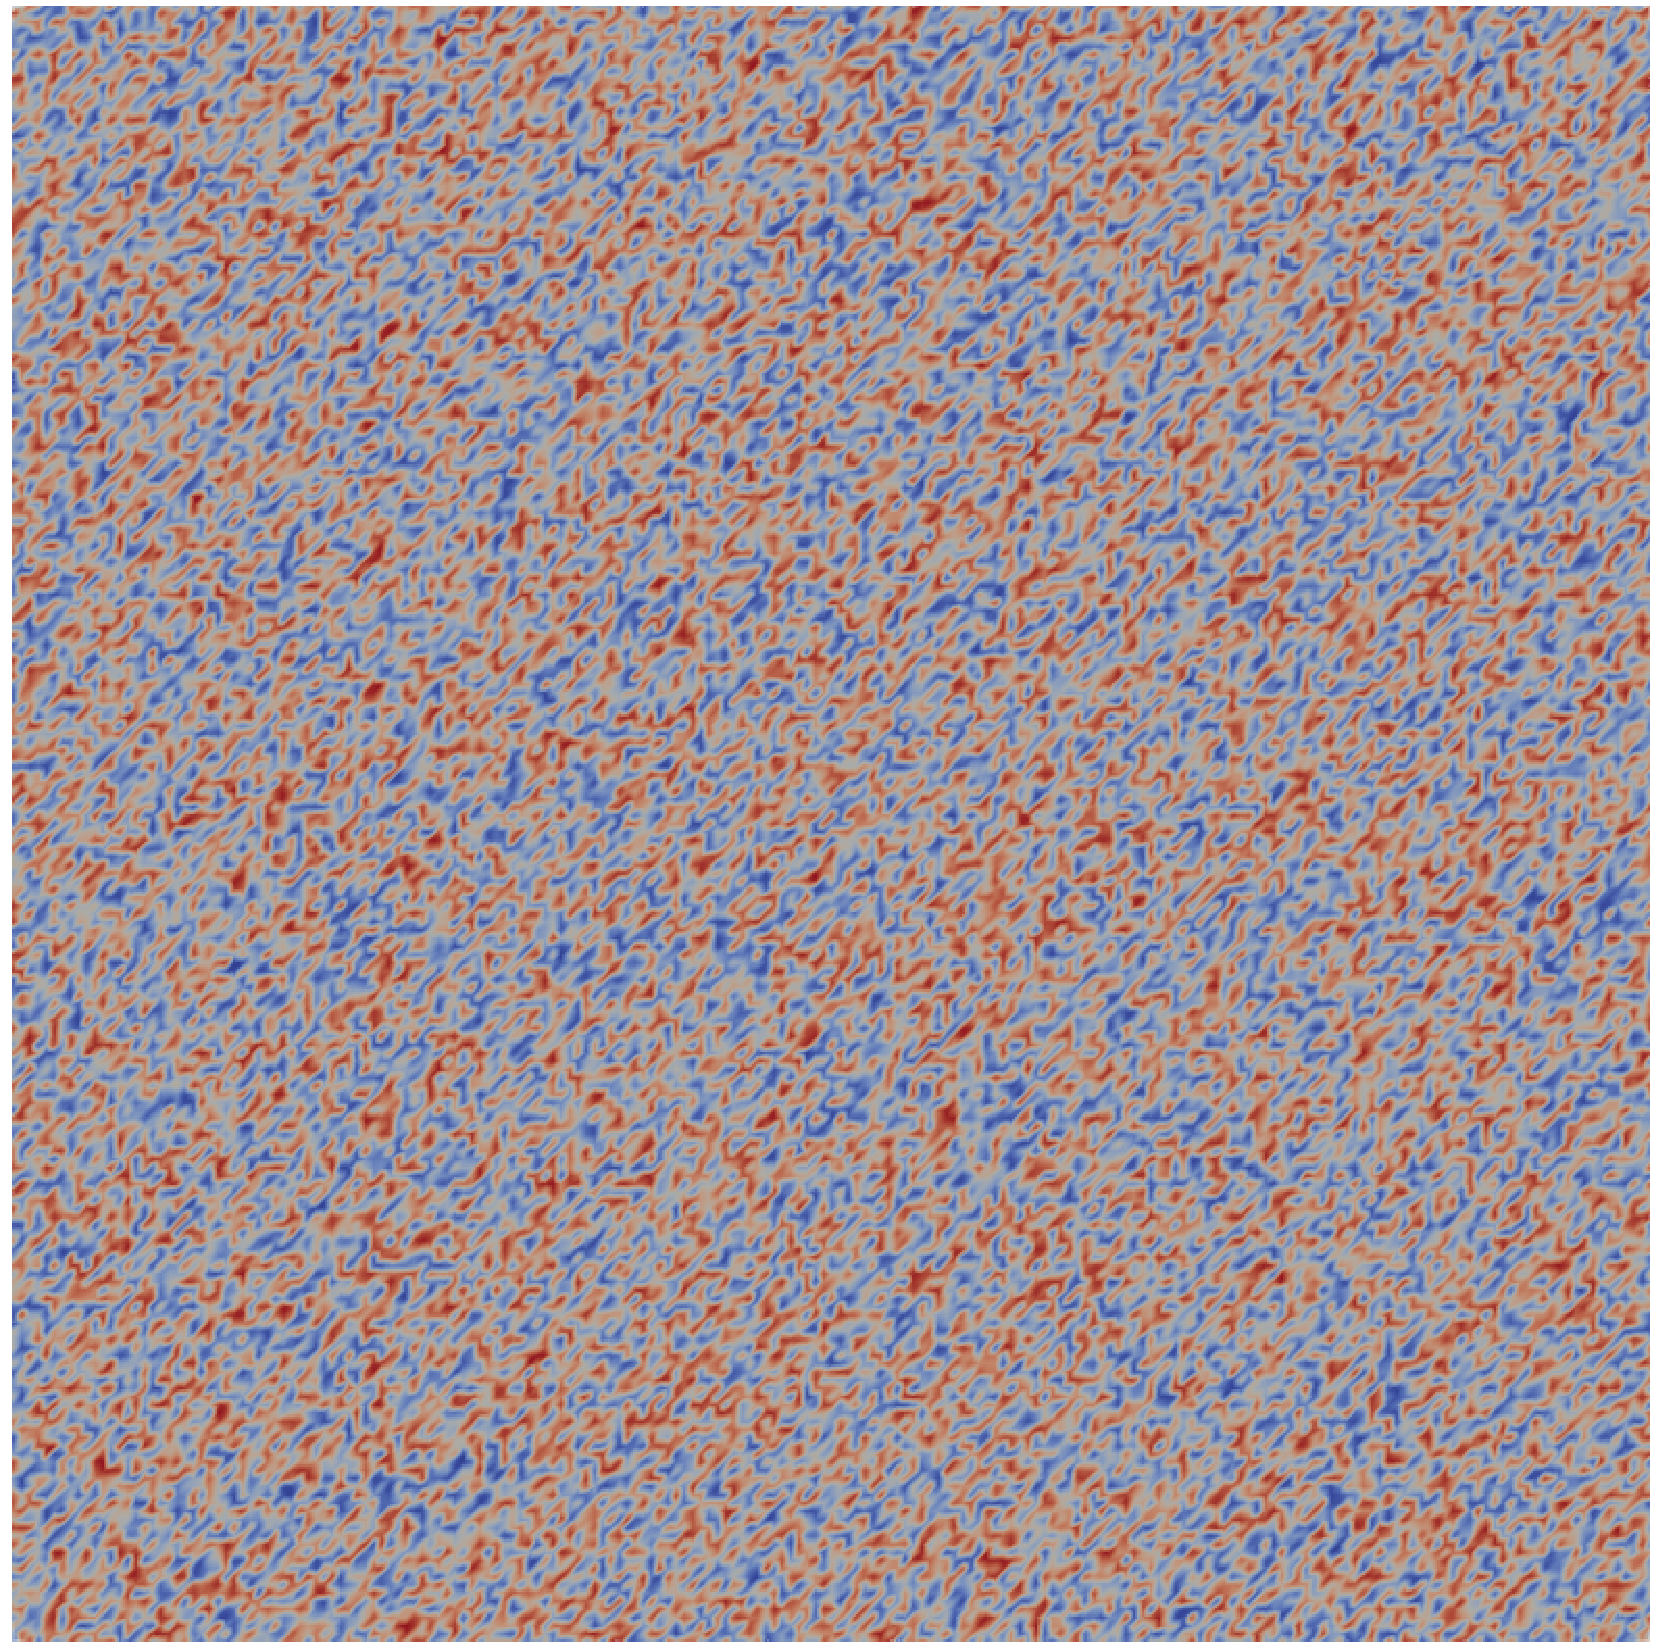
\includegraphics[width=0.95\textwidth]{Imagenes/Maxwell2D/Maxwell2D_sim/Imagenes/t_0}
        \caption{$t=0$}
    \end{subfigure}
    \begin{subfigure}[t]{0.45\textwidth}
        \centering
        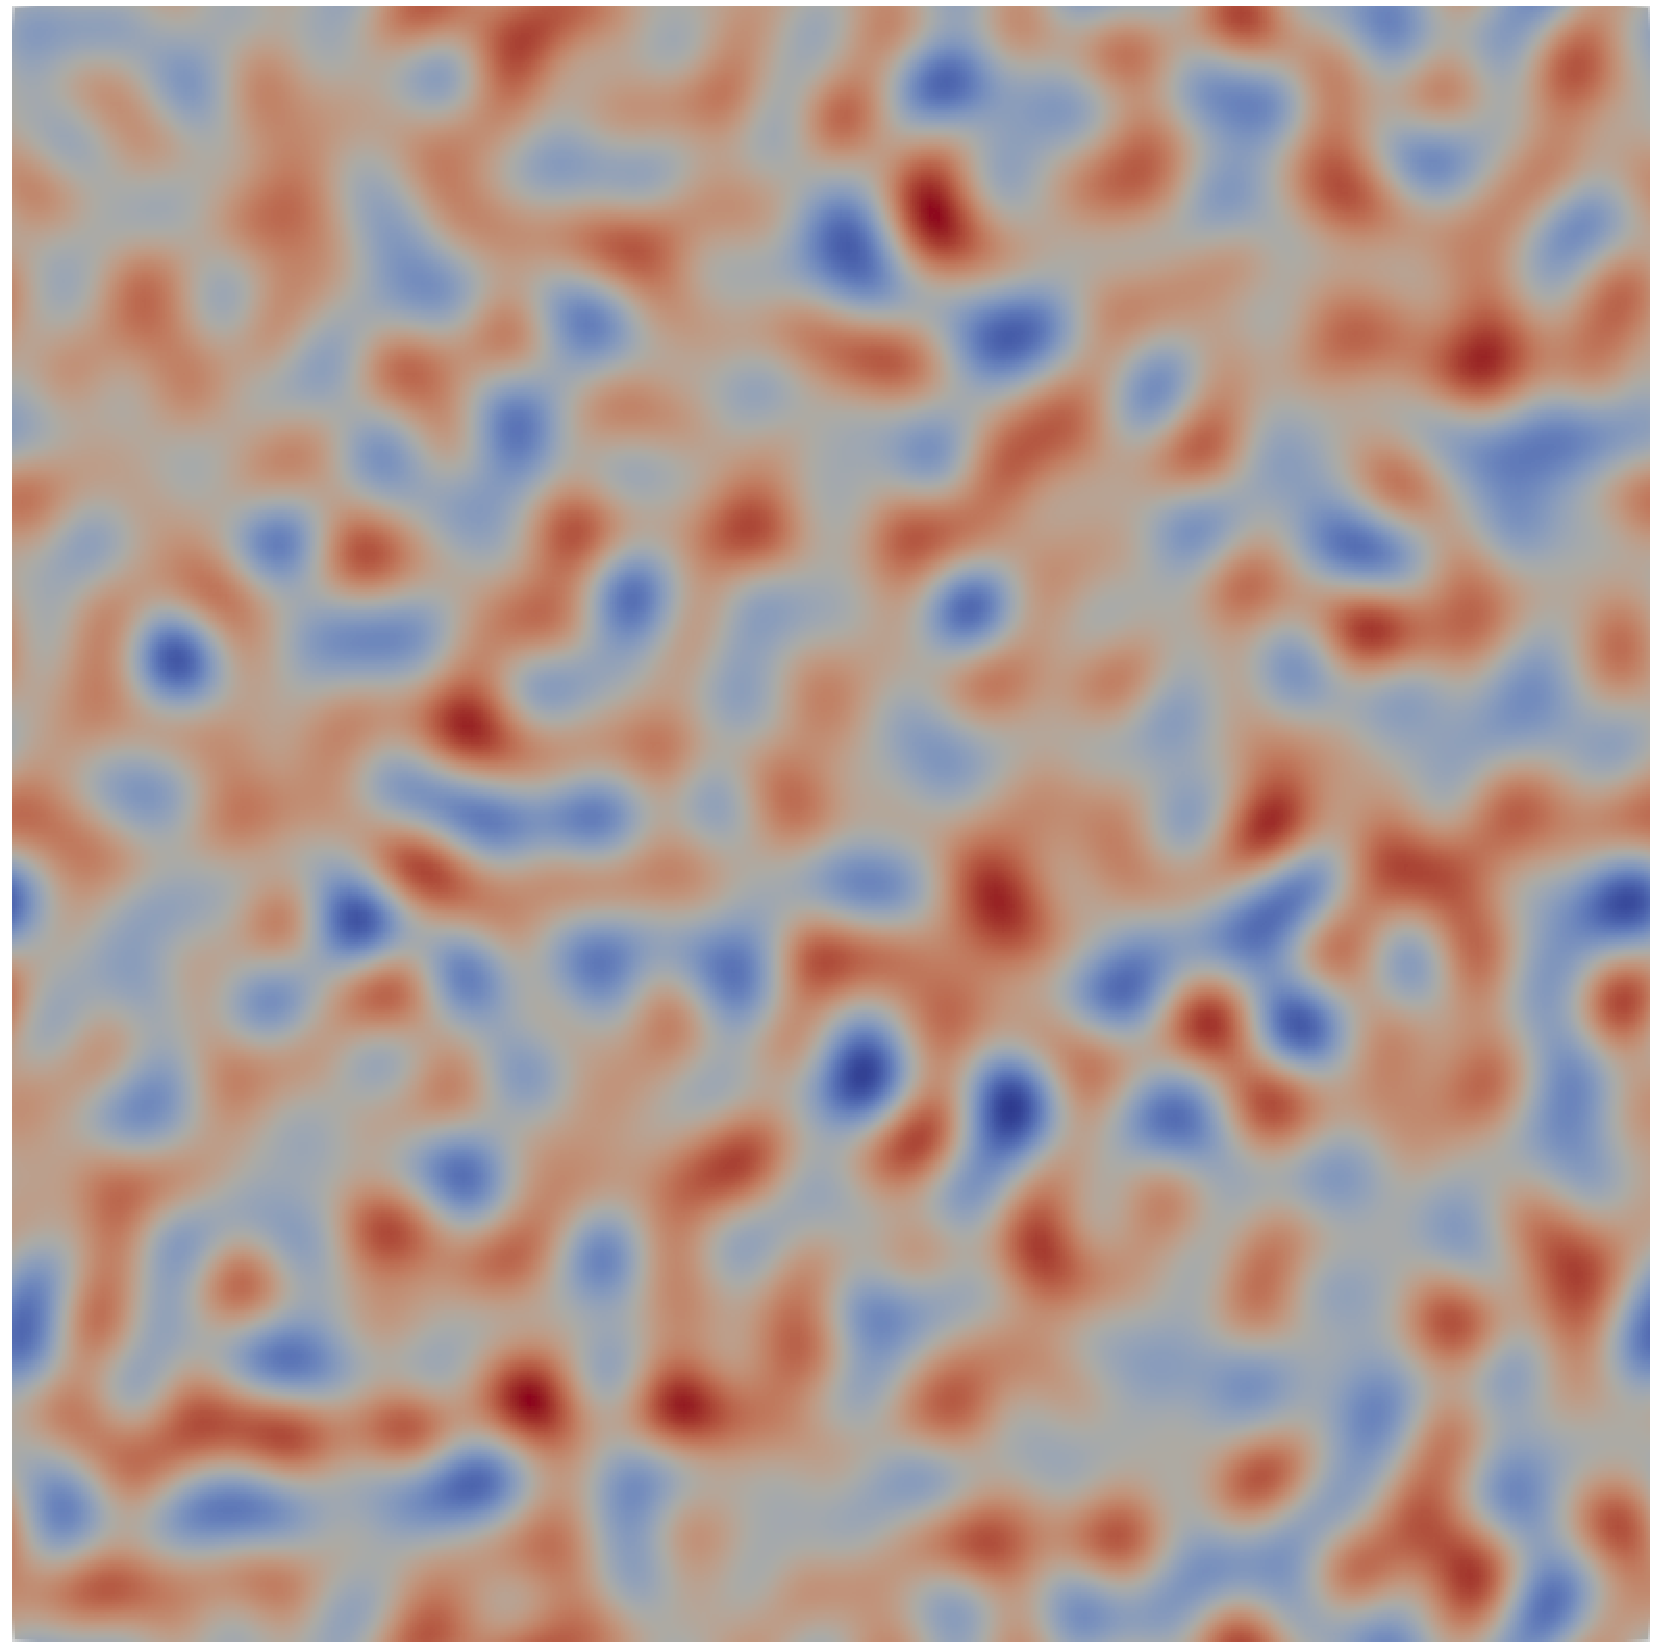
\includegraphics[width=0.95\textwidth]{Imagenes/Maxwell2D/Maxwell2D_sim/Imagenes/t_50}
        \caption{$t = 50$}
    \end{subfigure}
    \begin{subfigure}[t]{0.45\textwidth}
        \centering
        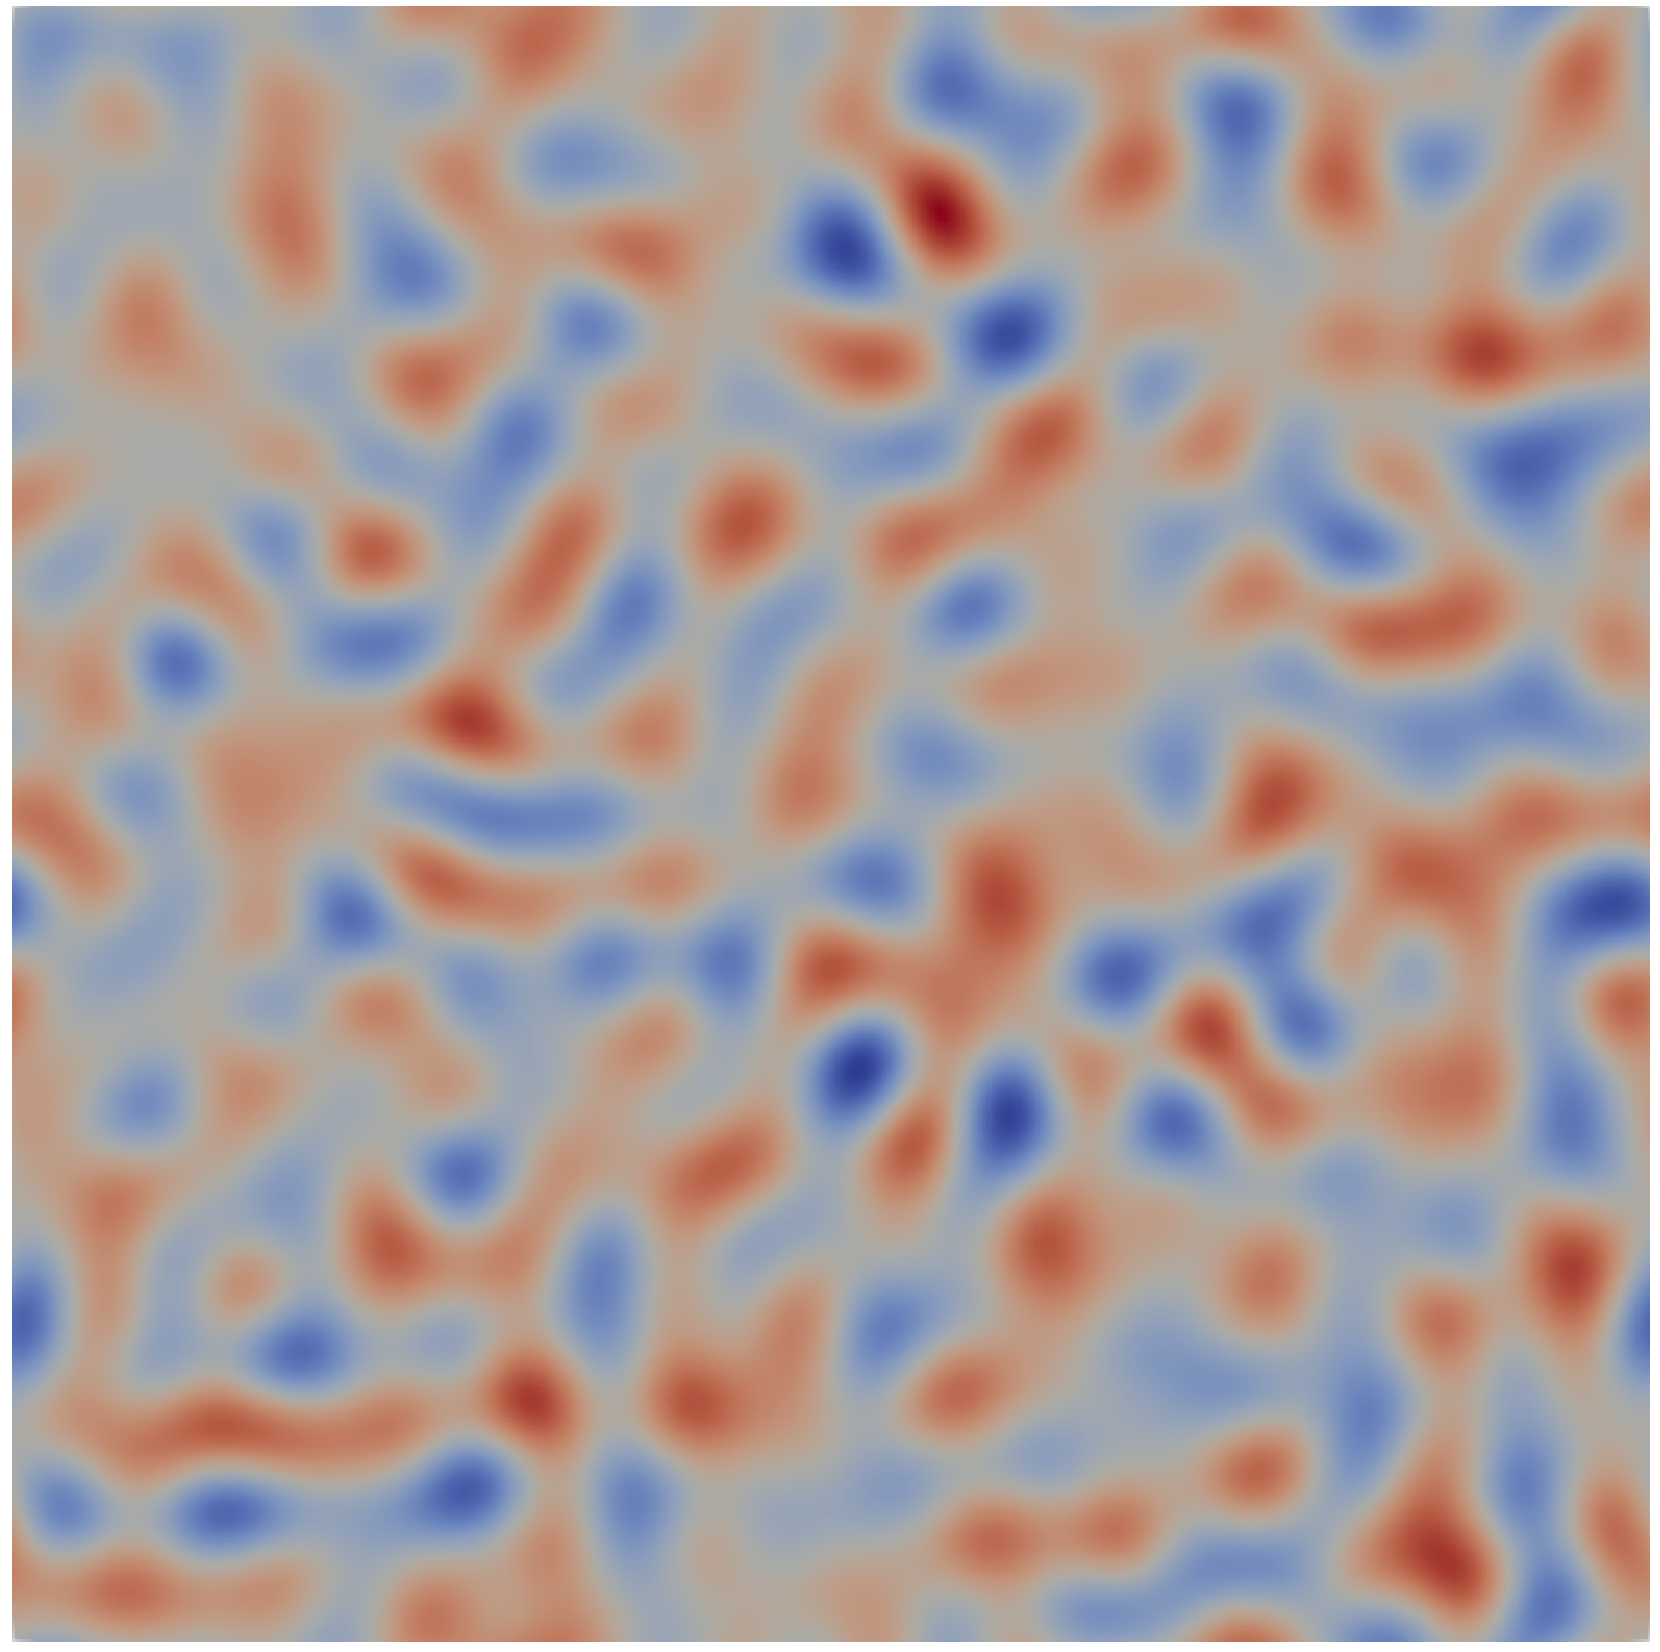
\includegraphics[width=0.95\textwidth]{Imagenes/Maxwell2D/Maxwell2D_sim/Imagenes/t_100}
        \caption{$t = 100$}
    \end{subfigure}    
    \begin{subfigure}[t]{0.45\textwidth}
        \centering
        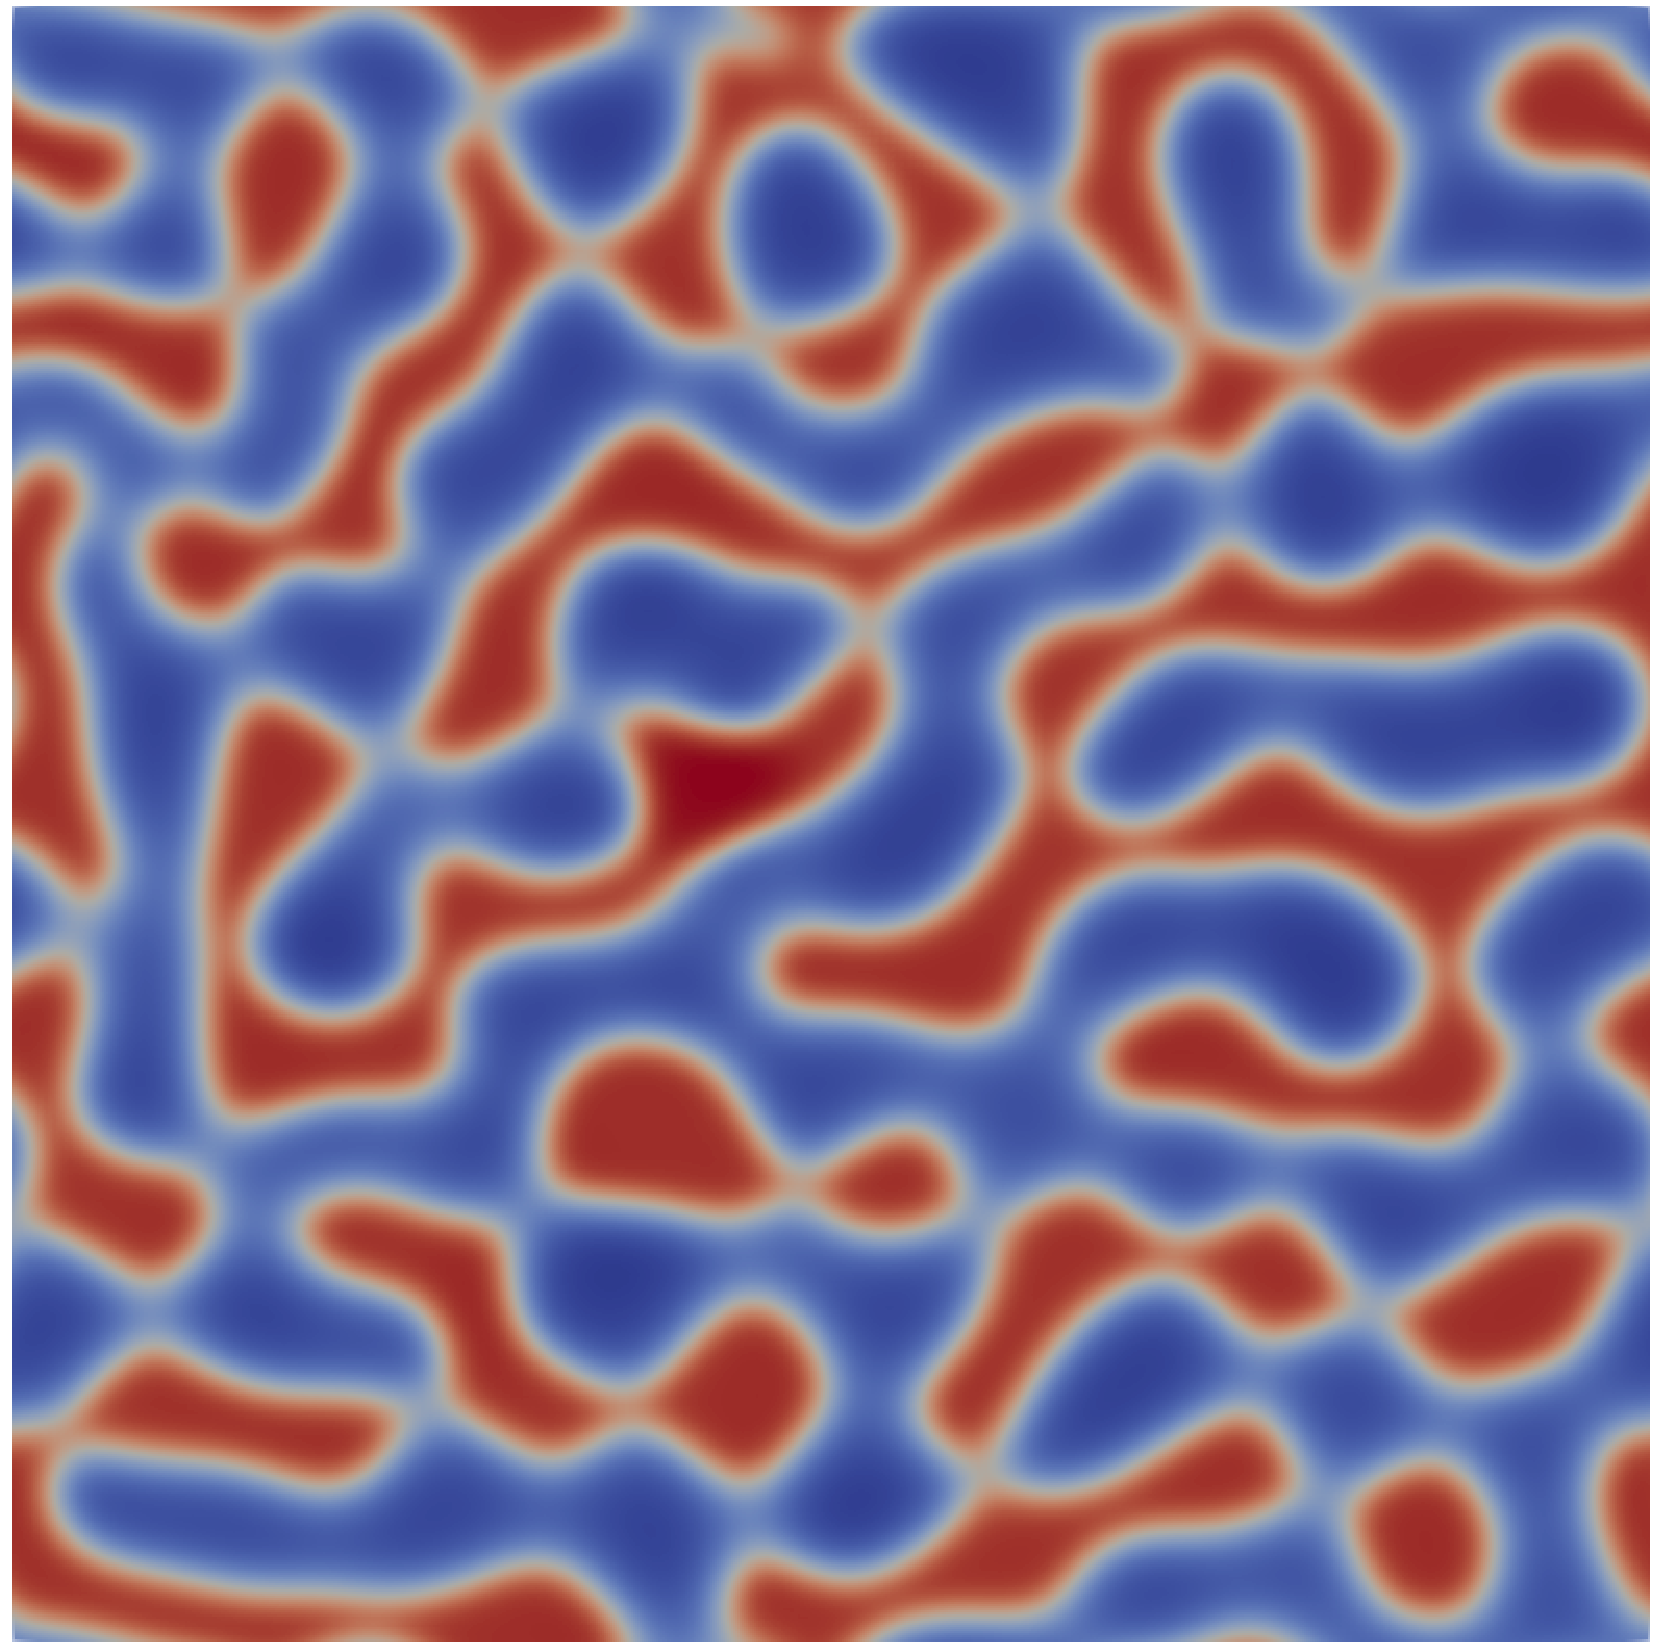
\includegraphics[width=0.95\textwidth]{Imagenes/Maxwell2D/Maxwell2D_sim/Imagenes/t_500}
        \caption{$t = 500$}
    \end{subfigure}    
    \begin{subfigure}[t]{0.45\textwidth}
        \centering
        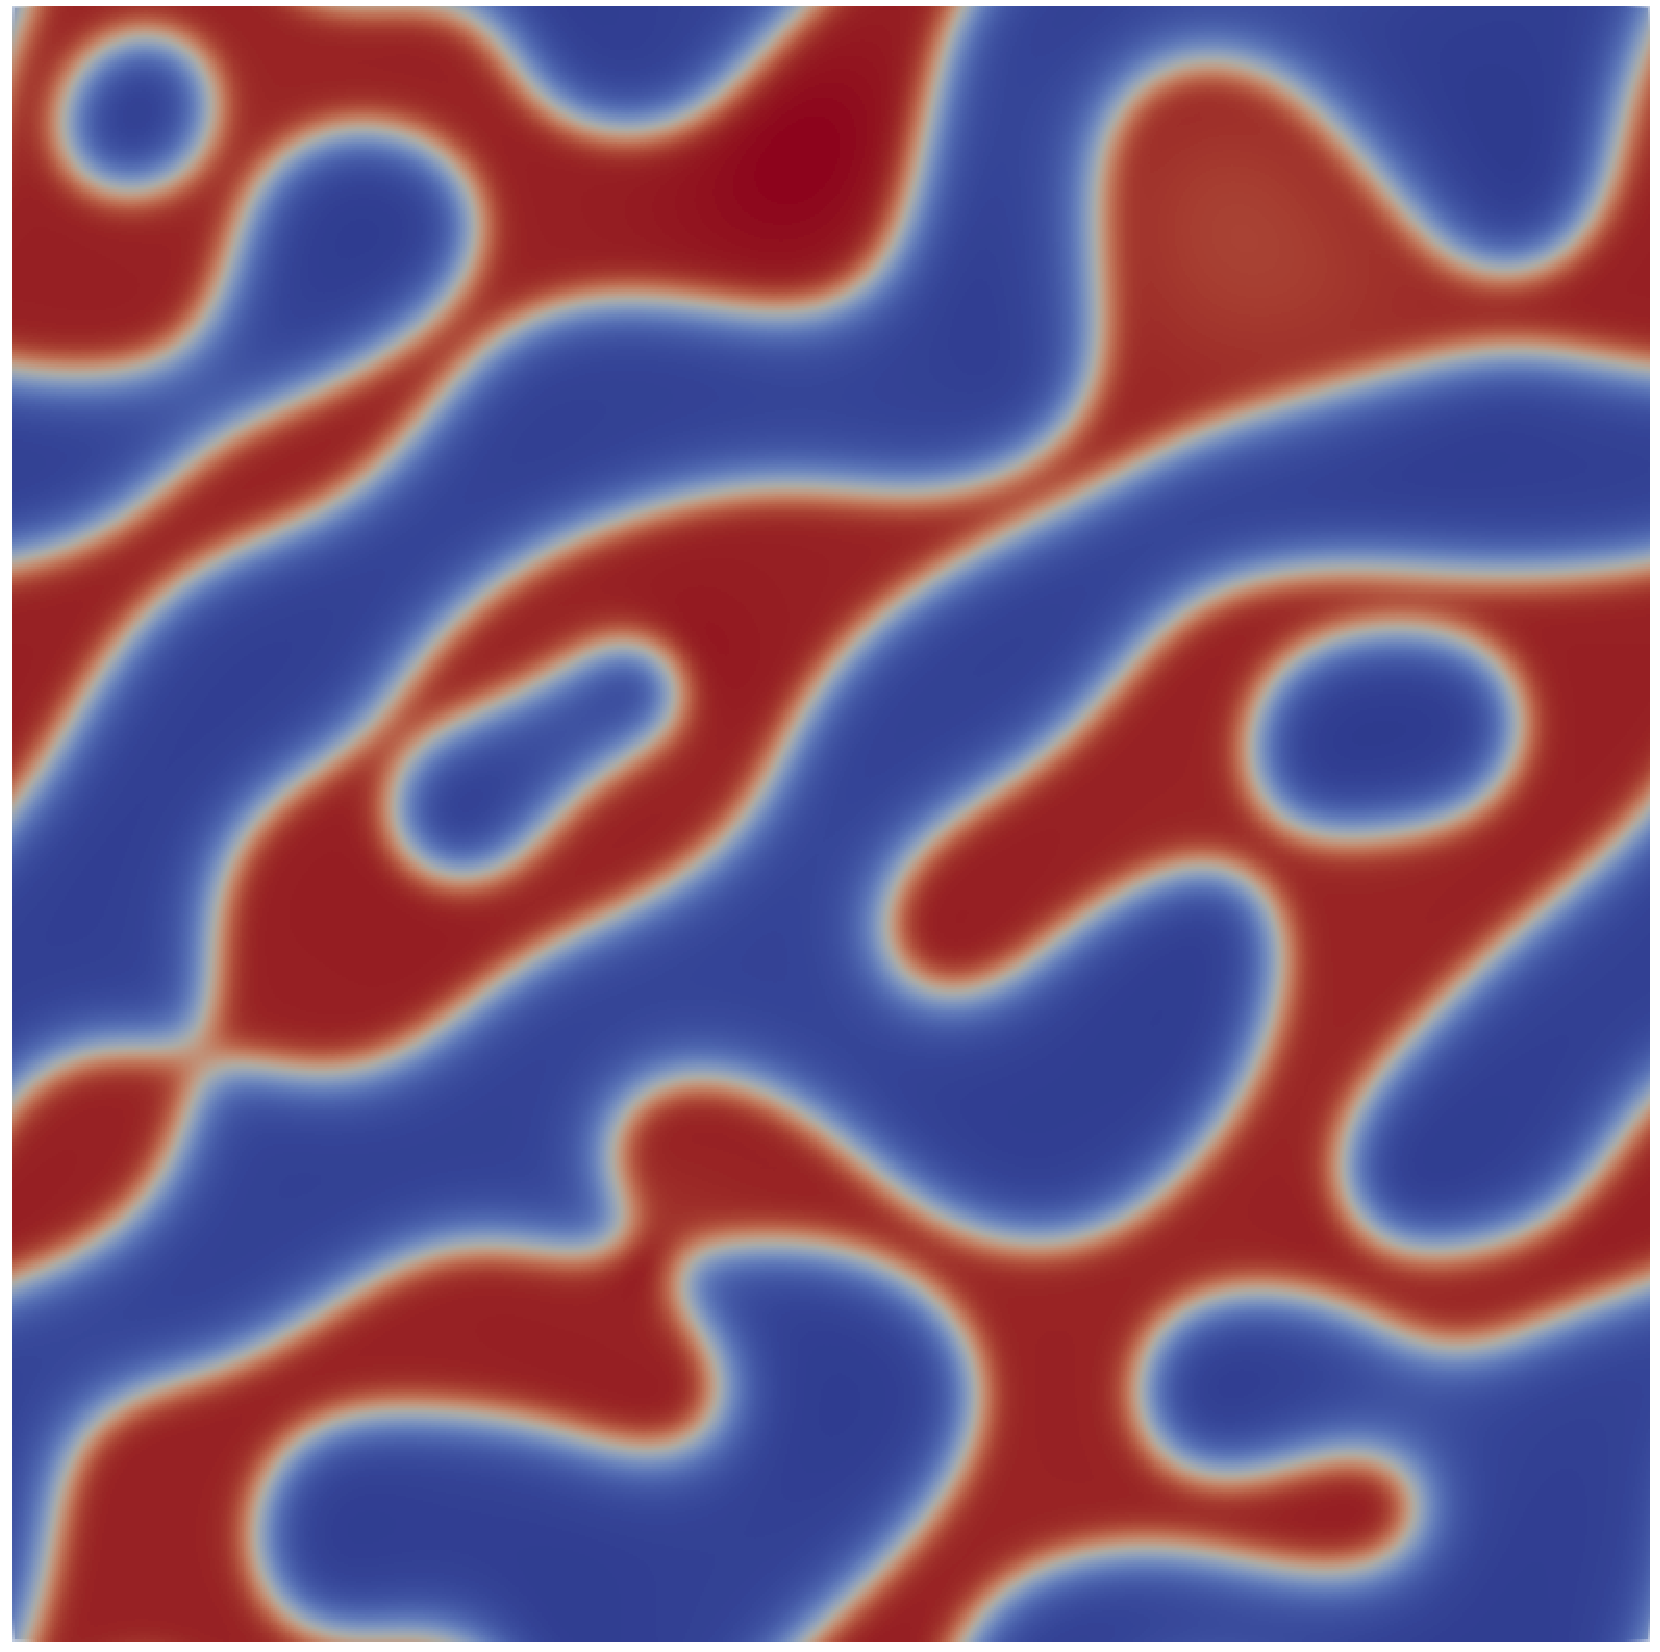
\includegraphics[width=0.95\textwidth]{Imagenes/Maxwell2D/Maxwell2D_sim/Imagenes/t_1000}
        \caption{$t = 1000$}
    \end{subfigure}
    \begin{subfigure}[t]{0.45\textwidth}
        \centering
        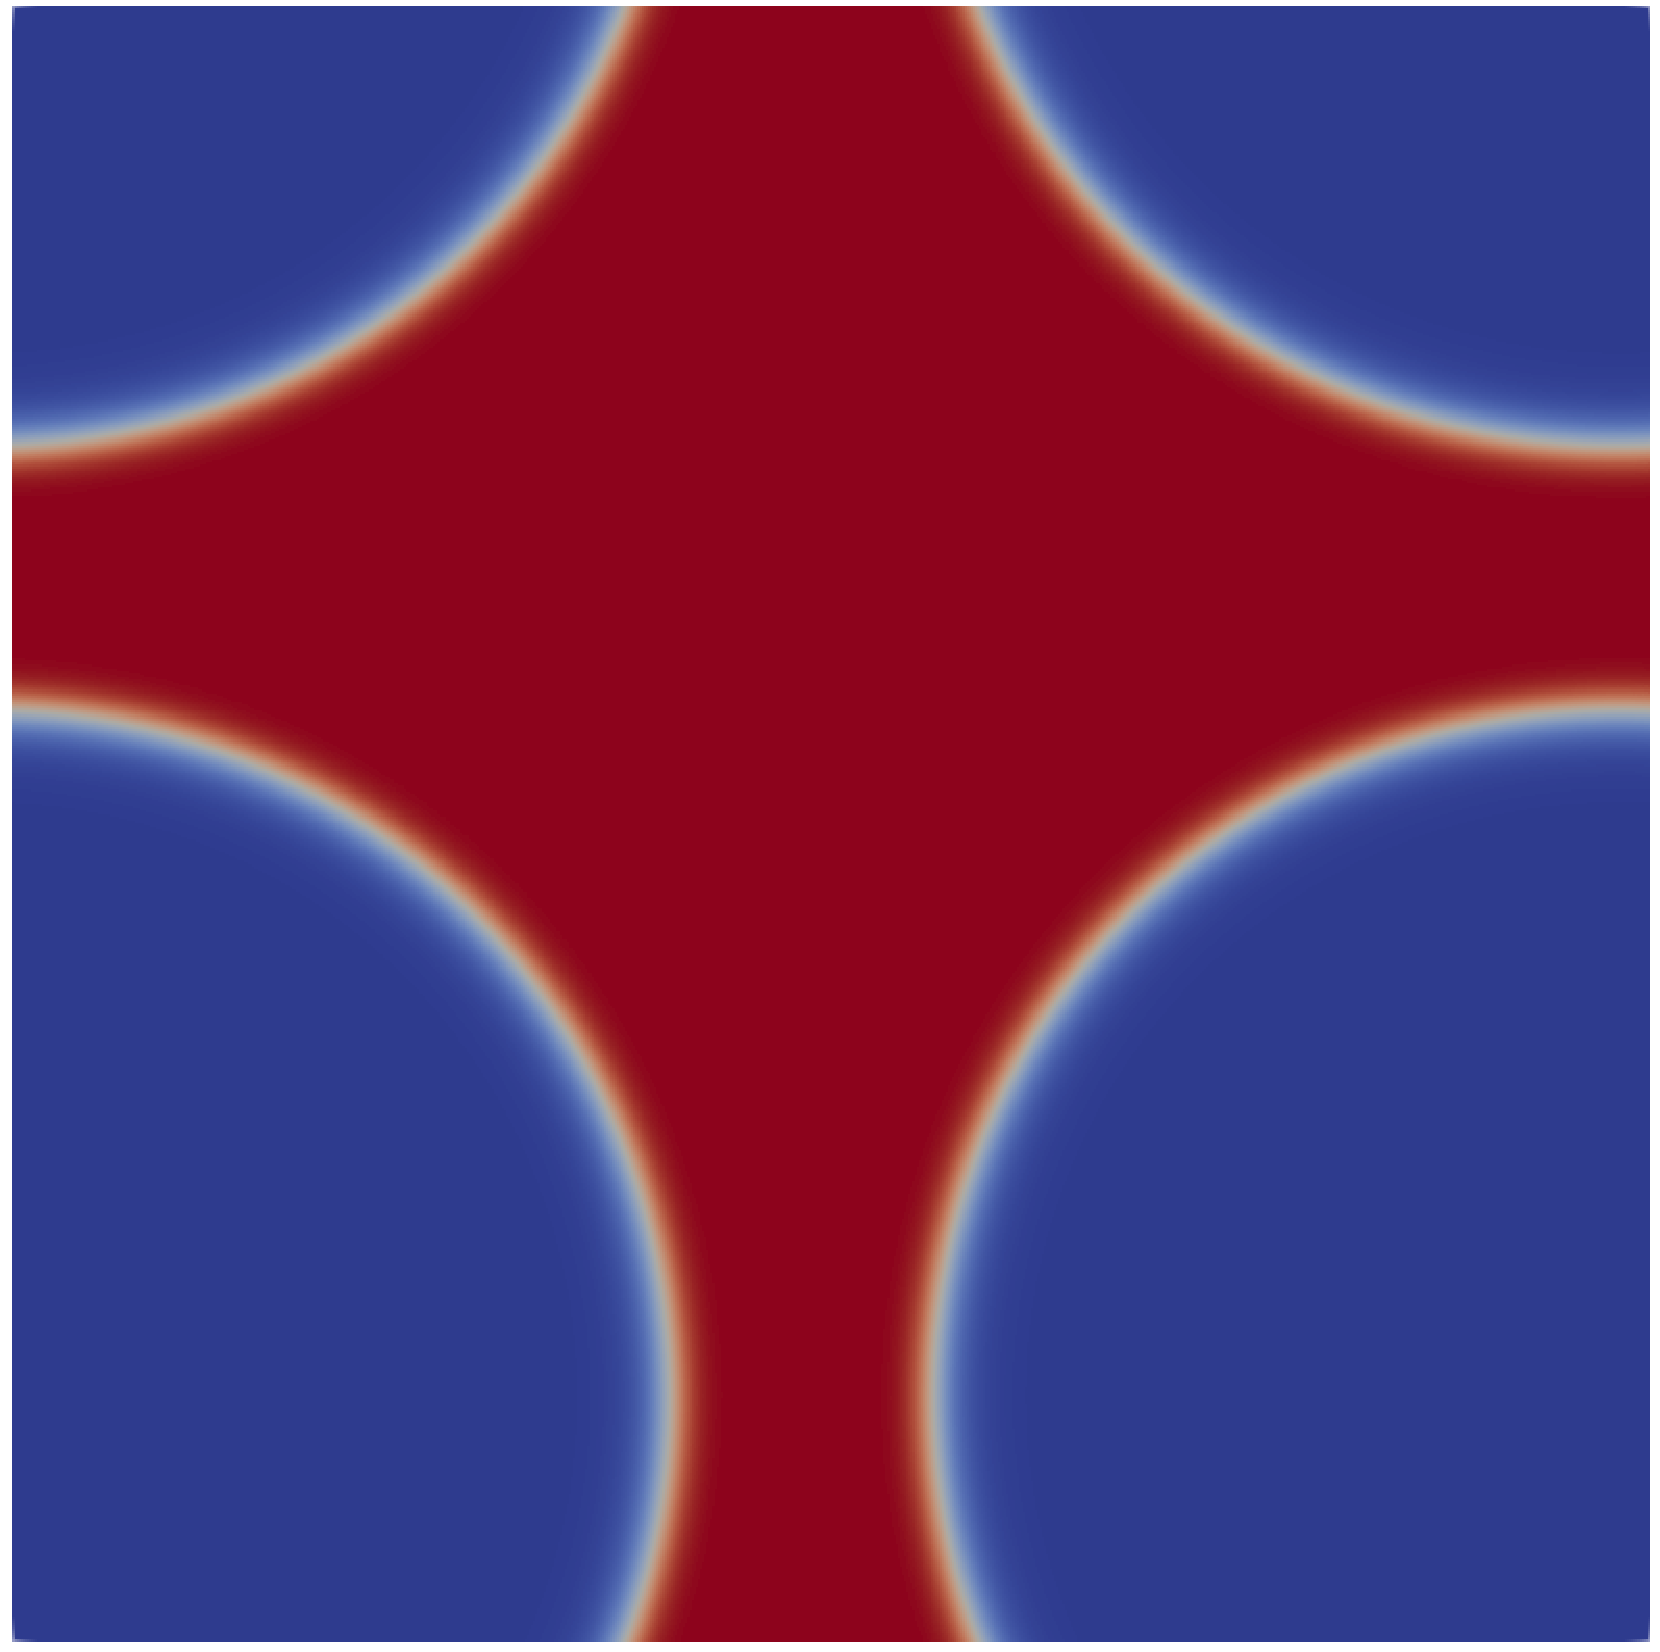
\includegraphics[width=0.95\textwidth]{Imagenes/Maxwell2D/Maxwell2D_sim/Imagenes/t_50000}
        \caption{$t = 50000$}
    \end{subfigure}        
    \caption{Evoluci\'on de una regi\'on tridimensional, peri\'odica, isot\'ermica y sin fuerzas externas, usada para verificar la regla de construcci\'on de Maxwell. La regi\'on mostrada corresponde a la fase de menor densidad.}
    \label{fig:maxwell_3d}
\end{figure}
\FloatBarrier

%
%\chapter{Simulaci\'on de ebullici\'on en FC72}



%% % Podemos usar cualquiera de los dos comandos: \input o \include para incluir el texto
%% \input{cap1}
%% \include{cap2}


%% \appendix
%% \include{apend1}

 \begin{biblio}
    \bibliographystyle{ibtesis}
 	\bibliography{Library}
 \end{biblio}


%% \begin{postliminary}

%% \begin{seccion}{Publicaciones asociadas}
%%   \begin{enumerate}
%%   \item Mi primer aviso en la revista \textbf{ABC}, 1996
%%   \item Mi segunda publicaci\'{o}n en la revista \textbf{ABC}, 1997
%%   \end{enumerate}
%% \end{seccion}

%% \begin{seccion}{Agradecimientos}
%% A todos los que se lo merecen, por merecerlo
%% \end{seccion}

%% \end{postliminary}

\end{document}

